% !TEX program = lualatex
\documentclass[11pt,a4paper]{article}
\title{\textbf{HEAT STRESS AND RUNNING PERFORMANCE}\\[0.4em]
\large Modeling equal-effort pace from race results}
\date{}
\usepackage[a4paper, top=2cm, bottom=2cm, left=1.7cm, right=1.7cm]{geometry}
\usepackage{fontspec}
\usepackage[english]{babel}
\usepackage{amsmath,amssymb}
\usepackage{amsthm}
\usepackage{unicode-math}
\usepackage[dvipsnames]{xcolor}
\usepackage{graphicx}
\graphicspath{ {./images/en/} }
\usepackage{array}
\usepackage{booktabs}
\usepackage{needspace}
\usepackage{parskip}
\usepackage[font=small, labelfont=bf]{caption}
\usepackage{fancyhdr}
\usepackage{etoolbox}
\usepackage[round, authoryear]{natbib}
\usepackage{hyperref}

\pagestyle{fancy}
\setlength{\headheight}{14pt}
\fancyfoot[R]{\small{G.LEPERE}}
\fancyfoot[L]{gabin.lepere.pro@gmail.com}
\fancyhead[L]{Heat stress and running performance}
\fancyhead[R]{2026}

\definecolor{accent}{HTML}{B4462E}   % terracotta
\definecolor{encre}{HTML}{23252B}
\definecolor{gris}{HTML}{8C857A}
\definecolor{darkgreen}{RGB}{0,100,0}

\IfFontExistsTF{EBGaramond-Regular.otf}
  {\setmainfont{EBGaramond}[Extension=.otf, UprightFont=*-Regular,
     ItalicFont=*-Italic, BoldFont=*-SemiBold, BoldItalicFont=*-SemiBoldItalic,
     Numbers=OldStyle]
   \newfontfamily\chiffres{EBGaramond}[Extension=.otf, UprightFont=*-SemiBold,
     Numbers=Lining]}
  {\setmainfont{EB Garamond}[Numbers=OldStyle, BoldFont={* SemiBold}]
   \newfontfamily\chiffres{EB Garamond SemiBold}[Numbers=Lining]}
\IfFontExistsTF{Garamond-Math.otf}
  {\setmathfont{Garamond-Math.otf}[StylisticSet={7,9}]}
  {\setmathfont{Latin Modern Math}}

\color{encre}
\setlength{\parindent}{0pt}
\setlength{\parskip}{0.3em}
\linespread{1.04}
\setlength{\emergencystretch}{1.5em}
\AtBeginEnvironment{tabular}{\addfontfeatures{Numbers={Lining,Monospaced}}}
\hypersetup{colorlinks=true, linkcolor=encre, citecolor=accent, urlcolor=accent,
  pdftitle={Heat stress and running performance}, pdfauthor={G. Lepere}}

\newcommand{\E}{\mathbb{E}}
\DeclareMathOperator{\Var}{Var}
\DeclareMathOperator{\Cov}{Cov}
\DeclareMathOperator{\Corr}{Corr}
\newcommand{\PB}{\mathrm{PB}}
\newcommand{\WBGT}{\mathrm{WBGT}}
\newcommand{\dd}{\mathrm{d}}
\newtheorem*{theorem}{Theorem}

\begin{document}
\maketitle
\vspace{-3em}
\begin{center}
\textbf{Written by G.LEPERE}
\end{center}
\vspace{1.5em}

{\itshape
How much does heat slow a runner down at equal effort? To answer this question without any physiological
measurement, we collected about 21,000 race performances, from the 800~m to the marathon, run between 2023 and 2026
in one hundred cities across 36~countries. Each performance is expressed relative to the personal best the athlete
held before the race, and each race is linked to the heat stress it was run in, measured by the WBGT reconstructed hour
by hour from meteorological reanalyses. Three difficulties shape the study: result lists are truncated by time, which
attenuates the apparent effect of heat; weather is not randomly distributed across events, countries and fields; and
runners in the same race are not independent observations, so that 10,398 performances are worth only about 1,900
independent observations. On cities never seen during training, we compare models of increasing complexity:
penalized regressions, mixed-effects models, gradient-boosted trees and neural networks. Their accuracies are
statistically indistinguishable; their degradation curves are not. We therefore retain an interpretable mixed model
in which the effect of heat depends on the event group: at a WBGT of 25~°C, the estimated slowdown is zero over middle
distances and reaches 3.1\% in the marathon (95\% interval: 2.3 to 4.1\%) relative to a WBGT of 15~°C. Once inverted,
this model provides an ``equal-effort'' pace conversion together with its uncertainty, and refuses to extrapolate
outside the observed domain.\par}

\vspace{0.8em}
\textbf{Keywords.} Thermoregulation, WBGT, truncation, mixed-effects models, grouped cross-validation, gradient
boosting, neural networks, conformal prediction.

\newpage
\tableofcontents
\newpage

\section{Introduction}

The summer of 2026 gave the link between weather and athletic performance a particular topicality. June 2026 was the
hottest June ever recorded in France ($+3.8$~°C above normal); July then broke the all-time monthly heat record since
measurements began, with a national average of 24.9~°C (Météo-France). These conditions did not prevent elite
athletes from performing, at the cost of adjustments. For the first time in its history, the Tour de France shortened
a stage because of the heat (Malemort--Ussel, July~12). At the Paris Diamond League meeting on June~28, only the
professional events were held, and they produced world-class times: 1:53.80 for Audrey Werro over 800~m, the third
best performance in history, and 3:28.00 for Cameron Myers over 1,500~m. Amateur athletes, by contrast, suffered a
great deal: without medical support or adjusted schedules, they had to keep up their training sessions through
several weeks of heatwave.

At the same time, heat training has become popular. The 2025 World Athletics Championships in Tokyo, in September,
were held in temperatures above 30~°C and humidity above 80\%. Federations prepared their athletes in climatic
chambers, at training camps in hot climates and with cooling protocols, and World Athletics launched a study on the
acclimatization of its marathon runners and race walkers. It builds on the 2019 Doha championships: 63\% of the
athletes surveyed there had followed a specific heat preparation, and those athletes had generally performed better.

Amateurs obviously have no access to climatic chambers or to the physiological monitoring of professionals. Yet the
benefits of acclimatization are well established. The expert consensus of \citet{racinais2015} identifies it as the
most effective intervention to reduce physiological strain and preserve performance in hot environments: repeated
exposures to exercise in the heat over one to two weeks. \citet{lorenzo2010} even observed, in trained cyclists, a
performance gain of about 7\% after ten days of acclimatization, including in cool conditions, and
\citet{ronnestad2022} showed that five weeks of training in a heat suit increase the hemoglobin mass of elite
cross-country skiers by about 30~g compared with a control group.

Beyond any deliberate preparation, one does not choose the weather. A runner regularly has to complete a planned
session in strong heat or high humidity, and the same pace no longer corresponds to the same effort. Running at the
planned pace then amounts to a harder session than intended, with a risk for the training plan, or even for health.
Sensations remain the safest guide: slowing down when the effort becomes too costly protects better than any target
pace. A more delicate question remains: \emph{how much do weather conditions actually slow a runner down at equal
effort?} Answering it would make it possible to adjust one's pace in advance rather than by feel, to interpret fairly
a time achieved in strong heat, or to compare two sessions run in different conditions.

Several studies have addressed this question. \citet{ely2007} analyzed seven major marathons: among the best men, the
gap to the course record rises from 1.7\% for a WBGT of 5 to 10~°C to 4.5\% between 20 and 25~°C, and slower runners
are affected even more. \citet{mantzios2022} extended the analysis to 1,258 endurance races (from the 3,000~m
steeplechase to the marathon, from 1936 to 2019, in 42~countries). They place the best performances between 7.5 and
15~°C of WBGT, with a decline of 0.3 to 0.4\% per degree beyond. The reference indicator in these studies is the WBGT
(\emph{Wet Bulb Globe Temperature}), which combines air temperature, humidity, wind and solar radiation into a single
measure of heat stress; the American College of Sports Medicine and World Athletics use it to set their risk
thresholds. These studies, however, describe winners' performances aggregated by race. They do not directly tell a
runner what pace to run today to produce the same effort as in ideal conditions.

This is the purpose of the present work. The question we ask is the following:
\begin{quote}
\itshape For a given temperature $T$ and relative humidity $RH$ (and, when known, wind, solar radiation and altitude),
at what actual speed $X$ should one run to produce the same effort as at speed $Y$ in reference conditions?
\end{quote}
Since effort is not measured, the approach is necessarily indirect. We first learn, from actual race performances,
\emph{how much conditions slow an athlete down relative to their own level}, and then \emph{invert} this model to
convert a reference speed into an equal-effort speed. To this end, we built a data set of about 21,000 performances,
from the 800~m to the marathon, achieved between 2023 and 2026 in 100 cities across 36~countries. Each performance is
expressed relative to the athlete's personal best before the race, and the weather is reconstructed at the time and
place of the race from hourly reanalyses (ERA5), from which we compute the WBGT averaged over the race duration with
the physical model of \citet{liljegren2008}.

The article follows the order in which the work was carried out. Section~\ref{sec:framework} recalls the
physiological basis of thermoregulation, defines the WBGT and formulates the problem: the choice of target, the
reference conditions, and two pitfalls identified from the outset, the truncation of result lists and confounding
factors. Data exploration (section~\ref{sec:data}) sharpens these pitfalls, measures them, and reveals a strong
dependence between runners of the same race; it dictates the validation protocol of section~\ref{sec:validation}.
Sections~\ref{sec:linear} to~\ref{sec:networks} build models of increasing complexity, from linear regressions to
neural networks, through mixed models and gradient boosting; section~\ref{sec:comparison} tunes them and compares
them on unseen cities. Section~\ref{sec:interpretation} interprets what these models have learned and derives the
model of the final tool, whose prediction uncertainty is quantified in section~\ref{sec:uncertainty} and whose use is
described in section~\ref{sec:tool}. Section~\ref{sec:discussion} discusses the limitations of the whole.

\section{Physiological background and problem formulation}\label{sec:framework}

\subsection{Thermoregulation during exercise}\label{sec:physio}

A runner's heat balance reads, in watts,
\[
S = M - W_{\text{mech}} \pm R \pm C - E,
\]
where $S$ is the heat \emph{stored} by the body, $M$ the \emph{metabolic} energy production of the muscles and
$W_{\text{mech}}$ the \emph{mechanical work} performed. Since muscular efficiency is only 20 to 25\%, about three
quarters of $M$ end up as heat. $R$ and $C$ are the exchanges by \emph{radiation} (sun, ground, surroundings) and by
\emph{convection} (contact with moving air); they can cool the runner as well as heat them, hence the $\pm$ sign. $E$
is the loss through \emph{evaporation} of sweat. If $S > 0$ persistently, core temperature rises.

The orders of magnitude are considerable. The energy cost of running is about
$4~\text{J}\,\text{kg}^{-1}\,\text{m}^{-1}$: at $5.5$~m/s, the pace of a 2:08 marathon, a 60~kg athlete expends
$4 \times 60 \times 5.5 \approx 1{,}300$~W. With an efficiency of 20 to 25\%, more than 1,000~W of heat must be
dissipated continuously, the equivalent of an electric heater. When air temperature approaches skin temperature (33
to 35~°C), the exchanges $C$ and $R$ become small, or even negative, and only evaporation remains. Evaporation depends
on the water vapor pressure difference between skin and air: it is hindered by humidity, and hot, saturated air is the
most unfavorable case. Solar radiation adds a load of several hundred W/m², whereas wind, on the contrary, increases
convective and evaporative exchanges.

If heat is not dissipated, core temperature rises. Skin blood flow, needed to carry heat to the skin, then competes
with muscle blood flow: the heart cannot supply both at their maximum. The effective maximal oxygen uptake
$\dot V\mathrm{O}_2\max$ decreases and the athlete slows down, often in anticipation: they regulate their pace so as
not to reach a critical temperature, before even getting there. The effect grows with the duration of the effort,
since the stored heat $S$ accumulates over time. It is small over 800~m (about two minutes), where core temperature
does not have time to rise and where warm, less dense air may even help by reducing aerodynamic drag; it becomes
large in the marathon, which lasts two to three hours. In international championships, \citet{mantzios2022} find an
optimum WBGT between 7.5 and 15~°C and a degradation of 0.3 to 0.4\% per degree beyond; \citet{ely2007} observe in
the marathon a progressive slowdown from 5 to 25~°C of WBGT, more pronounced among slower runners.

Altitude acts through another mechanism. Atmospheric pressure, and with it the partial pressure of oxygen, decreases
by about 11\% per 1,000~m. The blood carries less oxygen, and $\dot V\mathrm{O}_2\max$ drops by about 6 to 8\% per
1,000~m above 500 to 1,000~m. Endurance events, limited by oxygen supply, suffer from it, whereas short events benefit
from the lower air density. Our data include races in Mexico City (about 2,200~m), Bogotá (2,600~m), Kigali, Boulder,
Guadalajara or Lanzhou (about 1,500~m).

\subsection{Measuring heat stress: the WBGT}\label{sec:wbgt}

The WBGT combines into a single index, expressed in degrees Celsius, the four factors of the heat balance, namely
temperature, humidity, wind and radiation:
\begin{equation}\label{eq:wbgt}
\WBGT = 0.7\,T_{nwb} + 0.2\,T_{g} + 0.1\,T_{a}.
\end{equation}
$T_{nwb}$ is the temperature of a \emph{natural wet-bulb} thermometer: surrounded by a wet wick, not artificially
ventilated and exposed to the sun, it is cooled by the evaporation of water, all the more so as the air is dry and
windy. It thus measures the capacity of the environment to remove heat by evaporation, as sweat does; in saturated
air, evaporation stops and $T_{nwb}$ joins $T_a$. $T_{g}$ is the temperature of a hollow \emph{black globe}, which
absorbs radiation from the sun and the ground and is cooled by the wind: it measures the radiative load. $T_{a}$,
finally, is the air temperature in the shade. The weights reflect the dominant role of evaporation in
thermoregulation during exercise: with 70\% of the weight on $T_{nwb}$, humidity strongly increases the WBGT at equal
temperature, and the WBGT is not a mere temperature.

The American College of Sports Medicine \citep{armstrong2007} associates risk flags with the WBGT for races: white
below 10~°C (risk of hypothermia), green from 10 to 18~°C, yellow from 18 to 23~°C, red from 23 to 28~°C and black
above 28~°C, a threshold at which cancelling the event is recommended.

The three temperatures in \eqref{eq:wbgt} are not measured on the courses. We \emph{computed} them with the physical
model of \citet{liljegren2008}, the reference method for estimating the WBGT from standard meteorological
measurements. This model writes the energy balance of the wet wick and that of the globe (direct and diffuse solar
radiation, thermal radiation, convection, evaporation) and solves them numerically from temperature, humidity, wind
speed, global solar radiation, pressure and the position of the sun, itself derived from the date, the time and the
coordinates of the site. Our implementation reproduces the Argonne reference code to within 0.01~°C. The WBGT was
computed \emph{every five minutes, from the start to the finish of each athlete}, then averaged: a 2:50 marathon
runner thus experiences the rise in temperature at the end of the morning, unlike a 2:05 winner. We will see that
this drift reaches a median of 3.7~°C in the marathon.

\subsection{What do we predict? The target}\label{sec:target}

Our approach is purely data-driven: no physiological measurement (heart rate, blood lactate, perceived exertion) is
available. We therefore approximate effort by \emph{race performance}, assuming that an athlete in a race produces a
maximal effort: if they run slower than usual in strong heat, it is because heat costs them speed at equal effort.
This assumption has its limits, since some athletes choose to ``manage'' their race in strong heat; we return to it in
section~\ref{sec:discussion}. To neutralize the level, sex and event of each athlete, each performance must be
compared with a \emph{reference specific to the athlete}. For performance $i$, with time $t_i$, by an athlete whose
personal best \emph{before the race} is $t_i^{\PB}$, the target is
\begin{equation}\label{eq:target}
y_i = 100\,\ln\frac{t_i}{t_i^{\PB}} .
\end{equation}

The logarithm has four virtues. The first is a reading as a percentage: for small $x$, $\ln(1 + x) \approx x$, so if
$t = 1.02\,t^{\PB}$, then $y = 100 \ln 1.02 \approx 1.98$; $y$ is expressed in ``logarithmic percent'', and $y = 2$
means about 2\% slower than one's personal best. The second is symmetry: $\ln(t/t^\star) = -\ln(t^\star/t)$, so that
running 2~points above or below one's best is treated in the same way, which is not the case for the ratio
$t/t^\star - 1$. The third is the equivalence between time and speed: over a fixed distance $d$, $v = d/t$, hence
$\ln(t/t^\star) = \ln(v^\star/v)$, and $y$ is also a relative speed gap, which will allow the result to be converted
directly into a pace. The last is additivity: multiplicative effects on time become additive on $y$. If heat
multiplies the time by $e^{\delta_1/100}$ and altitude by $e^{\delta_2/100}$, $y$ increases by $\delta_1 + \delta_2$;
this is the form suited to linear models. A value $y < 0$ corresponds to a new personal best.

Choosing the pre-race personal best as the reference is not innocuous. This best is published before the race and was
set elsewhere, in other conditions: it measures the athlete's level independently of the day's weather. A reference
that included the race itself would create an artifact. With the season's best, race included, a race run in
excellent conditions would become its own reference, and we would have $y \geq 0$ by construction. The pre-race
personal best is moreover available for 71\% of performances, against 36\% for the pre-race season's best, which we
use only as an indicator of \emph{form}.

\subsection{Two pitfalls: truncation and confounding}\label{sec:pitfalls}

As soon as the data were assembled, two difficulties appeared, which threaten any naive estimate of the effect of
heat.

\paragraph{The truncation of result lists.} Result lists are truncated by time. Major marathons only publish men
under 2:37 and women under 3:05, and small races only their first finishers. Let $T^{\max}_c$ denote the time of the
last runner listed in race $c$. An athlete appears in the data only if $t_i \le T^{\max}_c$, that is, if
\[
y_i \leq m_i = 100 \ln \frac{T_c^{\max}}{t_i^{\PB}} ,
\]
where $m_i$ is the \emph{truncation margin} of performance $i$: the largest slowdown that remains observable. In strong
heat, an athlete whose best is close to the threshold and who slows down disappears from the data; we only see those
who ran well relative to their level. The observed mean of $y$ is then pulled down, and the effect of heat is
underestimated. Section~\ref{sec:truncation} gives a formal proof, an empirical measurement and the remedy we
adopted.

\paragraph{Confounding factors.} A confounding factor is a variable $Z$ that influences both the exposure under study,
here the WBGT denoted $W$, and performance $y$. If it is omitted, its effect is wrongly attributed to the WBGT. Suppose
the true model is $y = \beta_0 + \beta_W W + \beta_Z Z + \varepsilon$, with $\varepsilon$ uncorrelated with $W$ and
$Z$, and that $y$ is regressed on $W$ alone. The estimated slope tends to
\begin{equation}\label{eq:omitted_bias}
\frac{\Cov(W, y)}{\Var(W)} = \frac{\beta_W\,\Var(W) + \beta_Z\,\Cov(W, Z)}{\Var(W)}
= \beta_W + \beta_Z\,\frac{\Cov(W, Z)}{\Var(W)} .
\end{equation}
This is the \emph{omitted-variable bias}. Its sign is that of the product $\beta_Z\,\Cov(W, Z)$: to predict in which
direction a factor biases the effect of heat, one must know both its effect on $y$ and its link with the WBGT. From the
outset, we excluded championship races, too prone to tactical racing. Among the unavoidable confounding factors, we pay
particular attention to the athlete's profile (level, age, sex), to the event, to the course and to the time of the
race.

\subsection{From model to pace: using the model both ways}\label{sec:both_ways}

Suppose we have a model $f$ that predicts $y$ from the conditions $\mathcal{C}$ and the characteristics $x$ of the
athlete and of the race. The degradation due to conditions $\mathcal{C}$, relative to reference conditions
$\mathcal{C}_{\text{ref}}$, is
\begin{equation}\label{eq:degradation}
\Delta(\mathcal{C}) = f(\mathcal{C}, x) - f(\mathcal{C}_{\text{ref}}, x),
\end{equation}
expressed in points of $y$. Consider an athlete who runs at speed $Y$ (time $t_Y$) in reference conditions and at
speed $X$ (time $t_X$) in conditions $\mathcal{C}$, for the same effort. The difference in target between the two
situations is
\[
\Delta = 100\ln\frac{t_X}{t^{\PB}} - 100\ln\frac{t_Y}{t^{\PB}} = 100\ln\frac{t_X}{t_Y} = 100\ln\frac{Y}{X},
\]
and the personal best cancels out. The equal-effort speed is therefore
\begin{equation}\label{eq:conversion}
X = Y\,\exp\!\left(-\frac{\Delta(\mathcal{C})}{100}\right),
\qquad\text{that is, } X \approx Y\,\Big(1 - \frac{\Delta}{100}\Big) \text{ to first order.}
\end{equation}
The degradation $\Delta$ depends on the athlete's level and race duration, hence on $Y$ itself. The inverse operation,
``I ran at speed $X$ at 30~°C, what is it worth in reference conditions?'', therefore requires solving the equation
$Y\,e^{-\Delta(\mathcal{C};\,Y)/100} = X$ numerically (section~\ref{sec:tool}).

It remains to set the reference conditions. We choose a reference WBGT $W_{\text{ref}} = 15$~°C, the upper end of the
``neutral'' range of 10 to 15~°C in the literature. A cooler reference would fall outside the domain of the track
data, which never go below 13.5~°C: the model could not be evaluated there without extrapolating. The reference wind
is a light breeze (2~m/s at a height of 10~m), the reference altitude is below 500~m, and the reference has no rain.

\section{The data and what they impose}\label{sec:data}

Exploratory analysis was not an end in itself. It served to identify what would condition the modeling: the ranges
of conditions covered and the missing combinations, the confounding factors, and the dependence structure between
observations. It turned the two pitfalls anticipated above into measured difficulties, and brought a third one to
light.

\subsection{Building the data set}\label{sec:dataset}

The data set was built in five steps. We first gathered the results of international track and road competitions
from 2023 to 2026, with one row per performance: sex, year of birth, event, meeting, city, date, local time, time, as
well as the season's best and personal best published before the race. The cities were then geocoded (coordinates,
time zone, altitude). Hourly weather was retrieved, through the Open-Meteo service \citep{zippenfenig2023}, from the
ERA5 \citep{hersbach2020} and ERA5-Land reanalyses and from the IFS model, then interpolated at five-minute steps. A
\emph{reanalysis} reconstructs past weather on a regular grid, with cells of about 9 to 30~km, by assimilating the
available observations into a numerical weather prediction model: it is an estimate of local weather, not a
measurement on the course. The Liljegren WBGT was then computed every five minutes and averaged over each athlete's
race (section~\ref{sec:wbgt}). The last step was to compute the target and the context variables, then to apply the
exclusions.

The fifteen events present were grouped into five \emph{event groups}, according to the surface (track or road) and
the duration of the effort, which conditions the expected effect of heat (table~\ref{tab:groups}). The structure of
the data is described by four nested grouping levels. A \emph{race} is defined by the meeting, the city, the date, the
event and the sex; a \emph{meeting} is a gathering (meeting, city and date) comprising several races; a \emph{course}
combines a city and an event, all editions together; a \emph{venue} is a city. A race thus belongs to a meeting and to
a course, which themselves belong to a venue.

Six context variables describe each performance. Age is the season year minus the year of birth. The \emph{level} is
$100\ln(t^{\PB}/t^{\PB}_{\text{med}})$, where $t^{\PB}_{\text{med}}$ is the median personal best for the sex and
event: it is negative for an athlete faster than the median. The \emph{form} is $100\ln(\text{SB}/t^{\PB}) \geq 0$,
where SB is the pre-race season's best; it is missing when there is no SB. The expected race duration is $t^{\PB}/60$,
in minutes. The local start time is, on the track, that of the start of the meeting. Finally, the truncation margin
$m_i$ was defined in section~\ref{sec:pitfalls}.

Of the 21,126 rows collected, 6,222 have no pre-race personal best, hence no reference, and 81 have an aberrant target,
outside the interval $[-15, 30]$: they are excluded. This leaves 14,823 valid performances, all associated with
weather data. The \emph{analysis sample} keeps only those whose truncation margin is at least 5\%, for reasons set out
in section~\ref{sec:truncation}. It contains 10,398 performances, spread over 396 races, 135 meetings, 172 courses and
100 venues in 36~countries.

\begin{table}[htbp]
\centering
\small
\caption{Composition of the analysis sample by event group. $\bar y$ is the mean of the target \eqref{eq:target}, in
percentage points.}
\label{tab:groups}
\begin{tabular}{@{}l>{\raggedright\arraybackslash}p{4.4cm}lrrrrr@{}}
\toprule
Group & Events & Typical duration & Perf. & Races & Venues & $\bar y$ & Women / men \\
\midrule
track middle distance & 800~m, 1,000~m, 1,500~m, mile & 2 to 4 min & 2,498 & 95 & 21 & 1.19 & 981 / 1,517 \\
track long distance & 2,000~m and 3,000~m steeplechase, 3,000~m, 5,000~m, 10,000~m & 5 to 35 min & 1,019 & 64 & 14 &
0.90 & 315 / 704 \\
short road races & road mile, 5~km and 10~km & 4 to 35 min & 1,890 & 87 & 30 & 1.44 & 438 / 1,452 \\
half marathon & half marathon & 1 h to 1 h 30 & 1,134 & 56 & 28 & 1.58 & 392 / 742 \\
marathon & marathon & 2 to 3 h & 3,857 & 94 & 41 & 2.18 & 1,575 / 2,282 \\
\bottomrule
\end{tabular}
\end{table}

The marathon is the most represented group (37\% of performances), track long distance the least (10\%). Men account
for 64\% of performances, with a marked imbalance in short road races, where there are three men for every woman.
$\bar y$ is positive in all groups and increases from track long distance (0.90\%) to the marathon (2.18\%). Track
events are concentrated in few venues (21 and 14): their weather conditions rest on few distinct situations.

\subsection{Distribution of the target and conditions covered}\label{sec:distributions}

To describe the shape of a distribution beyond its mean $\bar y$ and its standard deviation $s$, we use two
indicators. The \emph{skewness} $\mathrm{skew}(y) = \frac1n\sum_i\big(\frac{y_i - \bar y}{s}\big)^3$ is zero for a
symmetric distribution and positive when the right tail is longer than the left one. The \emph{excess kurtosis}
$\mathrm{kurt}(y) = \frac1n\sum_i\big(\frac{y_i - \bar y}{s}\big)^4 - 3$ is zero for a normal distribution and
positive when extreme values are more frequent than under a normal distribution, in other words when the tails are
heavy.

\begin{figure}[htbp]
\centering
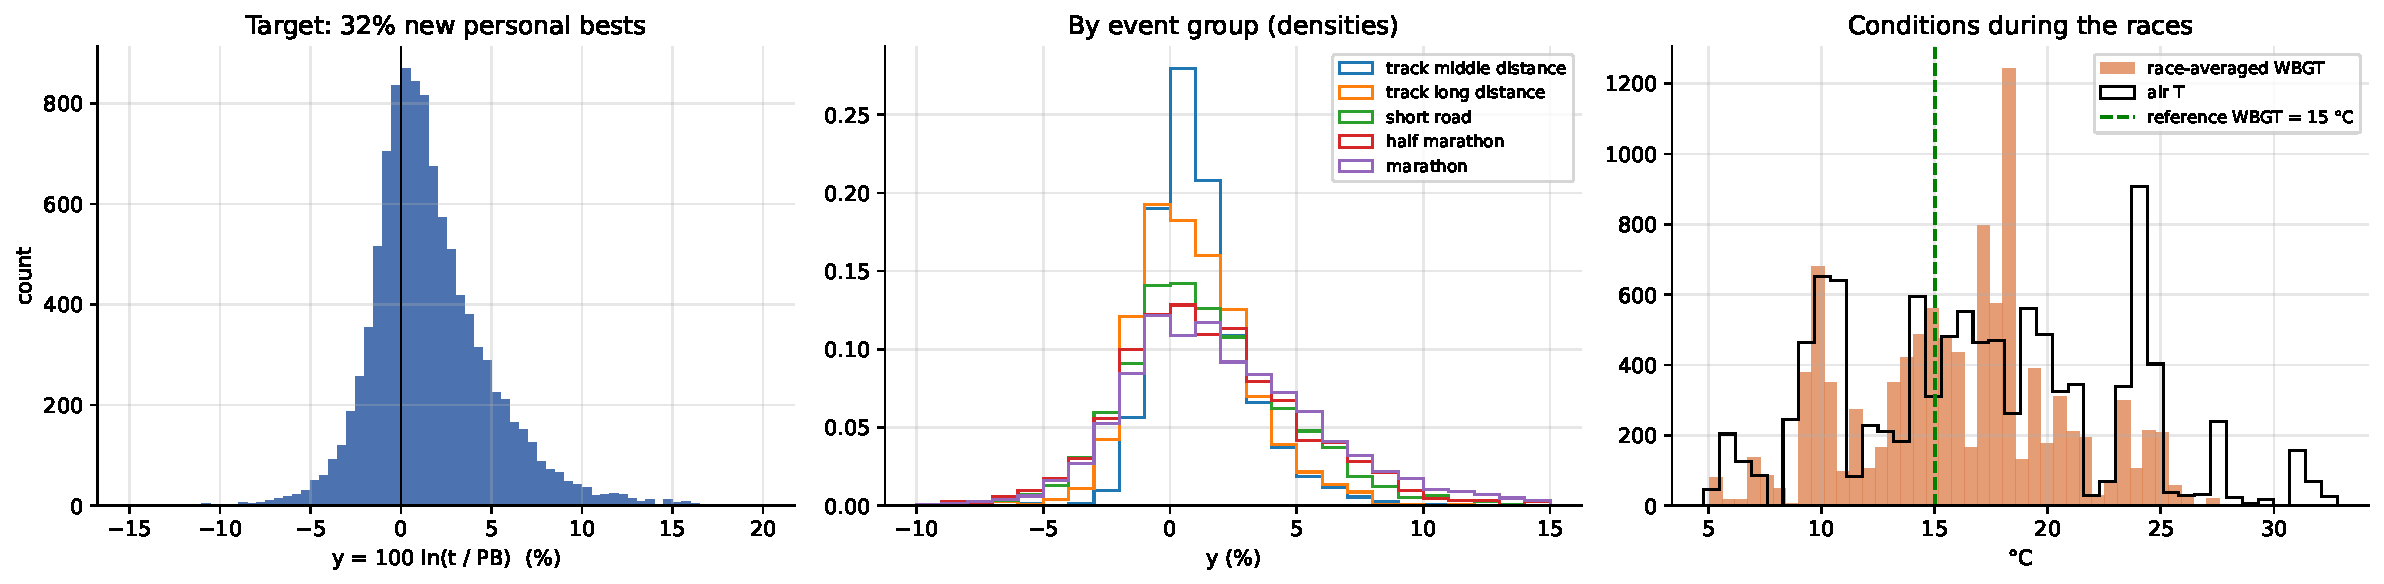
\includegraphics[width=\textwidth]{distributions}
\caption{Left, distribution of the target $y$ over the 10,398 performances of the analysis sample; center, densities
of $y$ by event group; right, distributions of the race-averaged WBGT and of air temperature, with the reference WBGT
of 15~°C.}
\label{fig:distributions}
\end{figure}

\paragraph{The shape of the target.} Of the 10,398 performances, 32\% are faster than the pre-race personal best
(figure~\ref{fig:distributions}). The median is 1.1\%, the mean 1.6\%, and the 5th and 95th percentiles are at
$-2.8$\% and $+7.5$\%. The distribution is right-skewed (skewness 0.87) and heavy-tailed (excess kurtosis 2.5): 13.5\%
of performances are more than 5\% above the personal best, against 1.2\% more than 5\% below. One can run much slower
than one's best, on a bad day, in a tactical race or when injured, or simply because the best is old; one rarely runs
much faster.

That $y$ is positive on average is expected and owes nothing to the weather. The personal best is the \emph{minimum}
of past performances: any given race is therefore on average slower than this minimum, and the gap is all the larger
as an athlete's performances are dispersed. This is what we observe: the mean grows with the dispersion, from 0.9 to
1.2\% on the track to 2.2\% in the marathon. The 32\% of personal bests come mostly from progressing athletes, who are
young or whose best is old or set over few races.

Dispersion grows with distance: the standard deviation of $y$ is 1.9~points in middle distance, 2.2 in track long
distance, 3.3 to 3.6 on the road and 4.0 in the marathon, that is, a variance four times larger in the marathon than in
middle distance. The data are therefore strongly \emph{heteroscedastic}. Middle distance is also the group most
concentrated around 0 and the most skewed (1.52): 800 to 1,500~m runners race often, their best is recent and close to
their current level, and only bad days take them away from it. Conversely, 21\% of marathon runners finish more than
5\% above their best. We drew two consequences from this: a quadratic loss will be dominated by errors on the road and
in the marathon, so that metrics must be read by event group and not only overall; and heavy tails make the squared
error sensitive to a few extreme poor performances, which makes the absolute error a useful complement. The gap
between sexes is small (mean 1.7\% for women and 1.6\% for men, standard deviations 3.5 and 3.2) and is partly
explained by the distribution across events.

\paragraph{The conditions covered.} The race-averaged WBGT ranges from 5 to 27.6~°C, with a median of 16.4~°C.
According to the ACSM thresholds, 12\% of performances take place below 10~°C, 53\% between 10 and 18~°C, 26\% between
18 and 23~°C, 9\% between 23 and 28~°C, and none above 28~°C. The ranges differ greatly by group. Track middle and long
distance, run at summer evening meetings around 8~p.m., never go below 13.5~°C, with a median of 18.3~°C in middle
distance. The half marathon and the marathon, run between 8:30 and 10~a.m. and in the intermediate seasons, range from
5 to 22~°C and from 6 to 26~°C, with medians of 10.3 and 14.2~°C.

\paragraph{Weather is a race-level variable.} The WBGT varies very little between runners of the same race: the gap
between the first and the last listed runner never exceeds 1.2~°C, with a median of 0.24~°C in the marathon. This is
again an effect of truncation: the lists keep only fast runners, who finish a few minutes apart. The information
available on the effect of weather therefore rests on 396 races, not on 10,398 rows. These races moreover have very
unequal sizes: 14 performances at the median, 293 at most (Lille 10~km), and the 20 largest races account for 32\% of
the rows. Yet these large races (the Valencia, Tokyo or Berlin marathons, the Boulogne half marathon) are run in cool
conditions, and hot races are smaller: 19\% of races have a WBGT above 23~°C, against 9\% of performances. An ordinary
regression, which weights each row equally, would therefore give much weight to a few cool marathons and little to
hot races. This observation will be at the heart of the validation protocol (section~\ref{sec:validation}) and of the
mixed models (section~\ref{sec:mixed}).

\paragraph{The composition of the WBGT.} The WBGT does not have the same composition across event groups. On the
track, evening meetings combine warm air (median temperature of 23.8~°C in middle distance), dry air (relative
humidity of 52\%) and a low sun (190~W/m²). Morning marathons combine cooler (13.2~°C), more humid (64\%) air and
strong radiation (430~W/m²). Two extreme examples reach the same WBGT by opposite routes: the 2026 Dessau meeting
(31.5~°C, 38\% humidity, 200~W/m², WBGT of 26.0~°C) and the 2026 Guiyang marathon (only 21.2~°C, but 73\% humidity and
540~W/m², WBGT of 25.8~°C). A model that saw only air temperature would rank these two races poorly. Conversely, it is
not obvious that the same WBGT has the same physiological effect whatever its composition;
section~\ref{sec:raw_weather} confronts the WBGT with the raw meteorological variables.

The \emph{drift during the race} is large over long distances: from the start to its maximum, the WBGT rises by a
median of 2.4~°C in the half marathon and 3.7~°C in the marathon, whereas it is zero on the track. The WBGT at the
start, often the only published value, therefore underestimates the stress endured, which justifies a posteriori the
use of the WBGT averaged over the race duration.

\begin{figure}[htbp]
\centering
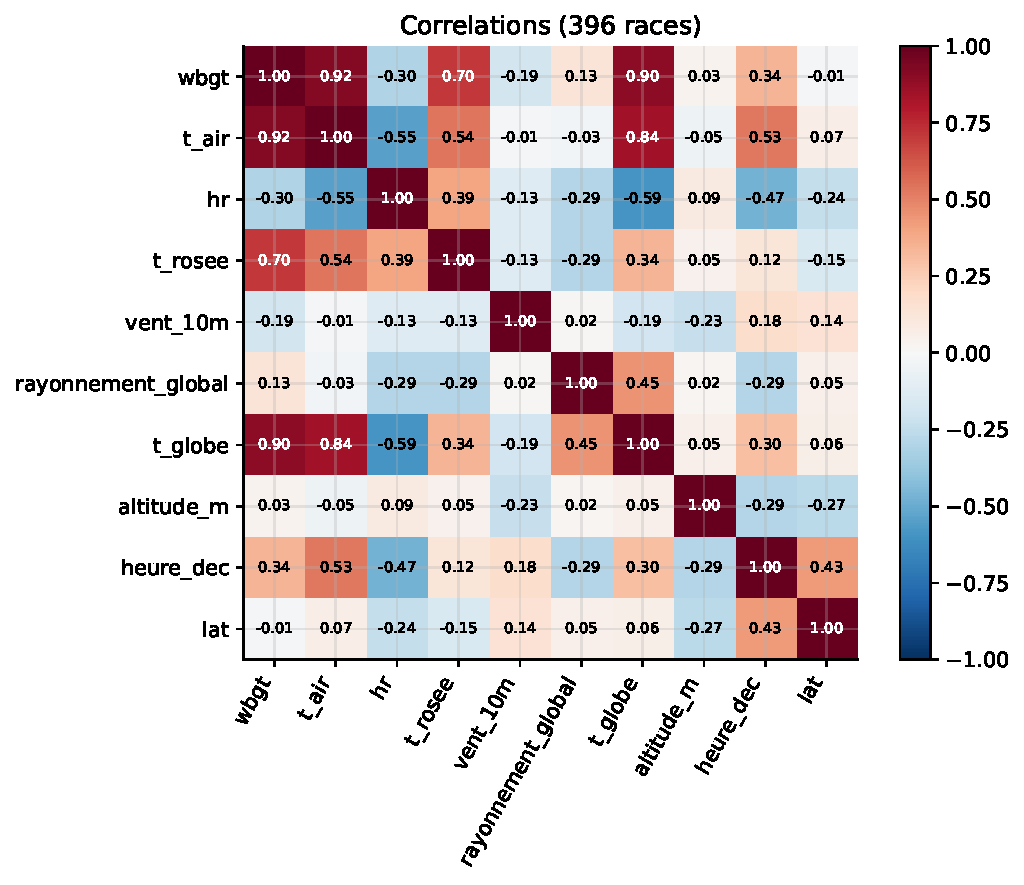
\includegraphics[width=0.56\textwidth]{correlations}
\caption{Pearson correlations between meteorological and context variables, computed on one row per race (396
races).}
\label{fig:correlations}
\end{figure}

\paragraph{Correlations between meteorological variables.} Since conditions are shared by all runners of a race, we
compute their correlations on one row per race: otherwise, a race of 293 runners would count 293 times. The Pearson
correlation coefficient between two variables $u$ and $v$,
\[
r = \frac{\sum_c (u_c - \bar u)(v_c - \bar v)}{\sqrt{\sum_c (u_c - \bar u)^2}\,\sqrt{\sum_c (v_c - \bar v)^2}}
\in [-1, 1],
\]
measures the strength of a linear relationship; $r = 0$ does not rule out a nonlinear relationship. The WBGT is highly
correlated with air temperature (0.92) and with globe temperature (0.90), more moderately with dew point (0.70), and
weakly with global radiation taken alone (0.13), because the hottest races are evening meetings, without sun
(figure~\ref{fig:correlations}). Relative humidity is anticorrelated with temperature ($-0.55$): this is the diurnal
cycle, during which relative humidity drops as the air warms up. ``Hot and humid'' combinations are therefore rare,
and it will be difficult to separate the effects of temperature and humidity from the data alone. This is one of the
merits of the WBGT: it combines these quantities through a physical model, instead of asking the statistical model to
learn this combination. Start time is linked to temperature (0.53) and to latitude (0.43): it mainly encodes the type
of meeting (track in the evening in Northern Europe, road in the morning) and will be a confounding factor to control
together with the event group. Altitude is almost uncorrelated with the WBGT (0.03), which in principle allows its
effect to be estimated separately; pressure, almost determined by altitude, adds nothing more. The extreme cities
illustrate the season more than the climate: Houston (January marathon and half marathon, 5.9~°C), Buenos Aires
(August half marathon, in the austral winter, 6.9~°C) or Cape Elizabeth (August 10~km, 26.5~°C). With one or two races
per city, these averages do not characterize the local climate.

\paragraph{Poorly represented combinations.} Several situations are rare or absent: the track in cool conditions
(below 16~°C), the half marathon in the heat (no race above 22~°C), the very hot marathon (only 8 races above 23~°C,
that is, 102 performances) and any extreme condition (WBGT above 28~°C). The crossing of event and heat is
unfavorable: half of the races above 23~°C are middle-distance races, where the expected effect of heat is the
weakest. For long distances, where the effect is the strongest, information on heat is scarce, and the effect in the
marathon in strong heat will rest on few races. Other factors vary little. Rain concerns only 37 races (more than
0.1~mm/h), and wind at 10~m never exceeds 6.3~m/s. Altitude is observed only on the road, in 18 races (168
performances, 1.6\% of the data) and 8 venues above 1,000~m, some of which are also hot (Guiyang, Kigali, Lanzhou): its
effect will be hard to separate from that of heat and of the field.

Three consequences for modeling emerge from this description. The event group, or the race duration, must enter the
model in interaction with the WBGT, since the WBGT ranges, the mean level of $y$ and its dispersion all differ by
group. Weather being a race-level variable, the unit of information is the race, which calls for grouped validation
and for a structure of race or course effects. Finally, the domain of validity of a tool based on these data is a
WBGT of 5 to 27~°C, without marked altitude or heavy rain; beyond it, the extrapolation must be flagged to the user.

\subsection{A first raw relationship, and Simpson's paradox}\label{sec:simpson}

The first idea, to get a feel for the effect of the WBGT, is to plot the mean of $y$ by WBGT class. We cut the WBGT into
classes of 3~°C. In class $b$, which contains $n_b$ performances, we compute the mean $\bar y_b$ and its
\emph{standard error}
\[
\mathrm{se}(\bar y_b) = \frac{s_b}{\sqrt{n_b}}, \qquad s_b^2 = \frac{1}{n_b - 1}\sum_{i \in b}(y_i - \bar y_b)^2 .
\]
The standard error is the standard deviation of the \emph{estimator} $\bar y_b$, that is, its variability from one
sample to another; it must not be confused with the standard deviation $s_b$ of the observations. The divisor
$n_b - 1$ makes $s_b^2$ unbiased, since the mean was estimated on the same data. By the central limit theorem,
$\bar y_b$ is approximately normal, hence the 95\% confidence interval $\bar y_b \pm 1.96\,\mathrm{se}(\bar y_b)$,
where $1.96$ is the $0.975$ quantile of the standard normal distribution. These error bars rest on a hidden
assumption: the formula $\Var(\bar y_b) = \sigma^2/n_b$ assumes independent observations. Since runners of the same
race share the weather and the course of the race, these bars are too narrow; we will measure this in
section~\ref{sec:dependence}.

A second difficulty has to do with the composition of the classes. The mean over all events in class $b$ is a weighted
mean of the means of each event group $e$:
\[
\bar y_b = \sum_e \pi_{e \mid b}\,\bar y_{e, b},
\]
where $\pi_{e \mid b}$ is the share of group $e$ in class $b$. If this composition changes from one class to another,
for example many middle-distance races in the hot classes and many marathons in the cool ones, the overall curve can
rise, fall or flatten even though each group shows a clear relationship. An aggregate trend can thus differ from, or
even reverse, the trends within each subgroup: this is \emph{Simpson's paradox}. Hence the value of reading the
curves by event group.

\begin{figure}[htbp]
\centering
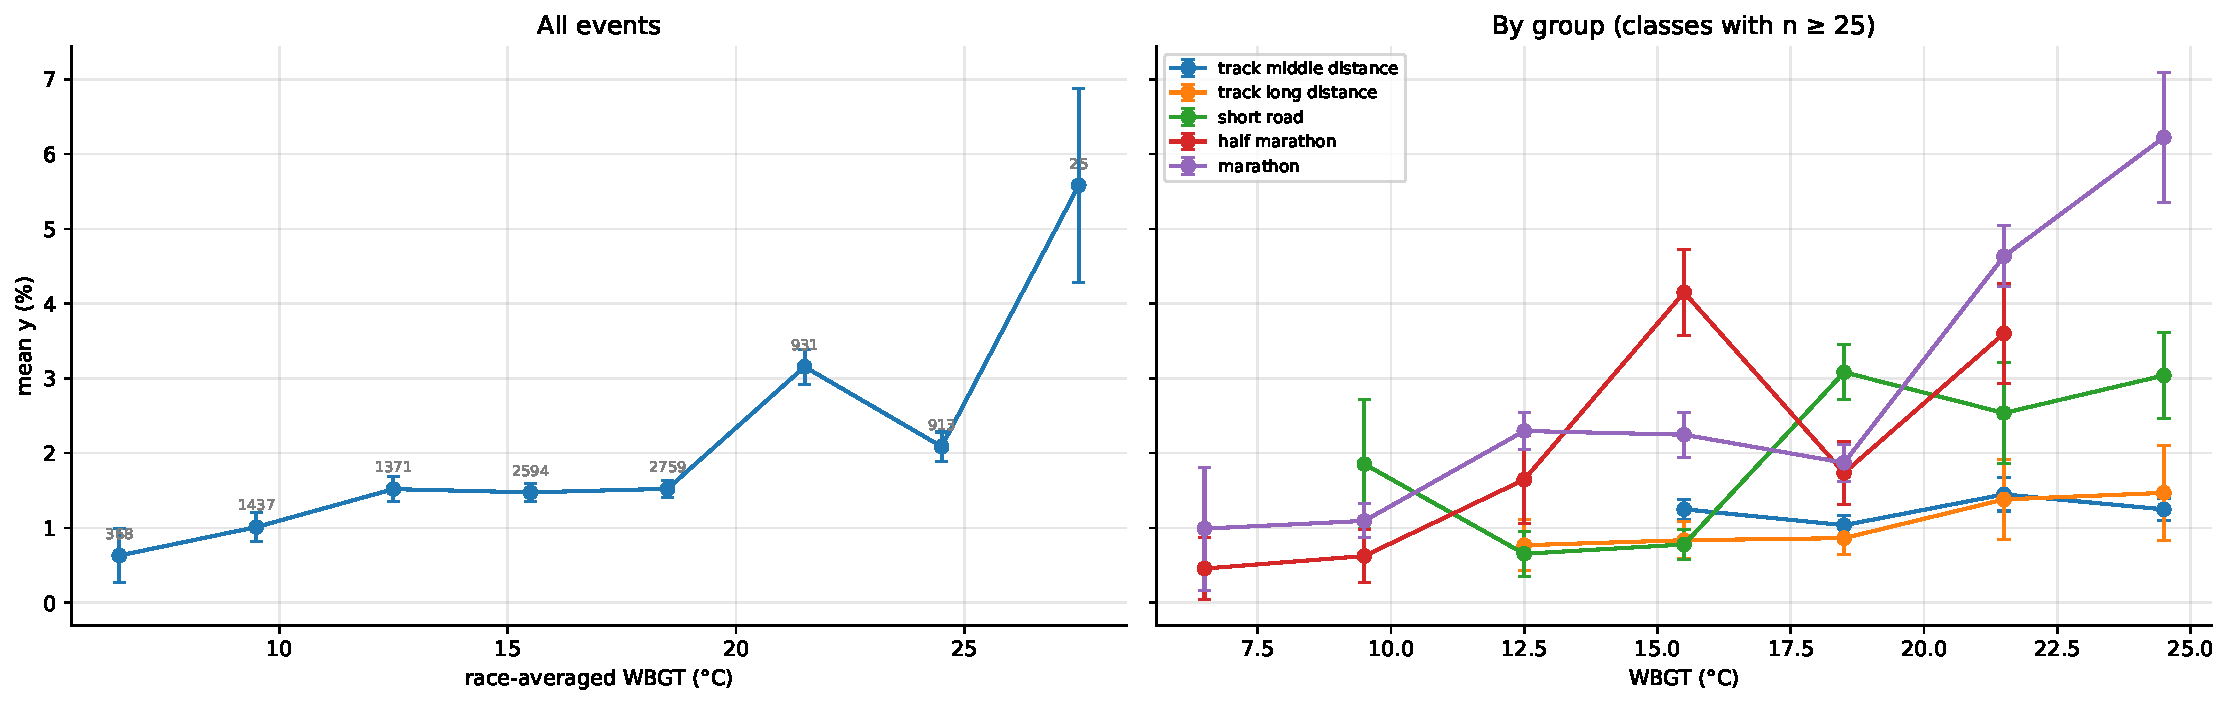
\includegraphics[width=\textwidth]{class_means}
\caption{Mean of $y$ by WBGT class of 3~°C, with 95\% confidence intervals computed under an independence assumption.
Left, all events together (sample sizes shown above the points); right, by event group, for classes with at least 25
performances.}
\label{fig:class_means}
\end{figure}

Figure~\ref{fig:class_means} illustrates exactly this phenomenon. All events together, $\bar y$ rises from 0.6\% (WBGT
of 5 to 8~°C) to 1.0\% (8 to 11~°C), stays around 1.5\% between 11 and 20~°C, then moves to 3.2\% between 20 and
23~°C. It then \emph{falls back} to 2.1\% between 23 and 26~°C, a class made up of 69\% track middle distance, before
reaching 5.6\% above 26~°C, on only 25 performances. By group, the contrast is clear. In the marathon, $\bar y$ is about
1\% up to 11~°C, 1.9 to 2.3\% between 11 and 20~°C, then 4.6\% between 20 and 23~°C and 6.2\% between 23 and 26~°C:
the slowdown is strong and convex, consistent with \citet{ely2007}. Track middle and long distance are almost flat
(0.8 to 1.5\%) over their whole range, from 12 to 26~°C. Short road races and the half marathon show irregular
profiles, such as the half-marathon peak between 14 and 17~°C (4.2\%); but each class there gathers only a handful of
races (2 to 20), and these means mix the effect of heat with that of the venue. The overall mean is therefore
misleading: its shape depends mostly on the event group that dominates each class.

\subsection{Confounding factors}\label{sec:confounding}

The WBGT is not randomly distributed. Hot races take place in certain countries (Southeast Asia, West Africa, the
Gulf) and in certain seasons, with different fields in level, age and proportion of athletes setting a personal best;
altitude is concentrated in a few cities. According to \eqref{eq:omitted_bias}, a confounding factor is dangerous only
if it is linked to the WBGT. We therefore measured, at the race level, the correlation between the WBGT and each
context variable. Each race $c$ receives a weight $w_c = n_c/\sum_{c'} n_{c'}$ proportional to its number of runners,
to reflect its weight in the individual data, and the weighted correlation reads
\[
r_w = \frac{\sum_c w_c\,(u_c - \bar u_w)(v_c - \bar v_w)}{\sqrt{\sum_c w_c\,(u_c - \bar u_w)^2}\,
\sqrt{\sum_c w_c\,(v_c - \bar v_w)^2}}, \qquad \bar u_w = \sum_c w_c\,u_c .
\]

\begin{figure}[htbp]
\centering
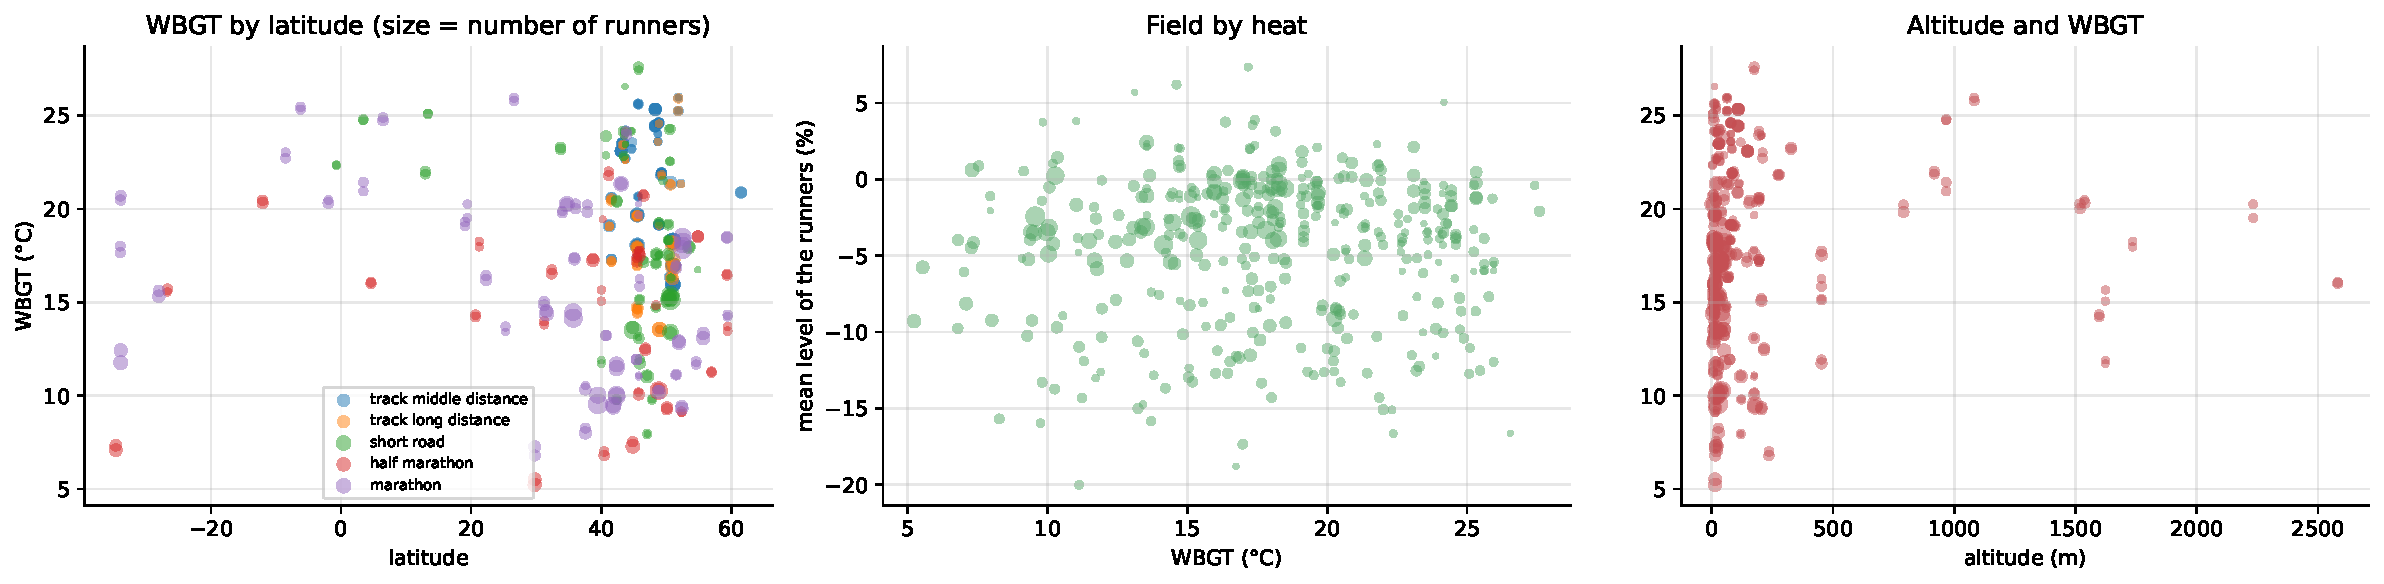
\includegraphics[width=\textwidth]{confounding}
\caption{Three potential confounding factors, at the race level (point size proportional to the number of runners).
Left, WBGT by latitude and event group; center, mean level of the runners by WBGT; right, WBGT by altitude.}
\label{fig:confounding}
\end{figure}

At the race level, the WBGT is correlated with the mean age of the runners ($-0.43$), with start time ($+0.42$), with
form ($-0.15$) and with altitude ($+0.13$), but hardly with level ($+0.05$, figure~\ref{fig:confounding}). Formula
\eqref{eq:omitted_bias} then makes it possible to anticipate the direction of the biases of a simple regression of
$y$ on the WBGT. The composition of events is the first of them: hot races are mostly track meetings (38 of the 75
races above 23~°C are middle-distance races), where heat matters little, and cool races are marathons and half
marathons; the average effect therefore underestimates that of the marathon and overestimates that of middle
distance. Next comes age: $y$ increases strongly with age (0.7\% before 23 years, 3.5 to 3.8\% after 38 years), because
an older runner's best is old; since hot races gather younger runners, $\beta_Z > 0$ and $\Cov(W, Z) < 0$, and the bias
is negative. Altitude works the other way: high-altitude venues (Kigali, Mexico City, Guiyang, Lanzhou) are also hot,
and hypoxia slows runners down, hence a positive bias if altitude is omitted. Country and course induce a bias of
unknown direction: the WBGT is high in the tropics (Jakarta, Chon Buri, Lagos, Cali) and at European summer meetings,
and these races also differ in profile, field and stakes. Finally, selection biases downward: in strong heat, some
runners give up, drop out or ``manage'' their race, and the truncation of the lists cuts off slow performances.

\subsection{Truncation: proof and remedy}\label{sec:truncation}

Let us return to the pitfall of truncation, which kept us busy for a long time. Consider two runners of the same
level, whose marathon best is 2:30, in a race that only lists men under 2:37. In cool weather, both finish between
2:30 and 2:35: they are under the threshold and appear in the results. With a high WBGT, the first runs 2:36 and
remains listed; the second, more affected by the conditions, runs 2:45, exceeds the threshold and disappears from the
results. Only the runner more resistant to heat therefore appears in the data. For athletes whose best is close to the
threshold, that is, the slowest of the list, we only observe in strong heat those who ran well relative to their
level: their mean slowdown is underestimated, and the effect of heat is biased toward zero.

To make this precise, let us model the situation. Suppose that, in the absence of truncation,
$y_i = \mu_i + \varepsilon_i$ with $\varepsilon_i \sim \mathcal{N}(0, \sigma^2)$, where $\mu_i = \E[y_i]$ is the
mean slowdown expected for athlete $i$ in the conditions of their race; an increase in WBGT increases $\mu_i$. Yet
$y_i$ is observed only if $y_i \leq m_i$, and the quantity actually observed on average is
$\E[y_i \mid y_i \leq m_i]$. Let $\varphi$ and $\Phi$ denote the density and the cumulative distribution function of
the standard normal distribution, and $a_i = (m_i - \mu_i)/\sigma$ the margin expressed in standard deviations. Since
$z\varphi(z) = -\varphi'(z)$,
\[
\E[\varepsilon \mid \varepsilon \leq \sigma a] = \frac{1}{\Phi(a)}\int_{-\infty}^a \sigma z\,\varphi(z)\,\dd z
= -\sigma\,\frac{\varphi(a)}{\Phi(a)},
\]
hence the expectation of a normal distribution truncated from above:
\begin{equation}\label{eq:truncation}
\E[y_i \mid y_i \leq m_i] = \mu_i - \sigma\,\Lambda(a_i), \qquad \Lambda(a) = \frac{\varphi(a)}{\Phi(a)},
\end{equation}
where $\Lambda$ is the inverse Mills ratio. If heat increases $\mu_i$ by $\delta$, the observed mean therefore increases
by only $\delta\,\partial_\mu \E[y \mid y \leq m]$. To compute this derivative, note that $a = (m - \mu)/\sigma$
depends on $\mu$, with $\partial a/\partial \mu = -1/\sigma$, and that, since $\varphi'(a) = -a\,\varphi(a)$,
\[
\Lambda'(a) = \frac{\varphi'(a)\,\Phi(a) - \varphi(a)^2}{\Phi(a)^2} = -\Lambda(a)\big(a + \Lambda(a)\big).
\]
It follows that
\begin{equation}\label{eq:attenuation}
\frac{\partial}{\partial \mu}\big[\mu - \sigma\Lambda(a)\big] = 1 + \Lambda'(a) = 1 - \Lambda(a)\big(a + \Lambda(a)\big).
\end{equation}
This factor lies between 0 and 1: it is also the ratio $\Var(y \mid y \leq m)/\sigma^2$, and the variance of a
truncated distribution is always smaller than that of the complete distribution. The estimated slope is therefore
\emph{attenuated}, all the more so as the margin $a$ is small. When the margin is large, truncation becomes
negligible: $\Lambda(a) \to 0$, the factor tends to 1 and the bias vanishes.

This analysis directly suggests the remedy: keep only the athletes whose margin to the threshold is sufficient,
$m_i \geq M$ for a fixed minimum margin $M$. For them, any slowdown up to $M$\% remains observable. It is essential
that this filter bear on the athlete's \emph{personal best} compared with the last listed time, and not on their
result of the day: it removes athletes close to the threshold, not those who ran poorly, and therefore does not itself
create selection on $y$. Its cost is that of a smaller sample of higher level. It reduces the bias without
eliminating it: a slowdown larger than the margin, or a dropout, remains invisible.

The data confirm the mechanism. Among the 4,425 valid performances whose margin is below 5\%, 63\% are personal bests,
against 32\% in the analysis sample: an athlete whose best is close to the last listed time appears only if they run
fast.

To measure the effect of the choice of $M$, we compared the slope of $y$ against the WBGT for several minimum margins
(0, 2, 5, 8, 10 and 12\%). If truncation biases toward zero, the slope must increase with $M$. The tool is the simple
linear regression $y = \beta_0 + \beta_1 W + \varepsilon$, where $\beta_1$ is the slope in points of $y$ per degree,
and $\varepsilon$ a random error with zero mean and variance $\sigma^2$. Least squares retain the values of
$(\beta_0, \beta_1)$ that minimize $S(\beta_0, \beta_1) = \sum_i (y_i - \beta_0 - \beta_1 W_i)^2$. The condition
$\partial S/\partial \beta_0 = 0$ gives $\hat\beta_0 = \bar y - \hat\beta_1\,\bar W$: the line goes through the mean
point. The condition $\partial S/\partial \beta_1 = 0$ then gives
$\sum_i (W_i - \bar W)(y_i - \bar y) = \hat\beta_1\sum_i (W_i - \bar W)^2$, hence
\[
\hat\beta_1 = \frac{\sum_i (W_i - \bar W)(y_i - \bar y)}{\sum_i (W_i - \bar W)^2}
= \frac{\widehat{\Cov}(W, y)}{\widehat{\Var}(W)} = r\,\frac{s_y}{s_W} .
\]
The slope combines the strength of the linear relationship $r$ and the ratio of the scales of the two variables.
Since $\sum_i (W_i - \bar W) = 0$, one can write $\hat\beta_1 = S_{WW}^{-1}\sum_i (W_i - \bar W)\,y_i$ with
$S_{WW} = \sum_i (W_i - \bar W)^2$: it is a linear combination of the $y_i$. With independent errors of variance
$\sigma^2$,
\[
\E[\hat\beta_1] = \beta_1, \qquad \Var(\hat\beta_1) = \frac{\sigma^2}{S_{WW}}, \qquad
\widehat{\mathrm{se}}(\hat\beta_1) = \frac{\hat\sigma}{\sqrt{S_{WW}}} .
\]
The standard error decreases when the data are more numerous, when the WBGT varies over a wider range and when the
noise is smaller. It remains to estimate $\sigma^2$, from the residuals $\hat\varepsilon_i = y_i - \hat\beta_0 -
\hat\beta_1 W_i$. These satisfy two constraints, $\sum_i \hat\varepsilon_i = 0$ and
$\sum_i W_i\,\hat\varepsilon_i = 0$, and vary freely only in a space of dimension $n - 2$, the number of \emph{degrees
of freedom}. One shows that $\E\big[\sum_i \hat\varepsilon_i^2\big] = (n - 2)\,\sigma^2$, hence the unbiased estimator
$\hat\sigma^2 = \sum_i \hat\varepsilon_i^2/(n - 2)$; dividing by $n$ would underestimate $\sigma^2$, since the line is
fitted as close as possible to the points. For large $n$, $\hat\beta_1$ is approximately normal, hence the 95\%
confidence interval $\hat\beta_1 \pm 1.96\,\widehat{\mathrm{se}}(\hat\beta_1)$.

\begin{figure}[htbp]
\centering
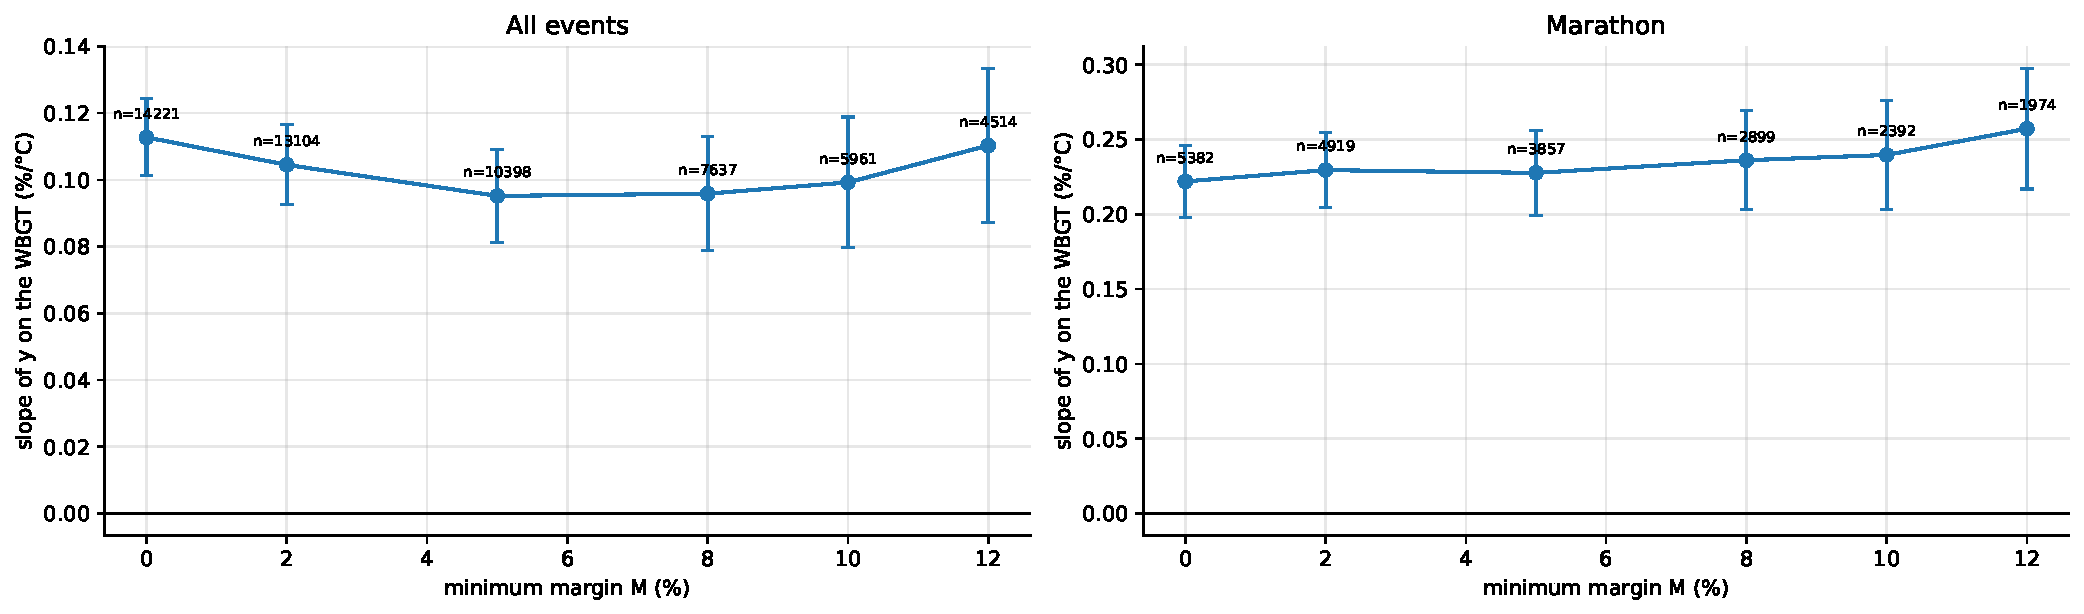
\includegraphics[width=\textwidth]{slopes_by_margin}
\caption{Slope of the simple regression of $y$ on the WBGT according to the minimum margin $M$ required, all events
together (left) and in the marathon (right), with 95\% confidence intervals computed under an independence
assumption. Sample sizes are shown above the points.}
\label{fig:slopes_margin}
\end{figure}

Three points guide the reading of the experiment. Without truncation, the slope would be roughly constant: the
subsample changes, not the true slope. A larger $M$ reduces the bias but removes data, so that the confidence interval
widens; this is a trade-off between bias and variance, and the sample also changes in nature, since it keeps only
faster athletes. Finally, the subsamples are nested (the one for $M = 12$ is included in the one for $M = 5$): the
slopes are highly correlated with one another, and overlapping intervals are not enough to conclude that two slopes
are equal.

The overall slope moves little with the margin (figure~\ref{fig:slopes_margin}): 0.113~point per degree without
filtering ($M = 0$, 14,221 performances), 0.095 for $M = 5$ and 0.110 for $M = 12$ (4,514 performances). In the
marathon alone, to avoid Simpson's paradox, it increases with $M$: 0.222, then 0.228 and 0.257~point per degree. This
is the expected direction: requiring a larger margin removes the races where attenuation is possible. The magnitude
remains modest, $+15$\% between $M = 0$ and $M = 12$, within the margins of uncertainty, whereas the sample is divided
by 2.7. We retained $M = 5$\% as a compromise, and we will return to this choice in section~\ref{sec:discussion} with
the final model. Two caveats are in order: the overall slope mixes events, and the intervals shown assume independent
performances. The next section shows that they are in fact about twice too narrow.

\subsection{A strong dependence structure}\label{sec:dependence}

Runners of the same race share the weather, the course of the race (pacemakers, tactics) and the field; editions of the
same course share its profile. We wanted to measure the share of the variance of $y$ common to runners of the same
race, the same meeting, the same course or the same venue. The natural tool is the \emph{intraclass correlation}.

Suppose the observations are divided into $G$ groups and write, for athlete $j$ of group $g$,
\begin{equation}\label{eq:random_effect}
y_{gj} = \mu + u_g + \varepsilon_{gj}, \qquad u_g \sim \mathcal{N}(0, \tau^2), \qquad
\varepsilon_{gj} \sim \mathcal{N}(0, \sigma^2),
\end{equation}
all independent. The effect $u_g$ is shared by all observations of the group (same weather, same race dynamics, same
course); $\varepsilon_{gj}$ is the part specific to the individual. Two runners of the same group share the same
$u_g$, hence
\[
\Var(y_{gj}) = \tau^2 + \sigma^2, \qquad \Cov(y_{gj}, y_{gj'}) = \Var(u_g) = \tau^2 \quad (j \neq j'), \qquad
\mathrm{ICC} = \Corr(y_{gj}, y_{gj'}) = \frac{\tau^2}{\tau^2 + \sigma^2} .
\]
The ICC has two equivalent readings: the share of total variance due to groups, and the correlation between two
observations of the same group. It is zero if groups play no role, and equals 1 if all observations of a group are
identical.

To estimate it with groups of unequal sizes, we use the analysis-of-variance estimator. With $N$ observations, $n_g$
observations in group $g$, $\bar y_g$ the group mean and $\bar y$ the overall mean, total variation decomposes into a
between-group part and a within-group part:
\[
\underbrace{\sum_g\sum_j(y_{gj}-\bar y)^2}_{\text{total}}
= \underbrace{\sum_g n_g(\bar y_g-\bar y)^2}_{\text{between groups}}
+ \underbrace{\sum_g\sum_j(y_{gj}-\bar y_g)^2}_{\text{within groups}} .
\]
Dividing each sum by its number of degrees of freedom, we define the mean squares and an effective group size $n_0$:
\[
\mathrm{MSB} = \frac{\sum_g n_g(\bar y_g - \bar y)^2}{G-1},\qquad
\mathrm{MSW} = \frac{\sum_g\sum_j (y_{gj} - \bar y_g)^2}{N-G},\qquad
n_0 = \frac{N - \sum_g n_g^2/N}{G-1} .
\]
Under model \eqref{eq:random_effect}, $\E[\mathrm{MSW}] = \sigma^2$ and $\E[\mathrm{MSB}] = \sigma^2 + n_0\,\tau^2$.
Within a group, indeed, $u_g$ is common to all and disappears from the deviations $y_{gj} - \bar y_g$, which contain only
individual noise; $N - G$ degrees of freedom remain, since $G$ means have been estimated. Group means, on the other
hand, vary for two reasons: the true differences between groups, of variance $\tau^2$, and sampling noise, of variance
$\sigma^2/n_g$. Expanding the expectation of the between-group sum gives
$(G - 1)\,\sigma^2 + \big(N - \sum_g n_g^2/N\big)\,\tau^2$, hence the factor $n_0$. If all groups have the same size
$n$, $n_0 = n$; if they are unbalanced, $n_0$ is smaller than the mean size $N/G$, because large groups bring less
information on $\tau^2$ than their size suggests. Equating each mean square to its expectation yields the
method-of-moments estimator
\[
\hat\sigma^2 = \mathrm{MSW}, \qquad \hat\tau^2 = \frac{\mathrm{MSB}-\mathrm{MSW}}{n_0}, \qquad
\widehat{\mathrm{ICC}} = \frac{\mathrm{MSB} - \mathrm{MSW}}{\mathrm{MSB} + (n_0 - 1)\,\mathrm{MSW}} .
\]
When the true ICC is close to 0, MSB can be smaller than MSW by chance, and the estimator slightly negative; we do not
truncate it at 0, which would introduce an upward bias.

The practical consequence of the ICC shows in the variance of a mean. For $n$ observations from the same group,
pairwise correlated with correlation $\rho$ and with variance $\sigma_t^2 = \tau^2 + \sigma^2$,
\[
\Var(\bar y) = \frac{1}{n^2}\Big[n\,\sigma_t^2 + n(n-1)\,\rho\,\sigma_t^2\Big] = \frac{\sigma_t^2}{n}\,
\big[1 + (n - 1)\rho\big].
\]
The factor $\mathrm{deff} = 1 + (\bar n - 1)\rho$, called the \emph{design effect} \citep{kish1965}, measures by how
much correlation multiplies the variance compared with independent observations. The \emph{effective sample size}
$N/\mathrm{deff}$ is the number of independent observations that would bring the same information.

The result was one of the surprises of the study. About 17\% of the variance of $y$ is common to runners of the same
race (ICC of 0.18), the same meeting (0.17), the same course (0.17) or the same venue (0.16). These values are almost
equal: most of what is shared is already shared at the venue level (weather, course, field, the day's conditions),
and almost nothing is gained by going down to the race. With 26 performances per race on average, the design effect is
about $1 + 25 \times 0.18 \approx 5.5$: the 10,398 performances are worth only about 1,900 independent observations,
and only 396 distinct weather situations. Four consequences follow: confidence intervals computed under an
independence assumption are about $\sqrt{5.5} \approx 2.3$ times too narrow; random validation folds would let venue
effects leak; confidence intervals will have to resample venues, not rows; and a model with a random race effect is
natural.

\section{A leak-proof validation protocol}\label{sec:validation}

The final tool will be used to estimate the effect of weather conditions in a city and a race that have never been
observed. The evaluation protocol must reproduce this situation: a model is judged only on data absent from its
training, and these data must be as independent of it as those of a real use will be. The dependence structure
uncovered in section~\ref{sec:dependence} makes this requirement decisive.

\subsection{Information leakage and grouping by venue}\label{sec:leakage}

Let $\ell$ denote a loss function and $f$ a predictor. The error measured on a validation set is an unbiased estimate
of the generalization risk $\mathcal{R}(f) = \E[\ell(f(x), y)]$ only if the training and validation sets are
independent. When information shared between the two sets is available at evaluation time but will not be in real
use, the measured error is too optimistic: this is called \emph{information leakage}. Three dependence structures are
at stake here. Weather and random events are first shared within a race and a meeting: all runners of a race
experience almost the same WBGT and the same race dynamics (pacemakers, tactics, headwind in the home straight). A
random split of the rows would place the same race on both sides, and the model could associate the day's random
events with a WBGT value and be rewarded for this overfitting. The speed of a course is then shared between its
editions: Boston remains hilly from one year to the next, Valencia remains fast. If the 2023 edition is in training
and the 2026 edition in validation, the model can recognize the course, through its altitude and typical conditions,
and benefit from it without having learned anything about the effect of weather. Athletes, finally, may appear
several times; this is rare in our data, and their level is already absorbed by the personal best.

We therefore grouped the data at the most encompassing level, the venue: all races, editions and events of the same
city are placed on the same side of every split. This cautious choice costs almost nothing, since the venue ICC (0.16)
is close to that of the race (0.18).

About 20\% of the venues are first set aside to form the \emph{test set}. Hot conditions being rare, the draw is
stratified: venues are divided into three climate terciles according to their mean WBGT, then
$\lceil 0.2\, n_{\text{tercile}} \rceil$ venues are drawn at random in each tercile, where $n_{\text{tercile}}$ is the
number of venues in the tercile. The test set thus contains hot, cool and intermediate venues. It is used \emph{only
once}, for the final evaluation (section~\ref{sec:comparison}): choosing a model or a hyperparameter on the test set
would make its error optimistic.

On the remaining venues, models and their hyperparameters are chosen by \emph{cross-validation} with $K = 5$ folds.
For each fold $k$, a model is trained on the other four folds, denoted $\mathcal{A}_k$, then evaluated on fold $k$,
denoted $\mathcal{V}_k$; the risk is estimated by the mean of the $K$ errors. Each fold is made up of whole venues. To
balance the folds in number of performances, venues are assigned greedily: they are sorted by decreasing size, then
each is placed in the least filled fold.

The resulting test set contains 21 venues and 2,355 performances (23\% of the data). It covers the range of climates
well, with a mean WBGT per venue ranging from 9.5~°C (Chicago marathon) to 26.5~°C (Cape Elizabeth): cool venues
(Chicago, Valencia, Auxerre, Cholet), intermediate ones (Annecy, Brest, Cape Town) and hot ones (Ordizia, Smederevo,
Chon Buri, Jakarta). Two venues weigh heavily in it: Portland (686 track performances) and Valencia (415 marathon
performances). The 79 remaining venues (8,043 performances) form five balanced folds of 1,607 to 1,611 performances,
that is, 14 to 17 venues each. No venue, course, meeting or race identifier is shared between training and validation.
By comparison, a random split of the rows, with 80\% for training, would share 77 of the 79 venues, 119 courses, 105
meetings and 247 races between training and validation: almost all the dependence structures identified would be
present on both sides. Section~\ref{sec:raw_weather} will measure the cost of this leakage.

\subsection{Evaluation metrics}\label{sec:metrics}

For $n$ observations $y_i$ and their predictions $\hat y_i$, we use three metrics:
\[
\mathrm{RMSE} = \sqrt{\frac1n\sum_i (y_i - \hat y_i)^2},\qquad
\mathrm{MAE} = \frac1n\sum_i |y_i - \hat y_i|,\qquad
R^2 = 1 - \frac{\sum_i (y_i - \hat y_i)^2}{\sum_i (y_i - \bar y)^2}.
\]
The root mean squared error (RMSE) is expressed in the unit of $y$, in percentage points, and strongly penalizes large
errors. It corresponds to the squared loss, whose minimizer is the conditional expectation $\E[y \mid x]$: it is our
main metric, consistent with the loss used by the models. The mean absolute error (MAE) corresponds to the absolute
loss, whose minimizer is the conditional median; it is more robust to extreme values, and is a useful complement for
a skewed, heavy-tailed and heteroscedastic target. The coefficient $R^2$ measures the share of the variance of $y$
explained by the model, by comparison with the constant prediction $\bar y$ computed on the evaluated sample. Out of
sample, it can be negative: the model then does worse than this mean. Even the constant model obtains a slightly
negative validation $R^2$, since it predicts the training mean and not that of the evaluated fold.

We expected modest $R^2$ values. Most of the variance of $y$ comes from variability from one race to another and from
one runner to another (form on the day, tactics, age of the personal best), which weather explains only in part. For
the final tool, the quality of the \emph{estimate of the effect} of heat, that is, of the degradation curve, matters
at least as much as the accuracy of individual predictions.

\subsection{Derived variables and the Mundlak decomposition}\label{sec:mundlak}

Three variables were added. They are computed within a row or within a course; since a course belongs to a single
venue, their computation introduces no leakage between folds. The first is the logarithm of the expected race
duration: the effect of heat grows with the duration of the effort, and the logarithm puts on the same scale an
800~m (about two minutes) and a marathon (about 150 minutes). The second is the \emph{useful altitude}
$\max(0,\ \text{altitude} - 500)/1000$, in kilometers above 500~m: this hinge function expresses the physiological
assumption of a negligible effect of hypoxia below 500~m and a linear one above.

The third addresses confounding between venues. Let $\bar W_g$ denote the mean WBGT of course $g$, over all editions
and all runners. Any WBGT decomposes as
\begin{equation}\label{eq:mundlak}
W_{gj} = \underbrace{\bar W_g}_{\text{between courses}} + \underbrace{(W_{gj} - \bar W_g)}_{\text{within course}} .
\end{equation}
The within-course component varies from one edition to the next, or between fast and slow runners of the same race
who do not run during the same hours: it compares a course with itself, and remains sheltered from differences
between courses. The between-course component, on the contrary, compares different courses and remains exposed to the
confounding factors of section~\ref{sec:confounding}. Introducing $\bar W_g$ as an additional regressor allows the
WBGT coefficient to capture only the within-course effect \citep{mundlak1978}; we will see its formal justification in
section~\ref{sec:which_estimator}.

This decomposition revealed a serious limitation of the data: the standard deviation of the WBGT is 4.52~°C over the
whole data set, but only 1.04~°C within a course. Within-course variation thus represents only about 5\% of the WBGT
variance ($1.04^2/4.52^2 \approx 0.05$). Most of the information on heat comes from comparisons between venues,
exposed to confounding; an estimate based on within-course variation alone will be better protected from these
biases, but will rest on little variation and will have to be extrapolated to describe a 10~°C difference. In
addition, altitude above 1,000~m concerns only 168 performances, in 8~venues, and missing values are limited to age
(9.2\%) and form (45.1\%, for lack of a pre-race season's best).

\subsection{Preprocessing learned on the training set only}\label{sec:preprocessing}

The models operate on a numerical matrix $X \in \mathbb{R}^{n \times p}$. All preprocessing parameters (medians, means,
standard deviations, categories) are learned on $\mathcal{A}_k$ only, then applied as such to $\mathcal{V}_k$ or to the
test set: estimating them on the whole data set would be a leak, since the preprocessing would ``know'' the validation
venues. Missing values are imputed by the training median, robust to extreme values, and a missing-value indicator is
added, because the absence of a value can be informative: an athlete without a pre-race season's best has often not
run the event earlier in the year. Variables are finally standardized, $z = (x - \bar x)/s$. Standardization is
necessary for the ridge penalty, which depends on the scale of the coefficients, and eases the optimization of neural
networks; it is useless for trees, which are invariant under monotone transformations of the variables.

Each category of a categorical variable seen in training receives an indicator column (\emph{one-hot} encoding); an
unknown category produces a row of zeros. If all categories are encoded and the model has an intercept, the sum of the
indicators equals the constant column: $X$ is no longer of full rank and $X^\top X$ is not invertible. When necessary,
we therefore drop one so-called reference category, against which the other coefficients measure the difference.
Applied to the context variables, this preprocessing produces 15 columns: 6 numerical variables, 2 missing-value
indicators, 5 event groups and 2 sexes.

\subsection{Cross-validation and its variability}\label{sec:cv}

Cross-validation is a generic procedure: for each fold $k$, a new model is created, so that no information passes from
one fold to another, trained on $\mathcal{A}_k$ then evaluated on $\mathcal{V}_k$. The procedure also keeps the
\emph{out-of-fold predictions}: each training performance receives the prediction of a model that did not see it,
which makes it possible to analyze errors over the whole training data.

The constant model, which predicts the mean of $y$ on the training set, provides the first benchmark. Its
cross-validated RMSE is 3.30 on average, but varies a lot from one fold to another: from 2.65 on fold~0 to 3.67 on
fold~1. The standard deviation across folds (0.43) gives a standard error of the mean of about
$0.43/\sqrt5 \approx 0.19$. This variability sets the scale of the comparisons to come: a difference of a few
hundredths of RMSE between two models will not be significant. Since the folds are shared by all models, comparisons
will have to be made fold by fold, a difficult fold weighing on all models at once. The $R^2$ values of the constant
model are slightly negative, from $-0.017$ to $-0.0001$, as expected.

\section{First models: linear regressions}\label{sec:linear}

Before turning to flexible models, we established simple benchmarks. They answer two questions: what share of the
variance of $y$ is predictable on a new venue, and what share of this predictability is due to weather rather than to
the athletes' profile? They also provide a first estimate of the effect of heat, which section~\ref{sec:confounding}
showed to be exposed to several biases.

\subsection{Naive models}\label{sec:naive}

Two models without any explanatory variable serve as a floor. The constant model predicts the mean of $y$ on the
training set; any useful model must do better. The group-mean model predicts the mean of $y$ in the event $\times$ sex
cell of the performance, and the overall mean for a cell absent from training: it tests whether the mean level of each
group alone transfers to new venues.

The constant model obtains a cross-validated RMSE of 3.300, and the group-mean model 3.303: knowing the event and the
sex brings nothing on average. The fold-by-fold detail is instructive. The group means do better on three folds, by up
to $0.10$ on fold~0, and worse on the other two, by up to $0.15$ on fold~1. The differences in mean $y$ between groups,
of the order of one point, are small compared with the variability from one venue to another, and means learned on
some venues do not transfer to others: estimating ten means adds estimation variance without transferable
information.

\subsection{Ordinary least squares and ridge regression}\label{sec:ridge}

A column of ones, the intercept, is added to $X$, and we look for the coefficients $w$ that minimize
$\mathcal{L}(w) = \lVert y - Xw\rVert^2$. The gradient $\nabla\mathcal{L}(w) = -2X^\top(y - Xw)$ vanishes for the
\emph{normal equations}
\[
X^\top X\,\hat w = X^\top y, \qquad \text{that is,} \qquad \hat w = (X^\top X)^{-1}X^\top y
\quad \text{if } X^\top X \text{ is invertible.}
\]
Geometrically, $X\hat w$ is the orthogonal projection of $y$ onto the space spanned by the columns of $X$, and the
residual $y - X\hat w$ is orthogonal to each of them. If columns are collinear, $X^\top X$ is not invertible and there
are infinitely many solutions; we then retain the minimum-norm solution $\hat w = X^+ y$, where $X^+$ is the
Moore--Penrose pseudo-inverse, computed by singular value decomposition.

Ridge regression, or Tikhonov regularization, adds to the loss a penalty on the size of the coefficients, without
penalizing the intercept $b$:
\[
\mathcal{L}(b, w) = \frac1n\sum_i (y_i - b - x_i^\top w)^2 + \lambda\lVert w\rVert^2 .
\]
The intercept sets the mean level of $y$, which has no reason to be close to 0: penalizing it would bias all
predictions. Setting the derivative with respect to $b$ to zero gives $\hat b = \bar y - \bar x^\top \hat w$.
Substituting, the problem only involves the centered data $X_c = X - \mathbf{1}\bar x^\top$ and
$y_c = y - \bar y\,\mathbf{1}$, and setting the gradient with respect to $w$ to zero leads to
\[
\hat w = (X_c^\top X_c + n\lambda I)^{-1}X_c^\top y_c,\qquad \hat b = \bar y - \bar x^\top \hat w.
\]
The matrix $X_c^\top X_c + n\lambda I$ is positive definite as soon as $\lambda > 0$: the solution always exists, even
with collinear columns. The effect of the penalty can be read on the singular value decomposition $X_c = UDV^\top$,
with columns $u_j$ and singular values $d_j$: the prediction reads
\[
X_c\hat w = \sum_j u_j\, \frac{d_j^2}{d_j^2 + n\lambda}\, u_j^\top y_c .
\]
Each direction of the variable space is shrunk by the factor $d_j^2/(d_j^2 + n\lambda) \in (0, 1)$: low-variance
directions, poorly determined by the data and unstable under least squares, are the most attenuated. Ridge accepts a
bias, coefficients pulled toward 0, in exchange for a lower variance. Two consequences will matter to us: the penalty
depends on the scale of the variables, hence the standardization; and, faced with two nearly collinear variables,
ridge tends to split the effect between them, since for a given sum $w_1 + w_2$, $w_1^2 + w_2^2$ is minimal when
$w_1 = w_2$.

\subsection{A polynomial basis for the WBGT}\label{sec:polynomial}

Figure~\ref{fig:class_means} suggests a nonlinear relationship between WBGT and performance, at least in the
marathon. To represent it in a model linear in its parameters, we replace the WBGT $W$ by the polynomial basis
\[
\psi(W) = \big(z, z^2, \dots, z^D\big), \qquad z = \frac{W - W_{\text{ref}}}{5},
\]
of degree $D$, where $5$~°C is a fixed scale. Centering and scaling before raising to a power avoids columns of very
different orders of magnitude ($25^3 \approx 15{,}600$ versus $25$), which would make $X^\top X$ ill-conditioned. The
center and scale are fixed a priori, since if estimated on the data they would change from one fold to another; the
power 0 is excluded, the intercept being handled by the model. The WBGT terms can also interact with the event group,
which allows the curve to differ from one group to another.

\subsection{What the linear models taught us}\label{sec:linear_results}

We compared three families of models in cross-validation by venue: least squares on the WBGT alone, which reproduce
the simple regression of section~\ref{sec:truncation}; polynomial ridge on the WBGT alone, with a degree
$D \in \{1, 2, 3, 4\}$ and $\lambda \in [10^{-3}, 10]$ chosen by cross-validation; and the full ridge, which adds to the
WBGT (of degree $D \le 3$) the control variables (level, age, form, duration, altitude, time, wind, rain, event group,
sex), with or without interactions between WBGT and event group, and with or without the Mundlak term, that is, 48
configurations.

To summarize the effect of heat according to a model $f$, we use the mean effect of a 10~°C increase in WBGT above the
reference,
\[
\overline{\Delta}_{10} = \frac1n \sum_i \Big[ f(x_i \mid W = W_{\text{ref}} + 10) - f(x_i \mid W = W_{\text{ref}}) \Big],
\]
all other variables keeping their observed values. For a linear model of degree 1 without interaction, this is exactly
ten times the WBGT slope.

\paragraph{The WBGT alone brings almost nothing in prediction.} Least squares on the WBGT obtain an RMSE of 3.301,
slightly worse than that of the constant model (3.300). The best polynomial ridge ($D = 1$, $\lambda = 1$) reaches
3.291, a gain of only 0.009, and the whole grid lies between 3.291 and 3.323. Degrees 2 to 4 only match degree 1 with
a strong penalty, which brings the polynomial back toward a straight line: nothing justifies a curvature at this
stage. This result does not imply that heat has no effect. The variance of $y$ is dominated by differences between
races and between runners, and the raw effect of the WBGT is blurred by the composition of events and by confounding
factors; a model that only sees the WBGT cannot separate these contributions.

\paragraph{Control variables change everything.} With the controls, the RMSE drops from 3.30 to 2.988 and the
validation $R^2$ reaches 0.18: about one fifth of the variance of $y$ becomes predictable on a new venue. This gain
comes from the athletes' profile (age, level, form) and the type of event much more than from the weather, whose
isolated contribution to prediction is nil. The best configuration is a polynomial of degree 3 with interactions
between WBGT and event group, without the Mundlak term, with $\lambda = 0.1$. But the eight best configurations lie
within 0.012 of RMSE, and the simplest configuration (degree 1, without interactions) is only 0.008 away from the best.
These differences are more than ten times smaller than the standard error across folds: cross-validation cannot
separate them, and retaining the minimum amounts to choosing partly at random, here the most complex model. Yet a
degree-3 polynomial specific to each event group extrapolates poorly outside the observed range: a WBGT of 25~°C is
beyond the data in the half marathon. This observation led us to adopt, in section~\ref{sec:mixed_cv}, a selection
rule that favors the simplest model among those that are statistically equivalent. The Mundlak term, for its part,
changes nothing in prediction (2.990 versus 2.988).

\paragraph{The effect of heat triples with the controls.} The mean effect of a 10~°C increase goes from 0.88~point
(least squares on the WBGT alone) to 2.50~points with controls and interactions, and to 2.65~points with the Mundlak
term. The controls correct the biases identified in section~\ref{sec:confounding}, in particular the downward bias due
to age. The interactions above all allow the effect to differ by event, instead of imposing a common slope dominated by
middle distance, where heat matters little. The computed effect nevertheless remains an average over all training
performances, and it includes cubic extrapolations for groups whose WBGT range does not reach 25~°C.

The Mundlak term gives a slightly stronger effect (2.65 versus 2.50). With $\bar W_g$ as a regressor, the WBGT
coefficient measures only the within-course effect: this effect is thus not weaker than the overall effect, which
suggests that the confounding between courses that remains once the controls are introduced does not inflate the
estimate. This reading calls for two caveats. The WBGT and its course mean are correlated at 0.97, and the ridge
penalty tends to split the effect between two such collinear variables: the within-course coefficient therefore
depends partly on $\lambda$. More generally, the penalty shrinks effects: the polynomial ridge on the WBGT alone, with
$\lambda = 1$, gives only 0.44~point, half as much as least squares. The $\lambda$ that optimizes prediction is not the
one that best estimates an effect. We therefore needed to estimate the effect of heat without a penalty, while
accounting for the dependence between runners of the same race: this is the purpose of mixed-effects models.

\section{Accounting for dependence: mixed-effects models}\label{sec:mixed}

The linear models of the previous section treat each performance as an independent observation. Yet 16 to 18\% of the
variance of $y$ is common to runners of the same race, the same course or the same venue, and weather is in practice
a race-level variable. Ignoring this structure raises three problems. The first is weighting: since each performance
counts equally, a race of 293 runners weighs 293 times more than a single-runner race in the estimate of the WBGT
effect, although it brings only one weather situation; and the twenty largest races, which gather about a third of
the performances, are mostly cool. The second is precision: the usual standard errors assume independent
observations and are too optimistic. The third is confounding between groups: if hot courses differ from the others
for unmeasured reasons (profile, field, organization), the estimated effect mixes heat with these differences.
Mixed-effects models directly address the first two problems, and we will see that they also make it possible to
tackle the third.

\subsection{The random-intercept model}\label{sec:random_intercept}

The model extends that of section~\ref{sec:dependence} by replacing the constant $\mu$ with a linear part:
\begin{equation}\label{eq:mixed}
y_{gj} = x_{gj}^\top\beta + u_g + \varepsilon_{gj},\qquad u_g \sim \mathcal N(0, \tau^2),\qquad
\varepsilon_{gj}\sim\mathcal N(0,\sigma^2),
\end{equation}
where $g$ indexes a group (a race or a course) and $j$ the $n_g$ runners of this group. The part $x_{gj}^\top\beta$ is
called the \emph{fixed-effects} part: its parameters are common to the whole population (effect of WBGT, age, level).
The \emph{random effect} $u_g$ is a shift common to all runners of the group. For a race, it represents the pace of the
pack, the pacemakers, the tactics or the wind in the home straight; for a course, the profile, the turns or the
surface, shared by all its editions. Since athletes hardly repeat and their level is absorbed by the personal best, it
is the group, not the athlete, that carries the useful shared effect. The deviation $\varepsilon_{gj}$ is specific to
the runner: form on the day, age of the personal best.

The assumptions are as follows: the $u_g$ and the $\varepsilon_{gj}$ are independent of each other and from one group
to another; their variances $\tau^2$ and $\sigma^2$ are the same for all groups; and above all, $u_g$ is independent of
the variables $x_{gj}$. This last assumption, called \emph{exogeneity}, is the most fragile; we return to it in
section~\ref{sec:which_estimator}.

Why a ``random'' effect? One could add one indicator per race, that is, race fixed effects. This would add nearly 300
parameters, poorly estimated for small races and useless for predicting a new race, whose effect is unknown by
definition. The mixed model replaces these parameters with a single one, the \emph{variance} $\tau^2$ of the group
effects: it describes the population of races rather than each race. The ratio $\tau^2/(\tau^2+\sigma^2)$ becomes a
\emph{conditional} ICC: the share of variance common to the group that remains once the athletes' profile has been
taken into account.

Two runners of the same group share $u_g$, hence $\Var(y_{gj}) = \tau^2 + \sigma^2$ and
$\Cov(y_{gj}, y_{gj'}) = \tau^2$ for $j \neq j'$. For a group of three runners, the covariance matrix of
$y_g = (y_{g1}, y_{g2}, y_{g3})^\top$ reads
\[
V_g = \begin{pmatrix} \tau^2+\sigma^2 & \tau^2 & \tau^2 \\ \tau^2 & \tau^2+\sigma^2 & \tau^2 \\
\tau^2 & \tau^2 & \tau^2+\sigma^2 \end{pmatrix} = \tau^2\,\mathbf 1\mathbf 1^\top + \sigma^2 I_3 ,
\]
and in general, for a group of $n_g$ runners,
\begin{equation}\label{eq:Vg}
V_g = \sigma^2\big(I_{n_g} + \gamma\,\mathbf 1\mathbf 1^\top\big), \qquad \gamma = \frac{\tau^2}{\sigma^2},
\end{equation}
where $\mathbf 1$ is the vector of $n_g$ ones. The ratio $\gamma$ of the group variance to the individual variance is
the only covariance parameter to estimate in addition to $\sigma^2$. Since the groups are independent, the covariance
matrix $V$ of all the data is block diagonal, with one block $V_g$ per group.

\subsection{From ordinary to generalized least squares}\label{sec:gls}

Under the exogeneity assumption, the total error $u_g + \varepsilon_{gj}$ still has zero mean given $x$: ordinary least
squares remain unbiased. But the Gauss--Markov theorem, which guarantees that they are the most precise linear unbiased
estimators, assumes uncorrelated errors with equal variance, which is no longer the case. The 293 runners of the same
race share the same $u_g$: their deviations from the line are not 293 independent pieces of information, since the
common part $u_g$ does not average out when runners are added. Ordinary least squares therefore overestimate the
information brought by large races.

When the covariance $V$ of the errors is known, the residual sum of squares is replaced by a distance that accounts
for the correlations. The \emph{generalized least squares} (GLS) estimator is
\[
\hat\beta_{\text{GLS}} = \arg\min_\beta\ (y - X\beta)^\top V^{-1} (y - X\beta) = (X^\top V^{-1}X)^{-1}X^\top V^{-1}y .
\]
Aitken's theorem, or generalized Gauss--Markov theorem, establishes that it is the linear unbiased estimator of
minimum variance \citep{aitken1935}. Its interpretation is simple: it amounts to \emph{whitening} the data. If $y$ and
$X$ are multiplied by $V^{-1/2}$, the transformed errors have covariance $V^{-1/2}\,V\,V^{-1/2} = I$: they are
independent and of equal variance, and ordinary least squares on the transformed data give back exactly
$\hat\beta_{\text{GLS}}$. Whitening gives less weight to redundant observations, that is, those highly correlated with
one another.

\subsection{Quasi-demeaning}\label{sec:quasi_demeaning}

Inverting the covariance matrix of the 8,000 or so training performances would be costly. Fortunately, the structure
\eqref{eq:Vg} allows an explicit computation, which moreover sheds light on how the model works.

Let $J = \frac{1}{n_g}\mathbf 1\mathbf 1^\top$. For any vector $v \in \mathbb{R}^{n_g}$, representing the values of a
variable in group $g$, $Jv = \bar v\,\mathbf 1$ replaces each component by the group mean, and
$(I - J)v = v - \bar v\,\mathbf 1$ gives the deviations from this mean. The matrices $J$ and $I - J$ are two
complementary orthogonal projections: $J^2 = J$, $(I-J)^2 = I - J$, $J(I-J) = 0$ and $J + (I - J) = I$. Since
$\mathbf 1\mathbf 1^\top = n_g J$, the covariance decomposes on these two subspaces:
\[
V_g = \sigma^2\big[(I - J) + (1 + n_g\gamma)\,J\big].
\]
In other words, $V_g$ has only two eigenvalues: $\sigma^2$ for deviations from the group mean, and
$\sigma^2(1 + n_g\gamma)$ for the mean itself. This is intuitive. In the deviations from the mean, $u_g$ disappears
since it is common to all, and only individual noise remains, of variance $\sigma^2$. The group mean, on the contrary,
contains $u_g$ in full: $\Var(\bar y_g) = \tau^2 + \sigma^2/n_g = \sigma^2(1 + n_g\gamma)/n_g$.

Since $J$ and $I - J$ are complementary orthogonal projections, any power of $V_g$ acts separately on each subspace:
$V_g^{a} = \sigma^{2a}\big[(I - J) + (1 + n_g\gamma)^a J\big]$. With $a = -1/2$, and applied to any vector $v$,
\[
\sigma V_g^{-1/2} v = (v - \bar v\,\mathbf 1) + \frac{\bar v}{\sqrt{1 + n_g\gamma}}\,\mathbf 1
= v - \omega_g\,\bar v\,\mathbf 1, \qquad \omega_g = 1 - \frac{1}{\sqrt{1 + n_g\gamma}} \in [0, 1) .
\]
Whitening the data thus amounts to subtracting from each observation a fraction $\omega_g$ of its group mean. This is
\emph{quasi-demeaning}:
\begin{equation}\label{eq:quasi_demeaning}
\tilde y_{gj} = y_{gj} - \omega_g\,\bar y_g, \qquad \tilde x_{gj} = x_{gj} - \omega_g\,\bar x_g,
\end{equation}
for each column of $X$, the intercept included, which becomes $1 - \omega_g$. The GLS estimator is then that of
ordinary least squares on the quasi-demeaned data, the factor $\sigma$ not changing $\beta$:
$\hat\beta(\gamma) = (\tilde X^\top \tilde X)^{-1}\tilde X^\top\tilde y$. The computation requires only group means,
and it is as fast as an ordinary regression.

The two subspaces carry two types of information. Deviations from the group mean, or \emph{within-group} information,
compare runners of the same group with one another; group means, or \emph{between-group} information, compare groups
with one another. Quasi-demeaning keeps the within information intact and reduces the weight of the between
information by the factor $1 - \omega_g$. Three regimes appear depending on $\gamma$. For $\gamma = 0$, $\omega_g = 0$
and we recover ordinary least squares, which use both kinds of information with the same weight for each row. When
$\gamma \to \infty$, $\omega_g \to 1$ and we obtain the within, or fixed-effects, estimator, which uses only within
information. In between, the mixed model performs partial pooling: within information in full, between information
attenuated. For a given $\gamma$, $\omega_g$ grows with the size of the group: the mean of a large group is a precise
measurement of its effect $u_g$, which the model therefore removes to a greater extent.

The most important practical consequence concerns a variable that is constant within a group, such as the WBGT within
a race: only the group means carry information about it. The mean of the residuals of group $g$ has variance
$\tau^2 + \sigma^2/n_g$, and its weight in GLS is the inverse of this variance, that is, in units of $1/\sigma^2$,
\begin{equation}\label{eq:group_weight}
w_g = \frac{n_g}{1 + n_g\gamma} \ \xrightarrow[n_g \to \infty]{}\ \frac{1}{\gamma}.
\end{equation}
For a small group, $w_g \approx n_g$: the weight is that of ordinary least squares. For a large group, the weight
\emph{levels off} at $1/\gamma$. When a race has many runners, its mean is measured precisely, but it remains a single
draw of the race effect $u_g$, and adding runners no longer reduces the uncertainty due to $u_g$. The mixed model thus
counts races rather than runners.

\subsection{Estimating \texorpdfstring{$\gamma$}{gamma}: maximum likelihood and REML}\label{sec:reml}

Everything above assumes $\gamma$ known. Estimation therefore proceeds in two stages: for a given $\gamma$,
$\hat\beta(\gamma)$ is obtained by quasi-demeaning; one then chooses the $\gamma$ that makes the data most likely. If
$y \sim \mathcal N(X\beta, V)$, the log-likelihood is
\[
\ell(\beta, \sigma^2, \gamma) = -\frac12\Big[N\ln 2\pi + \ln\det V + (y - X\beta)^\top V^{-1}(y - X\beta)\Big].
\]
Its two terms can be computed explicitly. The matrix $V_g$ has eigenvalue $\sigma^2(1 + n_g\gamma)$ once and eigenvalue
$\sigma^2$ $(n_g - 1)$ times, so $\ln\det V = N\ln\sigma^2 + \sum_g \ln(1 + n_g\gamma)$; the quadratic form is the norm
of the whitened data, $\lVert \tilde y - \tilde X\beta \rVert^2/\sigma^2$. For fixed $\gamma$, the $\beta$ that
maximizes $\ell$ is $\hat\beta(\gamma)$, which brings out the residual sum of squares
$\mathrm{RSS}(\gamma) = \lVert\tilde y - \tilde X\hat\beta(\gamma)\rVert^2$; setting the derivative with respect to
$\sigma^2$ to zero then gives $\hat\sigma^2 = \mathrm{RSS}/N$. Substituting these two maximizers yields the
\emph{profile} likelihood, a function of $\gamma$ alone:
\[
\ell_{\text{ML}}(\gamma) = -\frac12\Big[N\ln\hat\sigma^2(\gamma) + \sum_g\ln(1 + n_g\gamma) + N\Big] + \text{const}.
\]
The two terms pull in opposite directions: the first favors a $\gamma$ that makes the residuals small once group means
are removed, the second penalizes attributing much variance to the groups.

Maximum likelihood, however, estimates the variances as if $\beta$ were known, whereas it has been estimated on the
same data. It ignores the $p$ degrees of freedom consumed by $\beta$ and underestimates the variances, exactly as
$\mathrm{RSS}/N$ underestimates $\sigma^2$ in regression, since $\E[\mathrm{RSS}] = (N - p)\,\sigma^2$. The same bias
affects $\tau^2$. \emph{Restricted maximum likelihood} (REML), due to \citet{patterson1971}, remedies this by
estimating the variances from the only part of the data that does not depend on $\beta$: the \emph{error contrasts}
$A^\top y$, linear combinations of $y$ orthogonal to the columns of $X$ ($A^\top X = 0$). There are $N - p$ linearly
independent ones, and their distribution depends only on $\sigma^2$ and $\gamma$. Their log-likelihood reads
\[
\ell_R = -\frac12\Big[\ln\det V + \ln\det(X^\top V^{-1}X) + (y - X\hat\beta)^\top V^{-1}(y - X\hat\beta)\Big]
+ \text{const}.
\]
The additional term $\ln\det(X^\top V^{-1}X)$ is the correction due to the estimation of $\beta$. Since
$X^\top V^{-1}X = \tilde X^\top\tilde X/\sigma^2$, it equals $\ln\det(\tilde X^\top\tilde X) - p\ln\sigma^2$, and
setting the derivative with respect to $\sigma^2$ to zero now gives the unbiased divisor,
$\hat\sigma^2 = \mathrm{RSS}/(N-p)$. We deduce the profile restricted likelihood
\begin{equation}\label{eq:reml}
\ell_R(\gamma) = -\frac12\Big[(N - p)\ln\hat\sigma^2(\gamma) + \sum_g\ln(1 + n_g\gamma)
+ \ln\det(\tilde X^\top\tilde X) + (N - p)\Big] + \text{const},
\end{equation}
whose maximizer $\hat\gamma$ we retain, then $\hat\beta = \hat\beta(\hat\gamma)$,
$\hat\sigma^2 = \mathrm{RSS}(\hat\gamma)/(N - p)$ and $\hat\tau^2 = \hat\gamma\,\hat\sigma^2$. The optimization
involves a single variable; we carry it out in $t = \ln\gamma$ over the interval $[-10, 6]$, with bounded Brent's
method \citep{brent1973}. Working in $\ln\gamma$ removes the constraint $\gamma > 0$ and gives a better-conditioned
function, since $\gamma$ may vary over several orders of magnitude. On simulated data with 600 groups of 2 to 5
observations, with $\tau^2 = 0.64$ and $\sigma^2 = 1$, this estimator gives $\hat\tau^2 = 0.669$ and
$\hat\sigma^2 = 1.002$, in agreement with a reference implementation; in the limit $\gamma \to 0$, it gives back
ordinary least squares exactly.

\subsection{Predicting a group effect: the BLUP}\label{sec:blup}

The model estimates the variance $\tau^2$ of the group effects, not the effects themselves. One can nevertheless
\emph{predict} the effect $u_g$ of an observed group, for instance to know whether a race was fast. The pair
$(u_g, y_g)$ is Gaussian, and for a Gaussian vector,
$\E[u \mid y] = \E[u] + \Cov(u, y)\,\Var(y)^{-1}\big(y - \E[y]\big)$. Here $\E[u_g] = 0$,
$\Cov(u_g, y_g) = \tau^2\mathbf 1^\top$, $\Var(y_g) = V_g$ and $\E[y_g] = X_g\beta$. Since $\mathbf 1$ is an eigenvector
of $V_g$ for the eigenvalue $\sigma^2(1 + n_g\gamma)$, we have
$\mathbf 1^\top V_g^{-1} = \mathbf 1^\top/\big(\sigma^2(1 + n_g\gamma)\big)$, and therefore
\begin{equation}\label{eq:blup}
\hat u_g = \E[u_g \mid y_g] = \frac{\tau^2}{\sigma^2(1 + n_g\gamma)}\sum_j\big(y_{gj} - x_{gj}^\top\beta\big)
= \frac{n_g\gamma}{1 + n_g\gamma}\,\big(\bar y_g - \bar x_g^\top\beta\big) .
\end{equation}
The mean residual of the group, $\bar y_g - \bar x_g^\top\beta$, is the naive estimate of $u_g$. It also contains,
however, the mean of the individual noises, of variance $\sigma^2/n_g$. The factor
\[
k_g = \frac{n_g\gamma}{1 + n_g\gamma} = \frac{\tau^2}{\tau^2 + \sigma^2/n_g}
\]
is the share of the variance of this mean that truly comes from $u_g$: it is its \emph{reliability}. The best linear
unbiased predictor (BLUP) therefore shrinks the mean residual toward 0, all the more as the group is small or $\tau^2$
is low. A race of three runners who all ran very well is not judged as fast as their mean suggests: chance explains
part of the gap. It is an \emph{empirical Bayes} estimator, the $\mathcal N(0, \tau^2)$ distribution of the group
effects playing the role of a prior estimated over all groups. The shrinkage factor is related to quasi-demeaning by
$k_g = 1 - (1 - \omega_g)^2$, but the two quantities have distinct roles: $\omega_g$ serves to estimate $\beta$, $k_g$
to predict $u_g$. For a race or a venue absent from training, finally, no data inform about $u_g$: its prediction is
its expectation, 0, and the model predicts $x^\top\hat\beta$. This is always the case in our cross-validation by venue,
as it is for the final tool.

\subsection{Which group, which estimator?}\label{sec:which_estimator}

Two choices remained: the grouping level, race or course, and how to handle a possible correlation between the group
effect and the variables. The two sources of information distinguished above define two ``pure'' estimators: the
\emph{within} estimator, which uses only deviations from the mean and compares each group with itself, and the
\emph{between} estimator, which uses only group means and compares groups with one another. Ordinary least squares as
well as the random-effects estimator are weighted combinations of these two estimators, the mixed model reducing the
weight of between information all the more as $\omega_g$ is close to 1.

The random-effects estimator assumes $u_g$ independent of $x_{gj}$. For the course, this is doubtful: hot courses
differ from the others in much more than the weather, and these differences end up in $u_g$. Comparisons between
courses then attribute to the WBGT what belongs to $u_g$: the between estimator is biased, and the random-effects
estimator inherits this bias in proportion to the weight it gives to between information. Within information, on the
contrary, is protected: removing the course mean makes $u_g$ disappear, whatever its correlation with the WBGT. Two
remedies rely on this property.

The first is the \emph{fixed-effects}, or within, estimator. The course mean is subtracted from $y$ and from each
variable,
\[
y_{gj} - \bar y_g = (x_{gj} - \bar x_g)^\top\beta + (\varepsilon_{gj} - \bar\varepsilon_g),
\]
then $\beta$ is estimated by least squares without an intercept: this is the limit $\omega_g \to 1$ of quasi-demeaning.
This estimator has three costs. Variables that are constant within a course, such as altitude or event group, are
absorbed by the mean and cannot be estimated. The effect is identified only through the within-course variation of the
WBGT, with a standard deviation of about 1~°C, which comes from the different editions of the same course, from the
time difference between men's and women's races, and from race duration, slow runners experiencing the rise in
temperature. Finally, each course mean consumes one degree of freedom, and the within-race correlation remains, so
that the usual standard errors would be wrong.

The second remedy is the correlated random-effects model of \citet{mundlak1978}. Instead of removing $u_g$, its
correlation with the WBGT is modeled:
\[
u_g = \pi\,\bar W_g + \eta_g, \qquad \eta_g \text{ independent of the variables.}
\]
Substituting, $y_{gj} = x_{gj}^\top\beta + \pi\,\bar W_g + \eta_g + \varepsilon_{gj}$: the new random effect $\eta_g$ is
exogenous, and the random-effects model becomes valid again provided the mean $\bar W_g$ is added to the regressors.
By the decomposition \eqref{eq:mundlak}, the WBGT coefficient $\beta_W$ then measures the within-course effect,
$\beta_W + \pi$ the between-course effect, and $\pi$ their difference: a nonzero $\pi$ signals confounding between
courses. Mundlak showed that when the group means of \emph{all} variables varying within groups are added, the
resulting estimator coincides exactly with the within estimator. Here we only add the mean of the WBGT: close, but not
identical, values are expected. Compared with fixed effects, this approach keeps the variables that are constant per
course and provides a model usable for prediction.

At the race level, the question arises differently. The WBGT is almost constant there, the gap between the first and
the last runner never exceeding 1.2~°C: a within-race estimator of the WBGT effect is not identifiable in practice,
since an effect measured over a few tenths of a degree would have to be extrapolated to 10~°C. The random race
intercept therefore does not serve to separate within from between: its role is the weighting
\eqref{eq:group_weight}, which bases the estimate on the number of races rather than on the number of runners.
Protection against confounding between groups is a matter for the course level.

We compared five estimators of the effect of a 10~°C increase in WBGT, with the same variables (WBGT of degree~1,
context variables, wind, rain, sex and event group): ordinary least squares, race random effects, course random
effects with and without the Mundlak term, and course fixed effects. The fixed-effects estimator uses only the
variables that vary within a course (WBGT, wind, rain, level, age, form, time and sex).

The results line up exactly in the order of the weight each estimator gives to within-course information. Ordinary
least squares give an effect of 1.27~points; course random effects 1.93~points and race random effects 1.97~points;
the Mundlak model 2.12~points; and fixed effects 2.39~points. \emph{The more the estimator relies on comparing a course
with itself, the stronger the effect of heat.} Comparisons between courses therefore pull the effect down: once the
athletes' profile is controlled, unmeasured differences between courses remain correlated with the WBGT, in the
direction of attenuation, like most of the biases identified in section~\ref{sec:confounding}. The random-effects
estimators, weighted combinations of within and between, logically lie between the two extremes.

The comparison between ordinary least squares and race random effects is particularly instructive. With exactly the
same variables, the effect goes from 1.27 to 1.97~points, that is, $+55$\%, and the only difference is the weighting.
The race model estimates $\hat\tau^2 = 0.984$ and $\hat\sigma^2 = 8.046$, that is, $\hat\gamma \approx 0.122$.
According to \eqref{eq:group_weight}, a race of 6 runners then receives a weight of 3.5 (against 6 in ordinary least
squares, with $\omega_g = 0.24$), a median race of 14 runners a weight of 5.2 (against 14, with $\omega_g = 0.39$), and
the largest race, of 293 runners, a weight of 8.0 (against 293, with $\omega_g = 0.83$). The weight of each race levels
off at $1/\hat\gamma \approx 8$ equivalent observations: the largest race weighs 2.3 times more than a race of 6
runners, against 49 times more in ordinary least squares. The ordinary least squares estimate was dominated by a few
large races, mostly cool ones; the mixed model spreads the weight over the 294 training races, including many small
hot races. That the effect changes so much shows how dependent the ordinary estimate was on these few races.

The two estimators of the within-course effect, Mundlak and fixed effects, give 2.12 and 2.39~points: close but not
identical values, as expected, since the Mundlak term only adds the mean of the WBGT and fixed effects use neither
duration, nor altitude, nor event group. They agree on the essential point: the within-course effect is stronger than
the effect estimated without distinguishing within and between, and the coefficient $\pi$ is probably negative. From
one course to another, hot courses are less slow than the within-course effect would predict. Two caveats temper this
finding. The within effect rests on little variation, the within-course standard deviation of the WBGT being about
1~°C against more than 4~°C overall: the effect of a 10~°C increase is a linear extrapolation of it. And these
estimates impose a degree-1 effect common to all events, whose mean mixes the marathon, where heat weighs heavily, and
middle distance, where it weighs little.

The variance shares, finally, are illuminating. Once the variables are controlled, the common variance share is 0.109
for the race and 0.106 for the course ($\hat\tau^2 = 0.961$, $\hat\sigma^2 = 8.141$), against raw ICCs of 0.18 and
0.17. About 40\% of what seemed common to a race was in fact the profile of its field (level, age, form). The course
explains no more variance than the race: most of what is shared is already shared at the venue and course level, and
a race adds almost nothing to it.

\subsection{Choosing complexity: the one-standard-error rule}\label{sec:mixed_cv}

In each validation fold, races, courses and venues are all new: the BLUP is 0 and the mixed model predicts
$x^\top\hat\beta$. Its possible predictive advantage can therefore only come from a better estimate of $\beta$, thanks
to the weighting. We compared six configurations of the race random-intercept model: WBGT of degree
$D \in \{1, 2, 3\}$, with or without interactions between WBGT and event group. For each, we compute the mean RMSE over
the five folds and its standard error $s_{\text{folds}}/\sqrt{K}$, where $s_{\text{folds}}$ is the standard deviation of
the RMSEs of the $K = 5$ folds.

Section~\ref{sec:linear_results} had taught us to distrust the plain minimum. The cross-validated RMSE is itself a
noisy estimate, and the differences between configurations are often much smaller than its variability; choosing the
minimum then amounts to choosing partly at random, and more often the most complex model, which has more ways of
fitting the noise. It is also the one that extrapolates worst: outside the range of the data, a degree-3 polynomial
can take any value. We therefore apply the \emph{one-standard-error rule} \citep{breiman1984, hastie2009}: we retain
the simplest model among those whose mean RMSE does not exceed that of the best by more than one standard error,
\[
\mathrm{RMSE}(m) \le \mathrm{RMSE}(m^\star) + \widehat{\mathrm{se}}(m^\star),\qquad
\widehat{\mathrm{se}}(m^\star) = \frac{s_{\text{folds}}(m^\star)}{\sqrt K},
\]
where $m^\star$ is the model with the smallest RMSE. Models below this threshold are statistically indistinguishable
from the best, and simplicity then serves to separate them: a simpler model has less variance, extrapolates better and
is easier to interpret. ``Simpler'' here means the lowest degree, then the absence of interactions. The rule remains a
heuristic: the standard error is computed as if the folds were independent, whereas they share part of their training
data.

The six configurations lie within 0.019 of RMSE, from 3.009 (degree~1 with interactions, standard error 0.225) to
3.027 (degree~3 without interactions), whereas the standard errors are 0.19 to 0.23. The threshold of the rule,
$3.009 + 0.225 = 3.233$, is exceeded by none of them, and the rule retains the simplest: degree~1 without interactions,
with an RMSE of 3.013 and an $R^2$ of 0.163. Degree~3 does not noticeably worsen the RMSE; the extra complexity is
simply useless.

The retained mixed model even does slightly worse than the full ridge (2.990) and than the simplest ridge (2.996). The
difference, about 0.02, is ten times smaller than the standard error: the two models are equivalent in prediction.
That the optimal GLS weighting does not improve prediction can be explained in two ways. The validation RMSE gives the
same weight to each performance: the large races of the validation folds weigh heavily in the metric, and ordinary
least squares, which also give them much weight in estimation, are aligned with this criterion, whereas GLS optimizes
the precision of the estimate of $\beta$ under the model. Ridge moreover benefits from its penalty, which slightly
reduces the variance of its coefficients.

The value of the mixed model is therefore not predictive; it is \emph{inferential}. Its weighting reflects the actual
amount of information, the number of races and not of runners, which substantially changes the estimate of the effect
of heat; and it provides a framework to distinguish within- and between-course effects and to quantify uncertainty. A
more general lesson was already emerging at this stage: predictive accuracy depends very little on the complexity of
the model, but the shape of the degradation curve depends on it a great deal. It would therefore have to be chosen
separately, based on physiological priors (section~\ref{sec:tool_model}).

\section{Letting the data choose the shape: gradient-boosted trees}\label{sec:boosting}

The models of the previous sections impose a shape on the relationship between the variables and performance: linear,
or polynomial in WBGT, with interactions chosen in advance. If the effect of age accelerates after 35, or if the effect
of heat depends on both the event and the time of day, these models only see it if one thought of writing it down.
Gradient boosting of trees imposes no shape: it discovers nonlinearities and interactions by itself. We wanted to know
whether this flexibility improves prediction on new venues, and what it says about the effect of heat. Its price is a
greater risk of overfitting, which cross-validation by venue must keep in check.

\subsection{Regression trees and boosting}\label{sec:trees}

A regression tree partitions the variable space into rectangular regions, the \emph{leaves}, through a sequence of
binary questions of the type ``$x_j \leq s$?'', and predicts a constant $w_l$ in each leaf $l$; for example ``WBGT
$\le 20$~°C?'', then, for the performances above, ``expected duration $\le 60$~min?''. The tree is built greedily: at
each node, all variables $j$ and all thresholds $s$ are tried, the split that most reduces the error is retained, and
the procedure is repeated in each of the two parts. This construction gives the tree four properties. It naturally
captures nonlinearities, several successive splits on the same variable drawing a staircase curve, and interactions:
a split on duration below a split on WBGT means that the effect of heat depends on duration. It is invariant under any
increasing transformation of a variable, since only the order of the values matters to choose a split. Its
prediction is a step function, constant beyond the last learned thresholds: a tree \emph{does not extrapolate}, and
above the highest WBGT seen in training, it predicts the same as at that WBGT. Finally, a deep tree is very unstable:
a few observations more or less change the first splits, and therefore the whole tree; a shallow tree is stable, but
too simple.

\emph{Boosting} resolves this dilemma by combining many shallow trees. It builds an additive model
\[
\hat y_i = \sum_{m=1}^{n_{\text{trees}}} \eta\, h_m(x_i),
\]
by adding the trees $h_m$ one at a time, each correcting the errors of the previous ones. With the squared loss, the
intuition is simple: after $m - 1$ trees, residuals $r_i = y_i - \hat y_i$ remain, and the $m$-th tree is fitted to
these residuals. It looks for the regions where the current model is systematically wrong and adds a correction
there. For any loss $\ell$, the direction that most decreases $\sum_i \ell(y_i, \hat y_i)$ is the negative gradient,
$-\partial_{\hat y_i}\ell(y_i, \hat y_i)$, called the pseudo-residual, which coincides with the residual for the squared
loss. Each tree approximates this direction: boosting is a \emph{gradient descent in function space}, where each step
is a tree \citep{friedman2001}.

The learning rate $\eta < 1$ multiplies each tree before it is added: the model only travels part of the way indicated
by each tree. If a tree corrected the residual perfectly, it would then correct only a fraction $\eta$ of it, and
$(1 - \eta)^m$ of the initial residual would remain after $m$ trees; with $\eta = 0.03$, about 75 trees are needed to
correct 90\% of a signal ($0.97^{75} \approx 0.10$). These small steps regularize: no tree can fit the noise on its
own, and a regularity must be confirmed by many successive trees to settle into the model. The price is a larger
number of trees, which has to be chosen.

\subsection{The second-order split criterion}\label{sec:split_criterion}

To build the $m$-th tree, we look for the tree $h$ that minimizes the regularized risk
\[
\sum_i \ell\big(y_i, \hat y_i + h(x_i)\big) + \kappa\,F + \frac{\lambda}{2}\sum_{l=1}^F w_l^2,
\]
where $\hat y_i$ is the prediction of the $m - 1$ previous trees and $F$ the number of leaves of $h$. The two
regularization terms have distinct roles: $\kappa$ charges for each additional leaf, so that a tree must ``earn'' its
complexity, and $\lambda$ penalizes the size of the values $w_l$ predicted in the leaves, as ridge penalizes the size of
the coefficients. The loss is approximated by its second-order Taylor expansion around the current prediction
\citep{chen2016}:
\[
\ell(y_i, \hat y_i + h_i) \approx \ell(y_i, \hat y_i) + G_i\,h_i + \tfrac12 H_i\,h_i^2,
\qquad G_i = \partial_{\hat y_i}\ell(y_i, \hat y_i),\quad H_i = \partial^2_{\hat y_i}\ell(y_i, \hat y_i),
\]
where $G_i$ is the gradient and $H_i$ the Hessian, that is, the curvature; the first term does not depend on the new
tree. Since a tree predicts the same value $w_l$ for all observations $I_l$ of leaf $l$, let
$G_l = \sum_{i \in I_l} G_i$ and $H_l = \sum_{i \in I_l} H_i$. Up to a constant, the objective becomes
\[
\sum_{l=1}^F \Big[G_l\,w_l + \tfrac12 (H_l + \lambda)\,w_l^2\Big] + \kappa\,F .
\]
Each bracket is a quadratic polynomial in $w_l$, with a positive leading coefficient since $H_l + \lambda > 0$. Its
derivative vanishes at
\begin{equation}\label{eq:leaf_weight}
w_l^\star = -\frac{G_l}{H_l + \lambda} = -\frac{\sum_{i\in I_l} G_i}{\sum_{i\in I_l} H_i + \lambda},
\end{equation}
where the bracket equals $-\frac12\,G_l^2/(H_l + \lambda)$: the more negative this number, the more the leaf reduces
the loss. Splitting a set of observations $I$ into two parts $I_a$ and $I_b$ replaces one term
$-\frac12 G_I^2/(H_I + \lambda)$ by two, and adds a leaf. The decrease of the objective, or \emph{gain}, is
\begin{equation}\label{eq:gain}
\mathcal G = \frac12\left[\frac{G_{I_a}^2}{H_{I_a} + \lambda} + \frac{G_{I_b}^2}{H_{I_b} + \lambda}
- \frac{G_{I}^2}{H_{I} + \lambda}\right] - \kappa .
\end{equation}
A split is useful only if its gain is positive: $\kappa$ is therefore the minimum gain required to split. The parameter
$\lambda$ shrinks the leaf weights toward 0, all the more as the leaf contains few observations: a leaf of three
performances cannot, on its own, impose a strong correction.

For the squared loss $\ell = \frac12(y - \hat y)^2$, we have $G_i = -r_i$ and $H_i = 1$, so $H_l = n_l$, the number of
observations in the leaf, and the optimal weight $w_l^\star = \sum_{i \in I_l} r_i/(n_l + \lambda)$ is the mean
residual of the leaf, shrunk toward 0: we recover the intuition of correcting residuals. With $\lambda = \kappa = 0$,
the gain is half the reduction of the residual sum of squares. Indeed, $G_I^2/n_I = n_I\,\bar r_I^2$ and
$\mathrm{SSE}(I) = \sum_{i \in I} r_i^2 - n_I\,\bar r_I^2$; in the difference
$\mathrm{SSE}(I) - \mathrm{SSE}(I_a) - \mathrm{SSE}(I_b)$, the sums $\sum r_i^2$ cancel out, and what remains is
$n_a \bar r_a^2 + n_b \bar r_b^2 - n_I \bar r_I^2 = 2\,\mathcal G$. The boosting criterion therefore generalizes the
classical regression-tree criterion. In practice, the best split on a variable is obtained by sorting the
observations, then computing the cumulative sums of $G$ and $H$: for a split after the $k$-th observation, $G_{I_a}$ and
$H_{I_a}$ are the cumulative sums up to $k$, and the quantities of the other part follow by difference with the totals.
All splits are thus evaluated in $O(n \log n)$ operations instead of $O(n^2)$.

\subsection{LightGBM and the monotonicity constraint}\label{sec:monotonicity}

We used LightGBM \citep{ke2017}, which implements this boosting very efficiently thanks to two ideas. Each variable is
first discretized once and for all into a few hundred bins: the split search no longer scans all observed values but
the bin boundaries, at the cost of a slight approximation of the thresholds. Trees then grow leaf-wise: instead of
splitting all nodes of the same level, LightGBM always splits the leaf whose best split has the largest gain. For the
same number of leaves, the resulting trees reduce the loss more, but can become deep and unbalanced; the number of
leaves and the minimum number of observations per leaf must therefore be limited.

Our baseline settings are as follows: a learning rate $\eta = 0.03$, at most 15 leaves per tree, which bounds the order
of the interactions that can be represented, at least 40 performances per leaf, so that a leaf cannot isolate a small
race, $\lambda = 1$ and $\kappa = 0$. Each tree is moreover built on 80\% of the variables and 80\% of the performances,
drawn at random at each iteration: this \emph{stochastic boosting} decorrelates successive trees and reduces the
variance of the model, as in a random forest. The variables are those of the full ridge: context (level, age, form,
duration, altitude, time, event group, sex), weather (WBGT, wind, rain) and mean WBGT of the course.

Physiological knowledge can also be injected into the model. We imposed that the prediction be increasing in the
WBGT, all else being equal: for two performances that differ only in WBGT, $W' > W$ implies
$f(x \text{ with } W') \geq f(x \text{ with } W)$, so that hotter never makes one faster. When a tree splits on the
WBGT, the split is accepted only if the left leaf, with lower WBGT, predicts a value less than or equal to that of the
right leaf; since such a split can occur deep in the tree, bounds are propagated to the subtrees so that the
constraint holds throughout the tree. The full model being a sum of trees, and a sum of increasing functions being
increasing, the constraint is satisfied by the whole model. Imposing it reduces the variance of the estimated curve: a
free model can produce, on few hot races, dips and bumps that are nothing but noise.

This constraint has limits. It only makes sense if the WBGT is the only thermal variable: if temperature and humidity
were also present, the model could carry the effect of heat through these unconstrained variables. It is debatable for
middle distance, where warm air can be neutral, or even favorable. It imposes an increasing function over the whole
range, whereas the literature places an optimum between 7.5 and 15~°C, so that a slowdown due to cold would be
forbidden; data below 7.5~°C are, however, rare. Finally, a curve constrained to rise cannot fall: if the true effect is
zero, the estimate is biased upward.

\subsection{Choosing the number of trees without cheating}\label{sec:n_trees}

The number of trees is the main hyperparameter of boosting. At first, each tree adds real signal and the validation
error decreases. Then the trees have no more general regularities to learn, and start fitting the particularities of
the training data: the venues, the races, the noise. The training error keeps decreasing, but the validation error
rises again.

The common practice of early stopping consists in stopping training when the error on a validation set stops
decreasing. But if the model is then evaluated on this same set, the reported error is optimistic. The validation error
curve is noisy, and its minimum is reached partly because the noise is favorable there: on average, the minimum of a
noisy curve is lower than the value, at the same point, of the noiseless curve, since
$\E[\min_n Z_n] \leq \min_n \E[Z_n]$. Choosing and evaluating on the same data amounts to evaluating with a share of
luck. We therefore proceeded differently. On each fold $k$, the model is trained up to 1,500 trees, recording the
validation RMSE $\mathrm{RMSE}_k(n)$ after each tree $n$. These curves are averaged over the five folds,
\[
\overline{\mathrm{RMSE}}(n) = \frac{1}{K}\sum_{k=1}^{K} \mathrm{RMSE}_k(n),
\]
and we retain the number of trees $n^\star$ that minimizes the mean curve. The choice thus bears on a single parameter
common to the five folds, and not on a stopping point specific to each fold, which greatly reduces the optimism due to
selection. The final model is retrained on all training venues with $n^\star$ trees.

\begin{figure}[htbp]
\centering
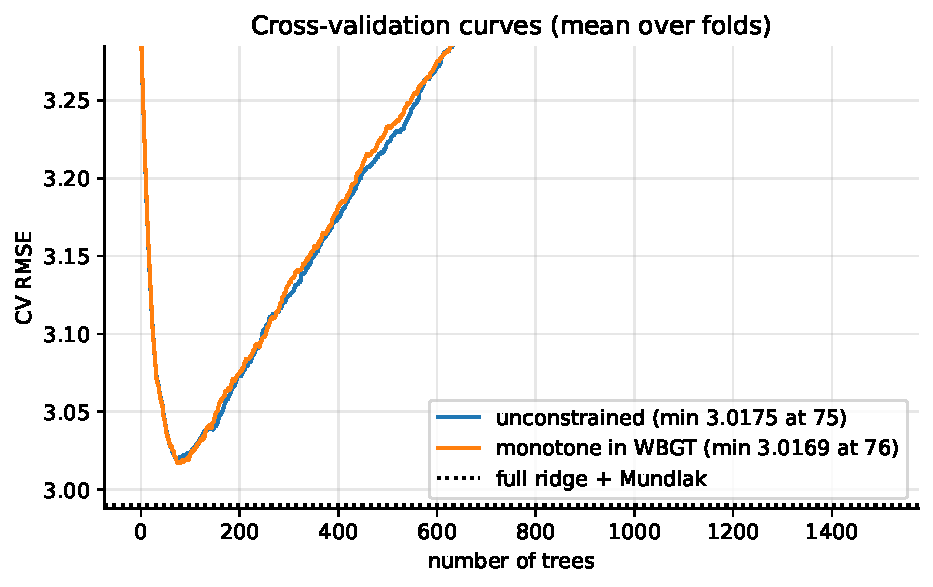
\includegraphics[width=0.62\textwidth]{gbm_cv}
\caption{Cross-validated RMSE by venue of gradient boosting as a function of the number of trees (mean over the five
folds), without constraint and with a monotonicity constraint in WBGT. The dotted line shows the RMSE of the full ridge
with the Mundlak term.}
\label{fig:gbm_cv}
\end{figure}

Both curves fall quickly during the first few dozen trees, reach their minimum around 75 trees, then rise steadily
(figure~\ref{fig:gbm_cv}): around 600 trees, the RMSE exceeds 3.25 and returns to the value obtained with a single
tree. With a learning rate of 0.03, 75 trees roughly correspond to the number needed to capture most of a simple
signal: the model stops as soon as it has learned the general regularities. Beyond that, each tree learns
particularities of the training venues, which do not transfer to the validation venues, and overfitting is fast.

Two lessons emerged. First, the monotonicity constraint costs nothing: the monotone model obtains an RMSE of 3.0169
with 76 trees, against 3.0175 with 75 trees without constraint. Imposing that heat never makes one run faster therefore
does not contradict the data, and this physiological knowledge can be injected without any loss of accuracy. Second,
boosting does no better than the linear models: with 3.017, it is on a par with the mixed model (3.013) and slightly
worse than ridge (2.990 to 2.996), differences below 0.03 whereas the standard error across folds is about 0.19. The
flexibility of trees brings nothing measurable. The signal that transfers from one venue to another is therefore
essentially smooth and close to additive (effects of age, level, form, duration), which linear models already
capture; the nonlinearities and interactions that trees could discover are either absent or too weak to be
distinguished from noise with some 300 races.

\subsection{Does the WBGT summarize the weather well? What does a flawed validation cost?}\label{sec:raw_weather}

Two experiments completed the study of boosting, with a number of trees chosen each time by the cross-validation
curve. The first compares four sets of meteorological variables, the other variables remaining the same: the WBGT with
wind and rain; the raw components (air temperature, humidity, wind, radiation, rain); the WBGT and its components; and
no meteorological variable at all. Two hypotheses were opposed. If the physical summary of the WBGT loses useful
information, for instance if humidity weighs more than formula \eqref{eq:wbgt} says, the raw components should predict
better; if on the contrary this summary is relevant, it should do at least as well with fewer variables, hence fewer
ways of overfitting.

The four sets lie within 0.01 of RMSE: 3.017 with the WBGT, 3.008 with the raw components as well as with the WBGT and
its components, and 3.014 without any meteorological variable. The model without weather therefore does as well as
the model with the WBGT, and the advantage of the raw components, twenty times smaller than the standard error across
folds, allows us to conclude neither that the WBGT loses information nor that it summarizes it well. On these data, the
sets of variables cannot be ranked by their predictive power.

This result does not contradict the effect of heat estimated in section~\ref{sec:which_estimator}, of about 2~points of
$y$ for 10~°C. It illustrates the difference between \emph{estimating an effect} and \emph{improving a prediction}. If
heat acts with a slope $b \approx 0.2$~point per degree and the WBGT varies with a standard deviation of about 4.4~°C,
the variance of $y$ due to heat is at most $b^2\,\Var(W) \approx 0.04 \times 19.5 \approx 0.8$. Relative to a residual
variance of about $3^2 = 9$, it would lower the RMSE by at most
$\sqrt{9} - \sqrt{9 - 0.8} \approx 0.8/(2 \times 3) \approx 0.13$, and only if the effect were perfectly known. The
actual gain is much smaller, for three reasons: a large part of the variation of the WBGT is already explained by the
event group and the time of day, hot track in the evening and cool marathon in the morning; the effect is
heterogeneous, strong in the marathon and zero in middle distance, where half of the hot races are found; and the
effect is estimated from some 300 races, few of them hot, so that estimation error absorbs part of the gain. A
potential gain of a few hundredths, drowned in a variability of 0.19 across folds, is invisible in cross-validation.
The quality of the tool will therefore be judged on the estimate of the effect and its uncertainty, not on the RMSE.

The second experiment compares, for the same model, cross-validation by venue and random five-fold cross-validation on
the rows. With random folds, the reported RMSE drops to 2.378, a performance overestimated by 21\%, and the number of
trees retained reaches 1,498, at the limit of the search: twenty times more than with folds by venue. With random
folds, each race has runners in training and in validation; the model can then memorize the specific effect of each
race (its date, venue, weather, field and dynamics) and give it back to the runners of the same race in validation. The
more trees it adds, the more finely it memorizes, and the better it ``predicts'': the validation curve no longer rises.
A model selected this way would be doubly misleading: its reported performance would be wrong, and its number of
trees, chosen to memorize, would make it heavily overfitted on a new venue, that is, exactly in the intended use of the
tool. Figure~\ref{fig:gbm_cv} shows what 1,500 trees cost on new venues: this is the empirical confirmation of the
information leakage described in section~\ref{sec:leakage}.

\section{A third family: neural networks}\label{sec:networks}

Until then we had two broad families of models: linear models, whose shape is fixed in advance, and trees, flexible
but stepwise. Neural networks form a third family, flexible like trees but producing smooth functions. Their smooth
shape could suit regular effects such as those of age, level or WBGT, which trees cut into steps. We present them
without assuming any prior knowledge.

\subsection{What is a neural network?}\label{sec:mlp}

Like all the models in this study, a neural network is a parameterized function $f_\theta$ that maps a vector of
variables $x$ to a prediction $\hat y = f_\theta(x)$, and whose parameters $\theta$ are learned by minimizing a loss on
examples. Its distinctive feature is that it belongs to a very rich family of functions: with enough parameters, it can
represent almost any relationship between $x$ and $y$, without the shape having to be specified. Neural networks are
behind recent progress in image recognition, machine translation and text generation, problems where data are massive
and unstructured and where nobody knows how to write down the shape of the relationship by hand. They also apply to
tabular data such as ours, but with less success.

The basic unit is the \emph{neuron}, which computes a linear combination of its inputs and then applies a nonlinear
function $\sigma$, called the \emph{activation}:
\[
h = \sigma\Big(\sum_{r=1}^{d} w_r\,x_r + b\Big) = \sigma(w^\top x + b),
\]
where the $w_r$ are the \emph{weights} and $b$ the \emph{bias}. In this section, $\sigma$ denotes an activation
function and not a standard deviation. A neuron has nothing mysterious about it: if $\sigma$ is the identity, it is
exactly a linear regression; if $\sigma$ is the sigmoid $z \mapsto 1/(1 + e^{-z})$, it is a logistic regression.

A network assembles neurons into \emph{layers}. A layer of $m$ neurons all receiving the same vector
$h \in \mathbb{R}^{d}$ reads $h' = \sigma(W h + b)$, with $W \in \mathbb{R}^{m \times d}$ and $b \in \mathbb{R}^{m}$,
each row of $W$ containing the weights of one neuron and $\sigma$ being applied componentwise. The \emph{multilayer
perceptron} chains $L$ layers, the output of one being the input of the next:
\begin{equation}\label{eq:mlp}
h_0 = x, \qquad h_k = \sigma(W_k\, h_{k-1} + b_k) \quad (k = 1, \dots, L), \qquad \hat y = w_{L+1}^\top h_L + b_{L+1} .
\end{equation}
The intermediate layers are called \emph{hidden}, since neither their inputs nor their outputs are observed. The
number of neurons in a layer is its \emph{width}, the number of layers the \emph{depth} of the network. A layer that
receives $d$ inputs and has $m$ neurons has $(d + 1)\,m$ parameters: their number grows quickly with width.

Without activation, a network would only be a disguised linear regression, since the composition of two affine
functions is affine: $W_2(W_1 x + b_1) + b_2 = (W_2 W_1)\,x + (W_2 b_1 + b_2)$. It is the activation that gives the
network its ability to represent nonlinear relationships. The sigmoid is smooth, but its derivative becomes very small
for large $\lvert z \rvert$, which slows down the training of deep networks. The ReLU activation, $\max(0, z)$, with
derivative 0 or 1, makes the network a piecewise affine function. The SiLU activation,
$z \mapsto z\,\mathrm{sig}(z)$ where $\mathrm{sig}$ is the sigmoid, is a smooth version of it, differentiable
everywhere, and it is the one we use. The ReLU activation gives a geometric intuition of the power of networks. Each
neuron of the first layer ``folds'' space along the hyperplane $w^\top x + b = 0$: it is 0 on one side and grows
linearly on the other. In one dimension, a sum $\sum_k c_k \max(0, x - s_k)$ is a broken line whose kinks are located at
$s_k$ and whose slope changes by $c_k$ at each kink; with enough kinks, a broken line approximates any continuous
curve. This is the idea of the following theorem.

\begin{theorem}[universal approximation; \citealp{cybenko1989, hornik1991, leshno1993}]
Let $\sigma$ be a continuous, non-polynomial activation function. For any continuous function $g$ defined on a compact
set $K \subset \mathbb{R}^d$ and any $\varepsilon > 0$, there exists a network with a single hidden layer of $N$
neurons,
\[
f_N(x) = \sum_{k=1}^{N} c_k\,\sigma(w_k^\top x + b_k),
\]
such that $\sup_{x \in K} \lvert g(x) - f_N(x) \rvert < \varepsilon$.
\end{theorem}

This theorem says that no continuous relationship is out of reach of a wide enough network. One must also know what it
does not say. It guarantees the existence of suitable weights, but does not say how to find them. The number of neurons
required can be enormous. It concerns the approximation of a function known over all of $K$, not learning from a
finite and noisy sample: a network able to represent anything is also able to represent the noise, that is, to
overfit. Finally, it says nothing about the behavior outside $K$: a network does not extrapolate reliably. The theorem
uses only one hidden layer, but depth is often more economical: some functions require an exponential number of
neurons with a single layer, and only a polynomial number with several layers \citep{telgarsky2016}.

\subsection{How a network learns}\label{sec:backprop}

We look for the parameters $\theta$ (all the matrices $W_k$ and all the biases) that minimize the empirical risk, here
the mean squared error $\hat{\mathcal R}(\theta) = \frac1n\sum_i (y_i - f_\theta(x_i))^2$. Unlike least squares, there is
no closed-form solution, and the function to minimize is not convex: it has many local minima and saddle points. We
proceed by gradient descent, starting from randomly drawn weights and moving step by step in the direction opposite to
the gradient, $\theta \leftarrow \theta - \eta\,\nabla_\theta \hat{\mathcal R}(\theta)$, where $\eta$ is the learning
rate. Too large, the steps make the optimization diverge; too small, it is very slow. Nothing guarantees reaching the
global minimum, but in practice the minima reached are often good. The result nevertheless depends on the initial
draw: two trainings with different random seeds give two different networks.

The gradient of the loss must be computed with respect to thousands of parameters. \emph{Backpropagation} does this
efficiently through the chain rule, applied layer by layer from the output to the input. Take a network with one
hidden layer, $z = W_1 x + b_1$, $h = \sigma(z)$, $\hat y = w_2^\top h + b_2$, and the loss of one observation
$\ell = \frac12(\hat y - y)^2$. Writing $\delta = \hat y - y$ for the prediction error and $\odot$ for the componentwise
product,
\[
\frac{\partial \ell}{\partial b_2} = \delta, \quad
\frac{\partial \ell}{\partial w_2} = \delta\,h, \quad
\frac{\partial \ell}{\partial z} = (\delta\,w_2) \odot \sigma'(z), \quad
\frac{\partial \ell}{\partial W_1} = \frac{\partial \ell}{\partial z}\,x^\top, \quad
\frac{\partial \ell}{\partial b_1} = \frac{\partial \ell}{\partial z} .
\]
The error $\delta$ is propagated backward through the weights $w_2$, then multiplied by the derivative of the
activation. The computation reuses the quantities of the forward pass and costs about as much as a prediction. One also
sees why the sigmoid hinders deep networks: its derivative, at most $1/4$, is multiplied once per layer, and the
gradient vanishes on its way back to the input.

Computing the gradient on all the data at each step would be costly. It is computed instead on a \emph{mini-batch} of
$n_{\text{batch}}$ observations drawn at random (128 or 256 here). The gradient of a mini-batch is an unbiased estimator
of the full gradient, noisier but much cheaper, and this noise even helps to escape poor local minima and saddle
points. An \emph{epoch} is a complete pass over the data, in mini-batches drawn in random order.

With a single learning rate, parameters with a large gradient move too fast, and those with a small gradient too
slowly. The Adam optimizer \citep{kingma2015} adapts the step of each parameter from two moving averages, that of the
gradient $g_t$ and that of its square:
\[
m_t = \beta_1 m_{t-1} + (1 - \beta_1)\,g_t, \qquad v_t = \beta_2 v_{t-1} + (1 - \beta_2)\,g_t^2, \qquad
\theta_t = \theta_{t-1} - \eta\,\frac{\hat m_t}{\sqrt{\hat v_t} + \epsilon},
\]
where $\hat m_t = m_t/(1 - \beta_1^t)$ and $\hat v_t = v_t/(1 - \beta_2^t)$ correct the bias due to initializing the
averages at 0, with $\beta_1 = 0.9$ and $\beta_2 = 0.999$ by default. The ratio $\hat m_t/\sqrt{\hat v_t}$ is of order 1
when the gradient is consistent and smaller when it is noisy: each parameter moves by about $\eta$ in a stable
direction, and cautiously in an uncertain one.

A network has many parameters: the one we use has about 11,000, for some 6,400 training performances. It can therefore,
in principle, memorize the training data, noise included, and must be regularized. We combined three regularizations.
Decoupled \emph{weight decay} \citep{loshchilov2019} shrinks the weights toward 0 at each step,
$\theta \leftarrow \theta - \eta\,\lambda\,\theta$, like a ridge regression; with Adam, this decoupled version differs
from a penalty $\lambda\lVert\theta\rVert^2$ added to the loss, whose gradient would be divided by $\sqrt{\hat v_t}$ and
therefore applied very unevenly across parameters. \emph{Dropout} \citep{srivastava2014} sets each neuron of a hidden
layer to zero with probability $p$, independently at each mini-batch, the neurons kept being multiplied by $1/(1 - p)$
so that the expected output does not change. The network can then rely neither on any particular neuron nor on a
fragile combination of neurons, and the effect is close to averaging a very large number of subnetworks; at prediction
time, all neurons are used. \emph{Early stopping}, finally, measures the validation loss at each epoch, keeps the
weights that minimized it, and stops training after a fixed number of epochs without improvement, the
\emph{patience}.

\subsection{The chosen network}\label{sec:architecture}

A network only handles numbers. For a categorical variable, we used \emph{embeddings} rather than one-hot encoding.
An embedding maps each category $m$ to a learned vector $e_m \in \mathbb{R}^{d_e}$, stored in a table $E$ with one row
per category. This is equivalent to multiplying the one-hot encoding of the category by $E$, that is,
$e_m = E^\top \mathbb 1_m$, a first linear layer without bias applied to the one-hot vector. The vectors are learned
together with the rest of the network, and two categories with similar effects end up with similar vectors. For a
variable with very many categories, a low-dimensional embedding summarizes thousands of one-hot columns into a dense
vector that shares information between similar categories. Our categorical variables have only 5 and 2 categories, so
the embedding brings little here; a category unknown at training time receives a reserved vector.

Our network is a multilayer perceptron whose input concatenates the standardized numerical variables and one embedding
per categorical variable:
\[
h_0 = \big(x^{\text{num}},\ e_{\text{group}},\ e_{\text{sex}}\big),\qquad
h_k = \mathrm{Dropout}\big(\mathrm{SiLU}(W_k\, h_{k-1} + b_k)\big),\qquad \hat y = w_{L+1}^\top h_L + b_{L+1} .
\]
The numerical variables are those of boosting (level, age, form, duration, altitude, time, WBGT, wind, rain and mean
WBGT of the course), plus the missing-value indicators for age and form, that is, 12 columns. The embedding of the event
group has dimension 4 and that of sex dimension 3, so that $h_0$ has 19 components. The target is also standardized on
the training set, then the predictions are brought back to the scale of $y$. For an architecture with two hidden layers
of 128 and 64 neurons, the network has $(19 + 1) \times 128 = 2{,}560$ parameters in the first layer,
$(128 + 1) \times 64 = 8{,}256$ in the second, $65$ in the output and $33$ in the two embedding tables, that is, 10,914
parameters.

Two networks trained with different seeds give different predictions: this is a source of variance specific to
non-convex optimization. We therefore average the predictions of $n_{\text{mod}}$ networks trained with different
seeds. If these predictors each have a variance $s^2$ and a pairwise correlation $\rho$, their mean has variance
\[
\Var\Big(\frac{1}{n_{\text{mod}}}\sum_{m=1}^{n_{\text{mod}}} f_m\Big) = \rho\,s^2 + \frac{1 - \rho}{n_{\text{mod}}}\,s^2 ,
\]
which decreases with $n_{\text{mod}}$ as long as the networks are not perfectly correlated, at no cost in bias.

\subsection{Overfitting, observed}\label{sec:overfitting}

To watch overfitting at work, we first trained a network of 128 and 64 neurons, without dropout or weight decay, with a
learning rate of $3\cdot10^{-3}$, on four folds of venues, monitoring the error on the fifth fold, made up of fourteen
new venues.

\begin{figure}[htbp]
\centering
\begin{minipage}[t]{0.49\textwidth}
\centering
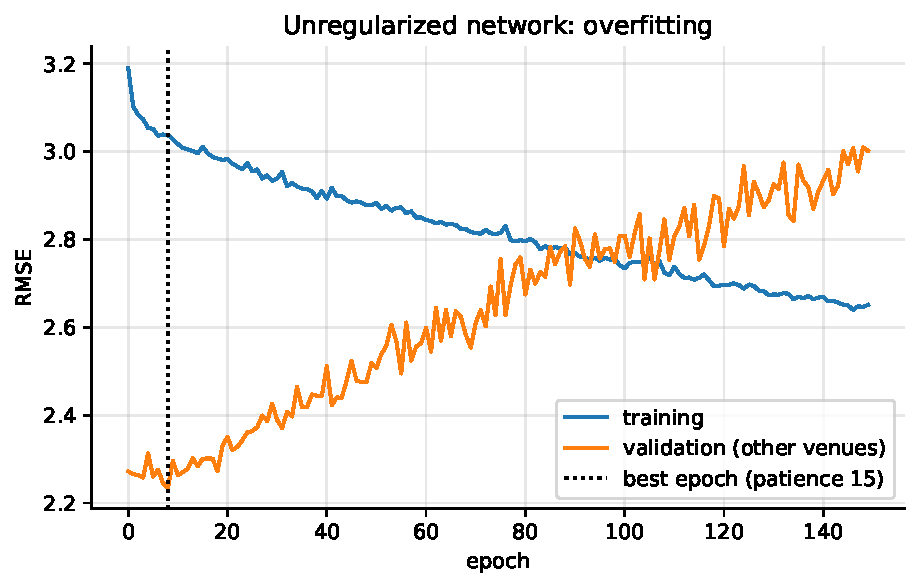
\includegraphics[width=\linewidth]{network_overfitting}
\end{minipage}\hfill
\begin{minipage}[t]{0.49\textwidth}
\centering
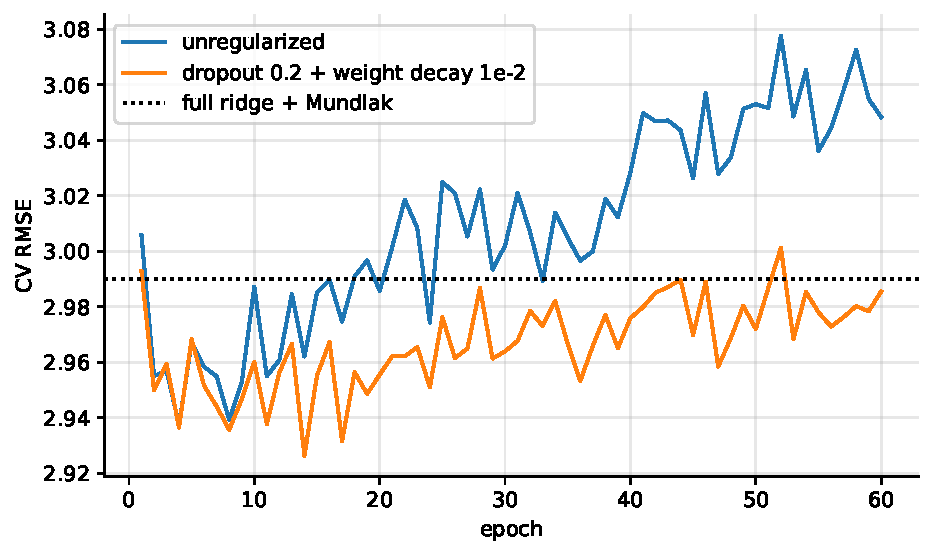
\includegraphics[width=\linewidth]{network_cv}
\end{minipage}
\caption{Left, training RMSE (four folds) and validation RMSE (fold~0, new venues) of an unregularized network over the
epochs; the dotted line marks the best validation epoch. Right, cross-validated RMSE (mean over the first three folds)
as a function of the number of epochs, without regularization and with dropout and weight decay; the dotted line shows
the RMSE of the full ridge over the five folds.}
\label{fig:network}
\end{figure}

Figure~\ref{fig:network} (left) shows the typical signature of overfitting. The training RMSE decreases without
interruption, from 3.19 at the first epoch to 2.65 at the 150th: the network fits the venues it sees better and better.
The validation RMSE, on the contrary, reaches its minimum as early as the 9th epoch, then rises almost linearly up to
3.00. From then on, each epoch improves the fit to the training venues at the expense of new venues: with about 11,000
parameters for 6,435 training performances, the network has ample room to memorize the noise and the particularities
of each venue. Early stopping, with a patience of 15 epochs, interrupts training at the 24th epoch and reloads the
weights of the 9th: the validation RMSE is then 2.235, against 3.002 at the end of training. Overfitting thus costs
0.77~point of RMSE, that is, $34$\%; without early stopping, the network even does clearly worse than the constant
model on this fold (2.647). That the validation error is at first lower than the training error is no paradox: fold~0
is the easiest of the five, its venues having less dispersed performances, and it is the evolution of the two curves
that matters. The value 2.235 is, moreover, optimistic, since the stopping epoch was chosen on this same fold, at the
lowest point of a noisy curve.

As for boosting, we therefore chose the number of epochs on the mean cross-validation curve. For lack of computing
time, this search covers the first three folds and at most 60 epochs, for two settings of a network of 128 and 64
neurons with a learning rate of $10^{-3}$: without regularization, and with dropout ($p = 0.2$) and weight decay
($\lambda = 10^{-2}$). The unregularized network reaches its minimum as early as the 4th epoch (RMSE of 2.937), then
rises above 3.05 from the 40th onward; the regularized network reaches its minimum at the 14th epoch (2.926), and its
curve stays between 2.93 and 3.00 over the 60 epochs (figure~\ref{fig:network}, right). Regularization hardly improves
the best value, but it makes the network much less sensitive to the number of epochs, which is valuable since this
number is chosen on a noisy curve.

The comparison with the other models calls for caution: the first three folds are easier than average, and the
network must be confronted with the other models on the same folds. The full ridge obtains 2.936 there without the
Mundlak term and 2.938 with it, the mixed model 2.977 and the constant model 3.281. The dotted line in the figure, which
represents ridge over the five folds, therefore flatters the network: on equal folds, the regularized network beats
ridge by only 0.01, and the unregularized network is on a par with it. These differences are much smaller than the
standard error across folds, all the more so as the curves oscillate by 0.02 to 0.03 from one epoch to the next: the
network does no better than a well-specified linear model. This is the expected result on tabular data of modest size
\citep{grinsztajn2022}, and it confirms the diagnosis drawn from boosting: the signal that transfers from one venue to
another is smooth and nearly additive, and a linear model already captures it.

One could, finally, have learned an embedding per race or per venue, the neural equivalent of a random intercept. It
would be useless here: all the races and venues evaluated are new, and their vector would never have been learned.
This is the \emph{cold-start} problem, the same one that cancels the BLUP of the mixed model in validation. The
personal best already plays the role of the athlete's individual effect, measured outside the race.

\section{Tuning, then comparing on unseen cities}\label{sec:comparison}

At this stage we had four families of models, built with reasonable initial settings. Two questions remained open:
can these models be improved by better tuning their hyperparameters? And, once each model is tuned, which one is the
best, and with what certainty? To answer the second, we used, for the first and only time, the test set set aside at
the beginning of the study.

\subsection{Random hyperparameter search}\label{sec:search}

A model has two kinds of settings. \emph{Parameters} are learned from the data by the algorithm itself: the
coefficients of a regression, the leaf values of a tree, the weights of a network. \emph{Hyperparameters} are set
before training and determine its form or intensity: learning rate, number of leaves, penalty, network architecture,
dropout rate. They mainly control the complexity of the model, that is, the trade-off between bias and variance, and
cannot be learned by minimizing the training error, which would always choose the most complex model. They are
therefore chosen by minimizing an estimate of the error on unseen data, here the cross-validated RMSE by venue.

Grid search tries all combinations of a fixed set of values for each hyperparameter. With $q$ hyperparameters and $k$
values each, $k^q$ evaluations are needed: 5 values for 7 hyperparameters already require $5^7 = 78{,}125$
cross-validations. Random search draws $N$ configurations at random in the search space. \citet{bergstra2012} showed
that for the same budget it explores better than a grid, for a simple reason: in practice, only a few hyperparameters
really matter, and one does not know in advance which ones. A grid of $N$ points tries only $N^{1/q}$ distinct values of
each hyperparameter, whereas a random draw tries $N$ of each. It also offers a simple guarantee. Call a configuration
``good'' if it lies among the best 5\% of the search space. Each draw has a probability $0.05$ of being one, so the
probability that at least one of the $N$ draws is good is $1 - 0.95^N$, which exceeds 95\% as soon as $N = 60$,
whatever the dimension of the space. With our budgets, 16 draws give a probability of 56\% of reaching the best 5\% of
configurations, and of 81\% of reaching the best 10\%.

Each hyperparameter is drawn from a distribution suited to its nature. For scale parameters, such as learning rates
and penalties, whose effect depends on the order of magnitude rather than on the absolute value, we use a
\emph{log-uniform} distribution: $U$ is drawn uniformly on $[\ln a, \ln b]$ and $x = e^U$. The density of $x$ is then
$1/\big(x \ln(b/a)\big)$ on $[a, b]$, and
\[
\mathbb{P}(x \leq c) = \frac{\ln(c/a)}{\ln(b/a)},
\]
so that each order of magnitude receives the same probability: on $[0.001, 0.1]$, $\mathbb{P}(x < 0.01) = 1/2$. With a
uniform distribution on $[0.01, 0.1]$, on the contrary, 56\% of the draws would fall above 0.05 and only 11\% below
0.02: small values, often the best ones, would almost never be tried. Proportions follow a uniform distribution,
counts a uniform distribution on the integers, and discrete options a uniform choice from a list.

For gradient boosting, 16 configurations were drawn, each evaluated on the five folds with the monotonicity constraint
and a number of trees chosen from the mean curve: learning rate log-uniform between 0.02 and 0.1, number of leaves
between 4 and 48, minimum number of performances per leaf between 20 and 250, penalty $\lambda$ log-uniform between 0.1
and 50, fractions of variables and of rows uniform between 0.5 and 1, and minimum gain $\kappa$ among 0, $0.001$ and
$0.01$. For the network, which is costlier, 5 configurations were evaluated on three folds: architecture among a single
layer of 32 neurons, two layers of 64 and 32 or of 128 and 64, and three layers of 64, 64 and 32; dropout uniform
between 0 and 0.3; learning rate log-uniform between $3\cdot10^{-4}$ and $3\cdot10^{-3}$; weight decay log-uniform
between $10^{-5}$ and $3\cdot10^{-2}$; embedding dimension among 2, 4 and 8; mini-batches of 128 or 256.

Choosing the best of $N$ configurations on the cross-validated RMSE introduces a \emph{selection bias}. Each estimated
RMSE contains a share of noise, and the configuration retained is the one whose estimate is the lowest, which favors
those whose noise was favorable:
\[
\E\Big[\min_{k \leq N} \widehat{\mathrm{RMSE}}_k\Big] \leq \min_{k \leq N} \E\big[\widehat{\mathrm{RMSE}}_k\big] .
\]
This is the same inequality as for choosing the number of trees, at the scale of the whole configuration. In the
simplest case, where $N$ configurations would have the same true error and independent estimation errors with the same
standard deviation $s$, the most favorable one would on average be $1.8\,s$ below the true error for $N = 16$: this is
the expectation of the maximum of 16 standard normal variables, which grows like $\sqrt{2\ln N}$. In practice the
effect is smaller, because all configurations are evaluated on the same folds and their estimation errors are highly
correlated. The cross-validation score of the winner nevertheless remains optimistic, and it is the role of the test
set to correct it.

For gradient boosting, the explored surface turned out to be a plateau. The six best configurations lie within 0.005
of RMSE although their hyperparameters are very different, with learning rates from 0.02 to 0.06 and from 31 to 159
trees: the precise value of the hyperparameters matters very little, which is exactly the situation described by
\citet{bergstra2012}. The best configuration drawn (learning rate of 0.020, 21 leaves, at least 218 performances per
leaf, $\lambda = 0.12$, 86\% of the variables and 59\% of the rows per tree, 159 trees) obtains 3.0278, slightly worse
than the initial setting (3.0169). That setting does belong to the search space, but none of the sixteen draws fell
into such a good region, which is not surprising with a one-in-two chance of reaching the best 5\% of configurations;
the difference, 0.011, is in any case of no practical consequence, and we kept the configuration drawn. A clear trend
emerges: five of the six best configurations require at least 129 performances per leaf. Such a populated leaf can
isolate neither a race nor even a small venue: these trees are strongly regularized, which confirms that the
transferable signal is smooth. The same setting without the monotonicity constraint finally obtains 3.0335 with 130
trees: the constraint still costs nothing.

For the network, the five configurations lie within 0.018, with architectures as different as a single layer of 32
neurons and three layers of 64, 64 and 32. The least regularized configuration (dropout of 0.08, no weight decay) comes
last, and the best one, with an RMSE of 2.922 on three folds, has the strongest dropout: three layers of 64, 64 and 32
neurons, dropout of 0.27, learning rate of $1.2\cdot10^{-3}$, weight decay of $3.4\cdot10^{-3}$, embeddings of
dimension 4, mini-batches of 256 and 14 epochs. Learning rate and number of epochs go hand in hand: with a rate of $3$
to $4\cdot10^{-4}$, 24 to 58 epochs are needed to reach the minimum. On the same folds, ridge obtained 2.936 to 2.938:
the lead of the best network, 0.015, is much smaller than the standard error, and partly the effect of selection bias.
The final network averages five networks with this setting.

\subsection{The final evaluation}\label{sec:test}

All models were retrained on the 79 training venues together, with the hyperparameters chosen by cross-validation,
then evaluated once on the 21 test venues (2,355 performances, 102 races). This evaluation is fair because no choice
was made by looking at the test set. Nine models are compared: the constant model; the means by event and sex; least
squares on the WBGT alone; the best full ridge, with the Mundlak term; the race random-intercept model retained by the
one-standard-error rule; the tuned gradient boosting, with and without the monotonicity constraint; the ensemble of
five networks; and an \emph{ensemble} that averages the predictions of the mixed model, the monotone boosting and the
networks.

The idea behind this last ensemble rests on a convexity inequality. If $e_1, e_2, e_3$ are the errors of three models
on a performance, the error of their mean is the mean of the errors, and
$\big(\frac{e_1 + e_2 + e_3}{3}\big)^2 \leq \frac{e_1^2 + e_2^2 + e_3^2}{3}$; averaging over performances,
\[
\mathrm{MSE}(\text{ensemble}) \leq \frac{\mathrm{MSE}_1 + \mathrm{MSE}_2 + \mathrm{MSE}_3}{3} .
\]
The ensemble always does at least as well as the average of its members, and all the better as their errors are weakly
correlated. Models from different families are expected to make different kinds of mistakes.

With only 21 venues, the test RMSE is itself uncertain: another draw of test venues would give another value. To
quantify this uncertainty, we use the \emph{bootstrap} \citep{efron1979}. One would like to know the distribution of a
statistic over samples drawn from the population, but only one sample is available. The idea of the bootstrap is to
replace the population by the sample itself: new samples of the same size are drawn with replacement from the sample,
and the statistic is recomputed on each. The dispersion of the $B$ values obtained mimics the one that would be observed
on genuinely new samples, and the 95\% percentile confidence interval is formed by the $0.025$ and $0.975$ quantiles of
the $B$ replicates. We take $B = 2{,}000$: a $0.025$ quantile is then estimated from the 50 most extreme replicates,
which makes it stable.

The bootstrap, however, assumes that the resampled units are independent. Since prediction errors within a race, and
even within a venue, are correlated, resampling performances one by one would underestimate the uncertainty, exactly
like naive standard errors. We therefore resample \emph{venues}: 21 venues are drawn with replacement among the 21 test
venues, all their performances are pooled, and the RMSE is recomputed. The resampling unit is thus the same as the
grouping unit of the validation. To compare two models $A$ and $B$, finally, one does not compare their two intervals:
one computes the difference of their RMSEs on each of the same replicates, then the interval of this difference. This
is much more precise, since
\[
\Var(R_A - R_B) = \Var(R_A) + \Var(R_B) - 2\,\Cov(R_A, R_B),
\]
and the covariance is strongly positive: a venue that is hard to predict increases the error of all models at once. If
the interval of the difference excludes 0, the difference is significant at the 5\% level. The constant model serves as
the reference (table~\ref{tab:test}).

\begin{table}[htbp]
\centering
\small
\caption{Final evaluation on the 21 test venues (2,355 performances). 95\% confidence intervals from a venue bootstrap
($B = 2{,}000$); the difference from the constant model is computed replicate by replicate.}
\label{tab:test}
\begin{tabular}{@{}lcccccc@{}}
\toprule
Model & RMSE & 95\% CI & Diff.\ from constant & 95\% CI of the diff. & $R^2$ & MAE \\
\midrule
ensemble (mixed, boosting, networks) & 2.877 & [2.50, 3.27] & $-0.314$ & [$-0.52$, $-0.17$] & 0.172 & 2.136 \\
mixed (race intercept) & 2.896 & [2.52, 3.29] & $-0.295$ & [$-0.51$, $-0.14$] & 0.162 & 2.149 \\
monotone boosting & 2.898 & [2.52, 3.29] & $-0.294$ & [$-0.49$, $-0.16$] & 0.161 & 2.151 \\
networks (ensemble of 5) & 2.902 & [2.51, 3.30] & $-0.289$ & [$-0.50$, $-0.14$] & 0.158 & 2.160 \\
free boosting & 2.902 & [2.52, 3.30] & $-0.289$ & [$-0.47$, $-0.16$] & 0.158 & 2.155 \\
full ridge with Mundlak & 2.944 & [2.49, 3.41] & $-0.247$ & [$-0.53$, $-0.11$] & 0.133 & 2.214 \\
least squares on the WBGT & 3.142 & [2.73, 3.61] & $-0.050$ & [$-0.14$, $+0.05$] & 0.013 & 2.383 \\
constant & 3.191 & [2.70, 3.71] & 0 & -- & $-0.018$ & 2.422 \\
means by event and sex & 3.305 & [2.78, 3.86] & $+0.113$ & [$-0.03$, $+0.22$] & $-0.092$ & 2.501 \\
\bottomrule
\end{tabular}
\end{table}

The models that use the athletes' profile clearly beat the constant model: they reduce the RMSE by 0.25 to
0.31~point, and all the intervals of these differences exclude 0. Their test $R^2$ ranges from 0.13 to 0.17: about one
sixth of the variance of performances is predictable on a never-seen venue. The rest, form on the day, tactics, age of
the personal best, is not. The naive models, for their part, do no better than the constant. The WBGT alone gains
0.05~point, with an interval that contains 0: heat, taken alone, does not predict performance. The means by event and
sex even do worse than the constant, as in cross-validation.

The order among the best models is not established. Five models lie within 0.025 of RMSE, and the mixed model, the two
boostings and the networks within 0.006; their differences from the constant model have intervals that overlap almost
entirely. The model families are equivalent in prediction. One reversal is nevertheless worth noting: ridge, slightly
better in cross-validation, is the worst of the models with controls on the test set, whereas the mixed model,
slightly worse in cross-validation, is among the best. The retained ridge is a degree-3 polynomial with interactions,
chosen by the smallest RMSE, whereas the mixed model has degree~1, chosen by the one-standard-error rule. This reversal
is in line with our concern: a more complex model, chosen on non-significant differences, transfers less well to new
venues. The difference between the two, 0.048, nevertheless remains too small to prove it.

The ensemble is the best model, but gains little. In line with the convexity inequality, its squared error is lower
than the average of those of its three members:
\[
2.877^2 = 8.28 \;<\; \tfrac13\big(2.896^2 + 2.898^2 + 2.902^2\big) = 8.40 .
\]
The gain is only 1.5\%, however, because the three models almost always err in the same direction on the same
performances: the correlation between their errors is 0.97 to 0.99. What they cannot predict, form on the day, none of
them can. Likewise, the five networks of the ensemble have, taken separately, test RMSEs of 2.89 to 2.92: averaging the
seeds does not make the network better than its best member, but avoids depending on an unlucky seed.

The intervals are wide: that of the RMSE of the ensemble ranges from 2.50 to 3.27. There are only 21 venues, and some
weigh very heavily: Portland alone accounts for 686 performances (29\% of the test set) and Valencia for 415 (18\%).
Depending on whether these venues are drawn zero, one or two times in a replicate, the RMSE changes a lot. The interval
of the difference from the constant model is twice as narrow, because the difference removes the common share of
difficulty. Note finally that the test RMSEs are lower than the cross-validation ones (2.88 to 2.94 against 2.99 to 3.03
for the models with controls, 3.19 against 3.30 for the constant): the test venues are slightly less heterogeneous than
the average fold, and it is the differences between models that should be compared, not the absolute levels.

This assessment shaped the rest of the work. In prediction, the four model families are on a par: a degree-1 linear
mixed model does as well as a tuned boosting or an ensemble of networks. The choice of the tool's model therefore could
not be made on predictive accuracy. It had to be made on the quality of the estimate of the effect of heat:
readability of the degradation curve, absence of bias and honest uncertainty.

\section{What the models learned about heat}\label{sec:interpretation}

The tool does not need the best prediction of a race time, but a reliable estimate of the \emph{effect} of weather
conditions. Since the models are on a par in prediction, we opened them up to see what they had learned. This step
brought out the most important result of the study: models of identical accuracy tell different stories about heat.

\subsection{Attributing a prediction to the variables: Shapley values}\label{sec:shap}

For a linear model, the contribution of a variable to a prediction can be read directly: it is the product of its
coefficient and its value. For a boosting of 159 trees, there is nothing of the kind, since the same variable is
involved in hundreds of splits, in interaction with the others. Cooperative game theory, however, answers an analogous
question: how to share fairly the gain of a coalition among its players, when each player's contribution depends on
the others \citep{shapley1953}? The ``players'' are here the $p$ variables, and the ``gain'' is the prediction. For a
performance $x$, let $v(S) = \E\big[f(X) \mid X_S = x_S\big]$ be the expected prediction when only the variables in
the set $S$ are known, the others being replaced by their distribution in the data; $v(\varnothing) = \E[f(X)]$ is the
mean prediction and $v(\{1, \dots, p\}) = f(x)$ the full prediction. The \emph{Shapley value} of variable $j$ is
\begin{equation}\label{eq:shapley}
\phi_j(x) = \sum_{S \subseteq \{1, \dots, p\} \setminus \{j\}} \frac{|S|!\,(p - |S| - 1)!}{p!}\,
\big[v(S \cup \{j\}) - v(S)\big].
\end{equation}
The difference $v(S \cup \{j\}) - v(S)$ is the marginal contribution of $j$ when it joins the set $S$. The coefficient
$|S|!\,(p - |S| - 1)!/p!$ is the probability that, in an order of arrival of the variables drawn at random among the
$p!$ possible orders, the variables that arrived before $j$ are exactly those of $S$. The Shapley value is thus the
marginal contribution of $j$ averaged over all orders of arrival: no order is privileged. With two variables, for
example, $\phi_1(x) = \frac12\big[v(\{1\}) - v(\varnothing)\big] + \frac12\big[v(\{1, 2\}) - v(\{2\})\big]$ is the mean
of the contribution of variable~1 when it arrives first and when it arrives second. Shapley values are the unique
allocation satisfying four properties: efficiency, $f(x) = \phi_0 + \sum_{j} \phi_j(x)$ with $\phi_0 = \E[f(X)]$, which
decomposes the prediction exactly; symmetry, which gives the same contribution to two variables playing the same role;
a zero contribution for a variable that never changes the prediction; and additivity, which makes the contributions of
a sum of models, such as a boosting, add up. The formula requires $2^{p-1}$ terms per variable, but for trees the
TreeSHAP algorithm computes the exact values in polynomial time \citep{lundberg2017, lundberg2020}. We applied it to
the monotone boosting, on the test venues.

\begin{figure}[htbp]
\centering
\begin{minipage}[c]{0.53\textwidth}
\centering
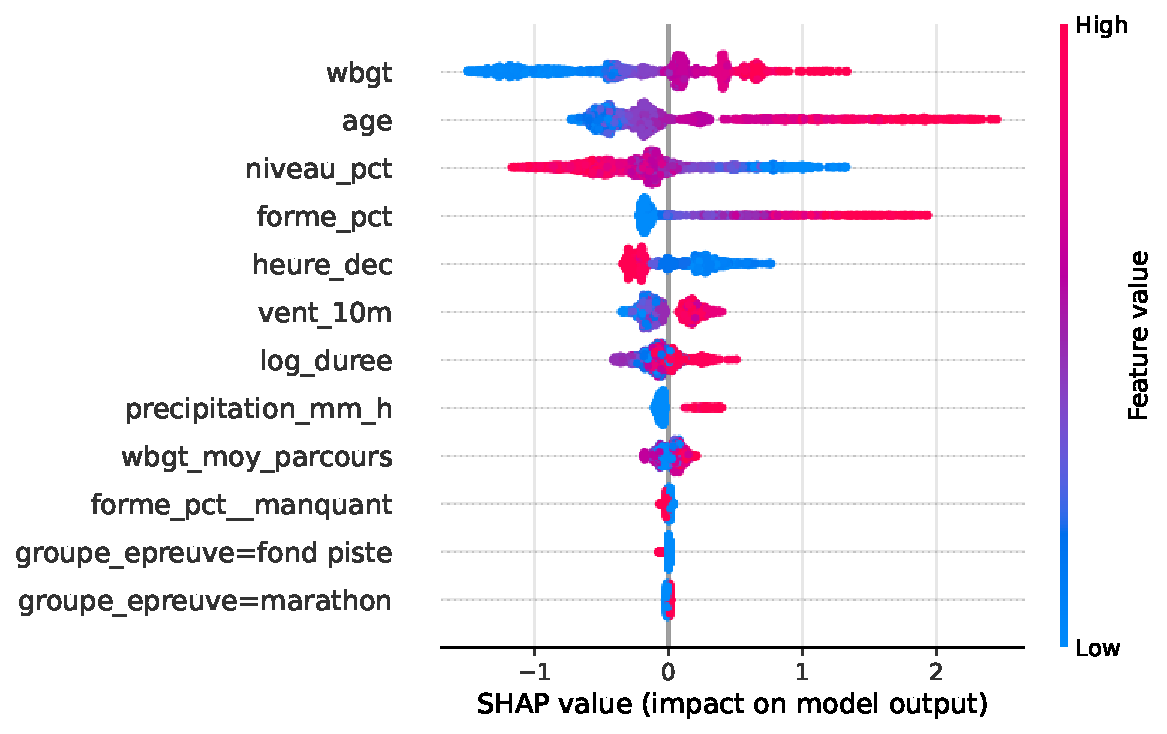
\includegraphics[width=\linewidth]{shap_summary}
\end{minipage}\hfill
\begin{minipage}[c]{0.45\textwidth}
\centering
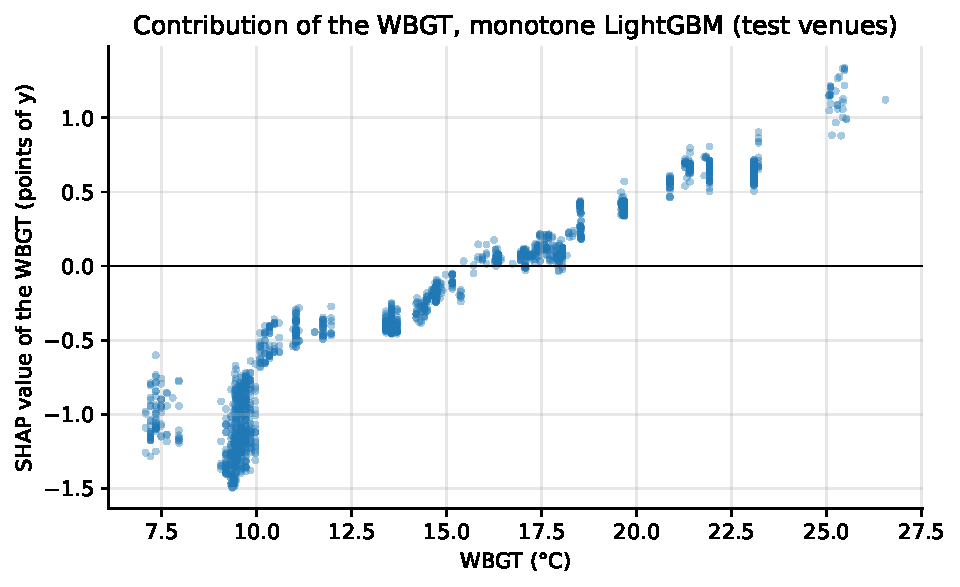
\includegraphics[width=\linewidth]{shap_wbgt}
\end{minipage}
\caption{Shapley values of the monotone boosting on the test venues. Left, one row per variable and one point per
performance, colored by the value of the variable (\texttt{niveau\_pct}: level; \texttt{heure\_dec}: start time;
\texttt{log\_duree}: logarithm of the expected duration; \texttt{wbgt\_moy\_parcours}: mean WBGT of the course). Right,
contribution of the WBGT as a function of its value.}
\label{fig:shap}
\end{figure}

The global importance of a variable is the mean of $|\phi_j|$ over the performances, in points of $y$. The WBGT is the
most important variable of the model, with a mean contribution of 0.55~point, ahead of age (0.50), level (0.39), form
(0.29), start time (0.24), wind (0.16), expected duration (0.13), rain (0.07) and the mean WBGT of the course (0.07);
the event-group indicators receive almost zero contributions (figure~\ref{fig:shap}). The contribution of the WBGT
increases stepwise, from $-1.4$~points around 9.5~°C to $+1.2$~points around 25~°C. The points form vertical bands,
each band corresponding to a race whose runners all share the same WBGT; and the contributions are measured relative to
the mean prediction $\phi_0$, not relative to the reference WBGT. The direction of the effects is as expected: a high
WBGT, an older age, a form far from the personal best, strong wind, rain and a long duration slow runners down relative
to their best. A late start time is associated with performances closer to the personal best, since evening track
meetings offer fast tracks and pacemakers. An athlete slower than the median of their event also runs closer to their
best; several explanations are possible, such as a less exceptional personal best or the selection by the truncation
margin, and the model cannot separate them.

This result seems to contradict that of section~\ref{sec:raw_weather}, where removing all meteorological variables did
not worsen the RMSE. The two are compatible. The WBGT is strongly linked to the event group and to the time of day: when
it is present, part of the information it carries could also be carried by these variables, and the Shapley value
gives it the credit; when it is absent, time, duration and group take over. A high Shapley value means neither that a
variable is indispensable to the prediction nor that it has a causal effect: it describes the model, not the world. To
measure the effect of heat for a given athlete profile, another tool was needed.

\subsection{Partial dependence and the degradation curve}\label{sec:pd}

The \emph{partial dependence} of a model $f$ on a variable $v$ \citep{friedman2001} is the function
\[
\mathrm{PD}_v(\xi) = \frac1n\sum_{i=1}^n f\big(x_i \text{ with } x_{i,v} = \xi\big):
\]
for each value $\xi$, one imposes $x_{i,v} = \xi$ on all performances, the other variables keeping their observed
values, and averages the predictions. It answers the question: ``what would the model predict, on average over our
athletes and races, if variable $v$ were equal to $\xi$ for everyone?'' Unlike the mean of $y$ by WBGT class, which
compares different races, partial dependence compares the same performances under two values of the variable: the
composition of events, age and level are identical from one value to another, which neutralizes Simpson's paradox
within the model. Before averaging, each performance $i$ has its own curve
$\xi \mapsto f(x_i \text{ with } x_{i,v} = \xi)$, called an ICE curve \citep{goldstein2015}. Their dispersion is
informative about interactions: if all ICE curves are parallel, the effect of $v$ is the same for all performances; if
they diverge, it depends on the other variables.

The degradation curve is the partial dependence on the WBGT, centered on the reference:
\begin{equation}\label{eq:degradation_curve}
\Delta(W) = \mathrm{PD}_{\WBGT}(W) - \mathrm{PD}_{\WBGT}(W_{\text{ref}}),
\end{equation}
in points of $y$, that is, approximately in percent of speed. This is exactly the quantity the tool needs
\eqref{eq:degradation}: the mean degradation of performance when the WBGT goes from 15~°C to $W$, for an unchanged
athlete profile. For a degree-1 linear model without interaction, all ICE curves are parallel straight lines and
$\Delta(W) = \beta_W\,(W - W_{\text{ref}})$. If the model contains the Mundlak term $\bar W_g$, it is left unchanged:
we measure the effect of a change in WBGT on a given course, that is, the within-course effect. Two precautions are in
order when reading these curves. At the ends of the grid, few performances have been observed, and the curve rests on
very few races there or simply extends the shape of the model; our figures shade the extreme 2.5\% of the data on each
side. And imposing a WBGT of 27~°C on a race run early on a winter morning creates combinations that do not exist in
the data: partial dependence remains a description of the model, whose causal interpretation relies on the controls
included and on the absence of omitted confounders.

\begin{figure}[htbp]
\centering
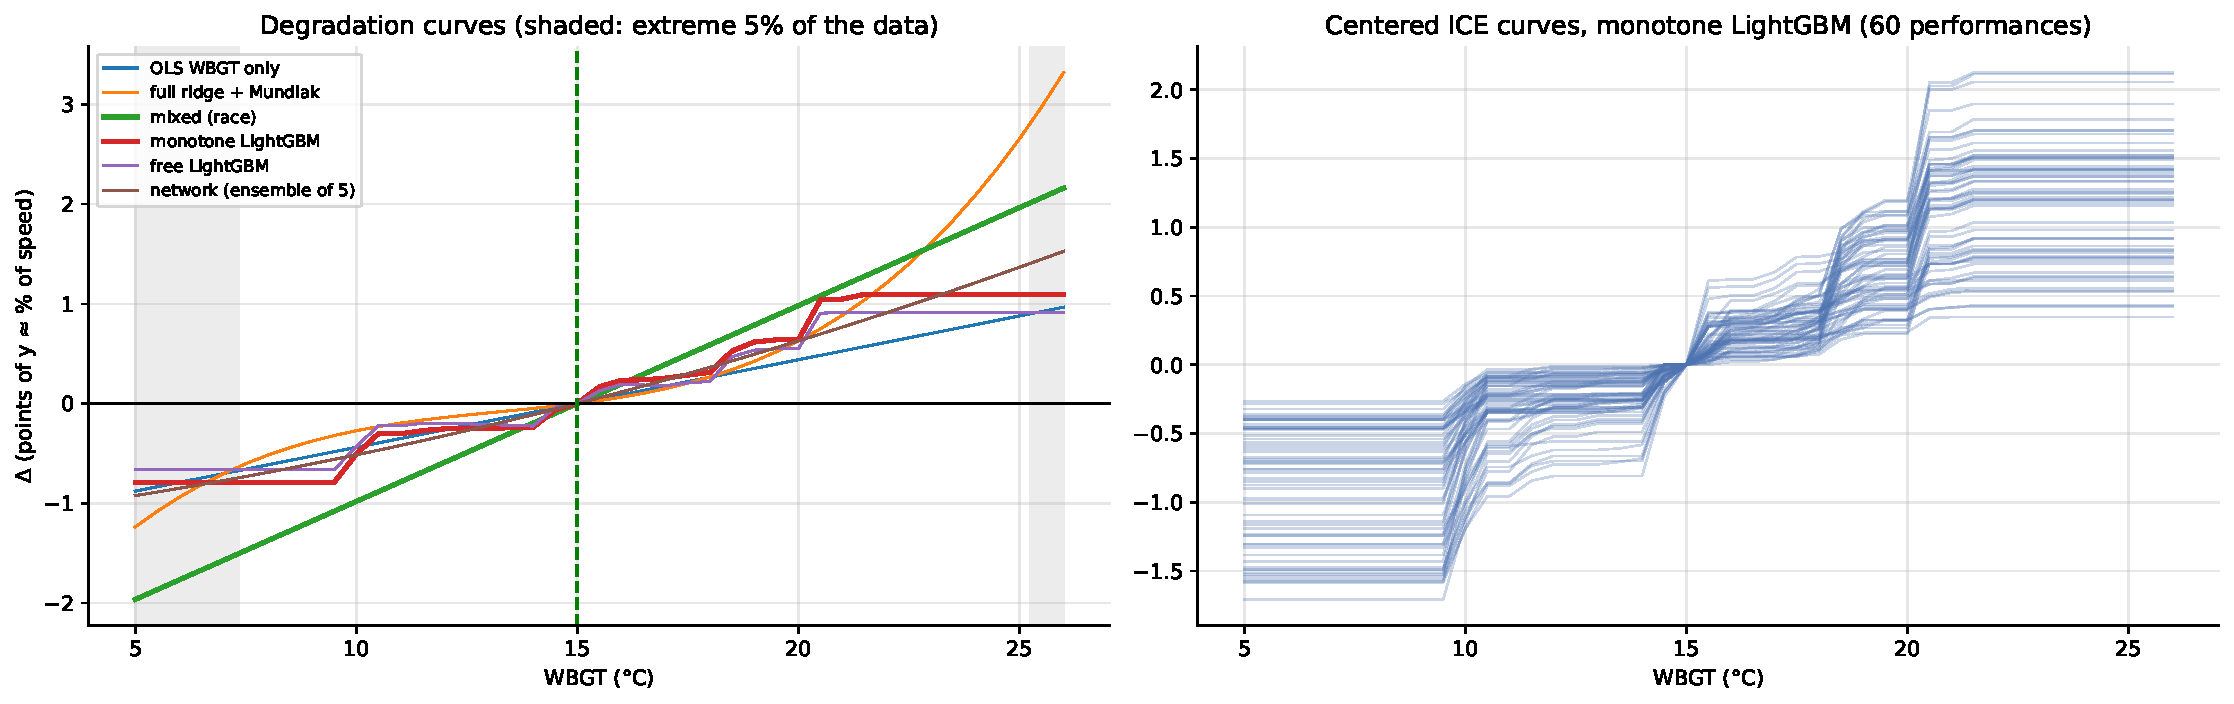
\includegraphics[width=\textwidth]{model_curves}
\caption{Left, degradation curves $\Delta(W)$ of six models, averaged over the training performances, all events
together; the shaded areas cover the extreme 2.5\% of the data on each side. Right, centered ICE curves of the
monotone boosting for 60 performances drawn at random.}
\label{fig:model_curves}
\end{figure}

The degradation curves of the six models all have the same direction: hotter, slower (figure~\ref{fig:model_curves}).
But their amplitude and shape differ markedly beyond 20~°C. At 25~°C, the degradation is about $+0.9$~point for least
squares on the WBGT alone, which control no confounder; $+1.1$ for the two boostings, whose stepwise curve becomes
constant beyond about 21~°C; $+1.4$ for the ensemble of networks, whose curve is smooth and almost linear; $+1.9$ for
the mixed model, whose curve is a straight line; and $+2.6$ for the full ridge, whose degree-3 polynomial is convex. The
trees level off: beyond the last threshold learned on the WBGT, for lack of enough hot races, they predict the same
whatever the WBGT. The degree-3 polynomial, on the contrary, shoots up: its curvature is carried by the few hottest
races, and exceeds 3~points in the shaded area, where data are missing. On the cool side, all models predict a faster
performance than at 15~°C, with a gap between them that widens below 7.5~°C, from $-0.8$ to $-1.9$~points at 5~°C. The
ICE curves of the boosting, finally, are far from parallel: at 25~°C, the degradation ranges from about $+0.4$ to
$+2.1$~points depending on the performance. The effect of heat therefore depends on the other variables, event,
duration or time of day, which justifies estimating one effect per event group. The steps, located around 10, 14.5,
18.5 and 20.5~°C, are the split thresholds of the trees, shared by all performances.

We were thus faced with an awkward finding: five models of indistinguishable accuracy give, for a 10~°C increase,
effects ranging from one to three. Predictive accuracy does not allow us to choose between them; it is the shape they
impose, or do not impose, on the curve that makes the difference. The tool's model had to be chosen on other criteria,
and the uncertainty of its curve had to be measured.

\subsection{Uncertainty on the curve: the venue bootstrap}\label{sec:curve_bootstrap}

For the tool, the models are now retrained on all venues, training and test together. The test set has already served
for the evaluation, and there is no longer any choice to be made by looking at it: using it to estimate the effect
creates no leakage, and 21 more venues improve precision.

The uncertainty on $\Delta(W)$ comes mainly from the small number of venues and races: each race brings only one
weather situation, and hot races are rare. We estimate it with a venue bootstrap, but this time retraining the model on
each replicate. We draw with replacement as many venues as there are in the data, pool all their performances and
retrain the model on this sample, then compute the degradation curve of the retrained model on a fixed reference
population; after $B$ repetitions, we take, point by point on the grid, the $0.025$ and $0.975$ quantiles of the $B$
curves. This yields a \emph{pointwise} 95\% confidence band: for each WBGT value, the interval contains the true value
of the curve with a probability of about 95\%. It is not a \emph{simultaneous} band, and the probability that the whole
curve stays within the band is lower. This bootstrap measures the uncertainty due to the sample of venues, including
the variability of the estimates of all coefficients, but not that due to a wrong choice of model shape.

Two precautions are essential. The curve is always computed on the same reference population, and not on the bootstrap
sample, whose composition changes at each replicate: otherwise, the measured variability would mix that of the model
with that of the population over which we average. And each copy of a venue drawn several times must become a distinct
venue, with its own races. Without this precaution, the races of a venue drawn twice would become races of double size,
made of pairs of identical rows: a mixed model would see an artificially small within-race variance and could estimate
$\gamma \to \infty$, with aberrant effects. In the logic of the bootstrap, each draw moreover represents a new venue of
the population.

\subsection{The model chosen for the tool}\label{sec:tool_model}

For the tool, what matters is the effect of the conditions: estimated with as little bias as possible, with an honest
uncertainty, readable by event, and without fanciful extrapolation. We retained a linear model with a random race
intercept, whose terms are chosen a priori from physiology and the literature. For performance $j$ of race $g$,
\begin{multline}\label{eq:tool_model}
y_{gj} = u_g + \sum_e \mathbb 1_e\,P_e(W_{gj}) + \beta_{W,\text{lev}}\,\frac{\text{level}_{gj}}{10}\,(W_{gj} - W_{\text{ref}})
+ \sum_e \mathbb 1_e\,\beta_{\text{alt},e}\,\text{alt}_g \\
+ \beta_{\text{wind}}\,\text{wind}_{gj} + \beta_{\text{rain}}\,\text{rain}_{gj} + x_{gj}^\top\beta + \varepsilon_{gj},
\end{multline}
with $u_g \sim \mathcal N(0, \tau^2)$ and $\varepsilon_{gj} \sim \mathcal N(0, \sigma^2)$. The term $P_e$ is a
polynomial in the WBGT specific to each event group $e$, and $\mathbb 1_e$ equals 1 for performances of group $e$: the
effect of heat can thus grow with the duration of the effort. The polynomials are written in the basis $\psi(W)$, which
vanishes at $W_{\text{ref}}$, and their degree is chosen by cross-validation by venue. The term $\beta_{W,\text{lev}}$
multiplies the WBGT difference from the reference by the athlete's level, in tens of points: it tests the finding of
\citet{ely2007} that slower runners are more affected by heat. Altitude above 500~m, $\text{alt}_g$, has a slope
specific to each group; since the tracks in our data are all below 300~m, its coefficient is zero for the two track
groups, and the tool will refuse any altitude higher than the one observed for the group. The controls $x_{gj}$ include
age, form, time of day, expected duration, level, sex and event group. We did not include a Mundlak term: with an effect
specific to each group, a course mean per group would be needed, and we saw that the within-course effect is not weaker
than the effect estimated without distinction.

This choice rules out the other two serious candidates. The curve of the monotone boosting is constrained to increase:
if the true effect is zero, it is biased upward, and its bootstrap interval cannot contain negative values above the
reference; it is also stepwise, and levels off beyond the last thresholds learned. The curve of the network is smooth,
but it does not decompose by event, and its uncertainty would require retraining ensembles of networks hundreds of
times. The linear mixed model gives a smooth curve, specific to each event, each term of which has an interpretation and
a confidence interval.

Cross-validation by venue gives an RMSE of 3.024 for a linear effect of the WBGT in each group, 3.028 with degree~2 and
3.042 with degree~3: degree~1 is retained, since the data do not allow a curvature specific to each group to be
estimated, and the one-standard-error rule would have made the same choice.

\paragraph{An unexpected difficulty: the REML likelihood is bimodal.} While estimating this model, we found that the
profile restricted log-likelihood $\ell_R(\gamma)$ does not always have a single maximum. Besides the interior maximum,
it can rise again toward the boundary $\gamma \to \infty$, which corresponds to race fixed effects
(figure~\ref{fig:reml_profile}). The main cause is heteroscedasticity: the standard deviation of $y$ within a race is
about 1.9~points in middle distance and 3.6 in the marathon, whereas the model assumes a common $\sigma^2$. By treating
each race as a fixed effect, the model absorbs part of this heterogeneity into the race means, which the likelihood may
reward. On the full sample, the interior maximum is reached at $\ln\hat\gamma = -2.12$, that is, $\hat\gamma = 0.120$,
with $\hat\tau^2 = 0.945$ and $\hat\sigma^2 = 7.873$: the race explains 11\% of the residual variance. The likelihood
then decreases to about $-16{,}585$ around $\ln\gamma \approx 2.8$, then rises again to $-16{,}396$ at the boundary
$\ln\gamma = 6$; the interior maximum ($-16{,}192$) wins by more than 200 log-likelihood units. But in a bootstrap
replicate, the boundary could win: race-level variables (WBGT, altitude, event group) would then be identified only by
the tiny variation that remains within races, and their effects would become aberrant.

\begin{figure}[htbp]
\centering
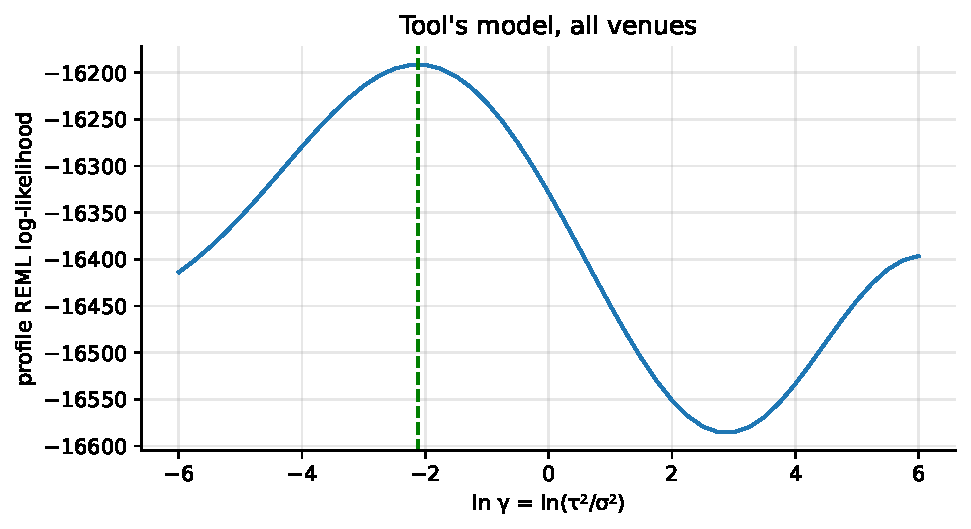
\includegraphics[width=0.6\textwidth]{reml_profile}
\caption{Profile restricted log-likelihood of the tool's model, estimated on all venues, as a function of $\ln\gamma$.
The dotted line marks the interior maximum, at $\ln\hat\gamma = -2.12$; the rise toward the right boundary corresponds
to race fixed effects.}
\label{fig:reml_profile}
\end{figure}

We solved this difficulty by fixing $\gamma$ at its value estimated on the full sample, $\hat\gamma$, in all replicates.
Each replicate then computes a generalized least squares estimator with a fixed \emph{working} covariance matrix
$V = V(\hat\gamma)$, $\hat\beta = (X^\top V^{-1} X)^{-1} X^\top V^{-1} y$. This estimator remains unbiased even if $V$ is
not the true covariance: since $\E[y] = X\beta$,
\[
\E[\hat\beta] = (X^\top V^{-1} X)^{-1} X^\top V^{-1} X\beta = \beta,
\]
whatever the matrix $V$ used. An imperfect matrix only costs precision. Its variance, however, is no longer the one given
by the model formula: if the true covariance is $\Sigma$, it is
\[
\Var(\hat\beta) = (X^\top V^{-1} X)^{-1}\,X^\top V^{-1}\,\Sigma\,V^{-1} X\,(X^\top V^{-1} X)^{-1},
\]
the so-called ``sandwich'' variance, that of generalized estimating equations \citep{liang1986}. The venue bootstrap
estimates this variance without having to know $\Sigma$: the resulting uncertainty is robust to a misspecified
covariance. A more complete alternative would have been to estimate a $\sigma^2$ specific to each event group.

\paragraph{The effect of heat by event group.} The degradation $\Delta(W)$ is computed separately on the reference
performances of each group, with an interval obtained from 300 bootstrap replicates (table~\ref{tab:effects} and
figure~\ref{fig:final_curves}). Values beyond the 99th percentile of the WBGT observed for the group are flagged as
extrapolations.

\begin{table}[htbp]
\centering
\small
\caption{Degradation $\Delta$ estimated by the tool's model from a WBGT of 15~°C, in points of $y$ (approximately in
percent of speed), with 95\% confidence intervals from a venue bootstrap (300 replicates).}
\label{tab:effects}
\begin{tabular}{@{}lcc@{}}
\toprule
Event group & WBGT of 20~°C & WBGT of 25~°C \\
\midrule
track middle distance & $+0.02$ \ [$-0.43$, $+0.35$] & $+0.04$ \ [$-0.86$, $+0.69$] \\
track long distance & $+0.41$ \ [$-0.01$, $+1.08$] & $+0.82$ \ [$-0.02$, $+2.17$] \\
short road races & $+0.76$ \ [$+0.24$, $+1.25$] & $+1.52$ \ [$+0.48$, $+2.51$] \\
half marathon & $+0.89$ \ [$+0.47$, $+1.34$] & $+1.78$ \ [$+0.93$, $+2.68$] \ (extrapolated) \\
marathon & $+1.57$ \ [$+1.16$, $+2.06$] & $+3.14$ \ [$+2.32$, $+4.12$] \\
\bottomrule
\end{tabular}
\end{table}

\begin{figure}[htbp]
\centering
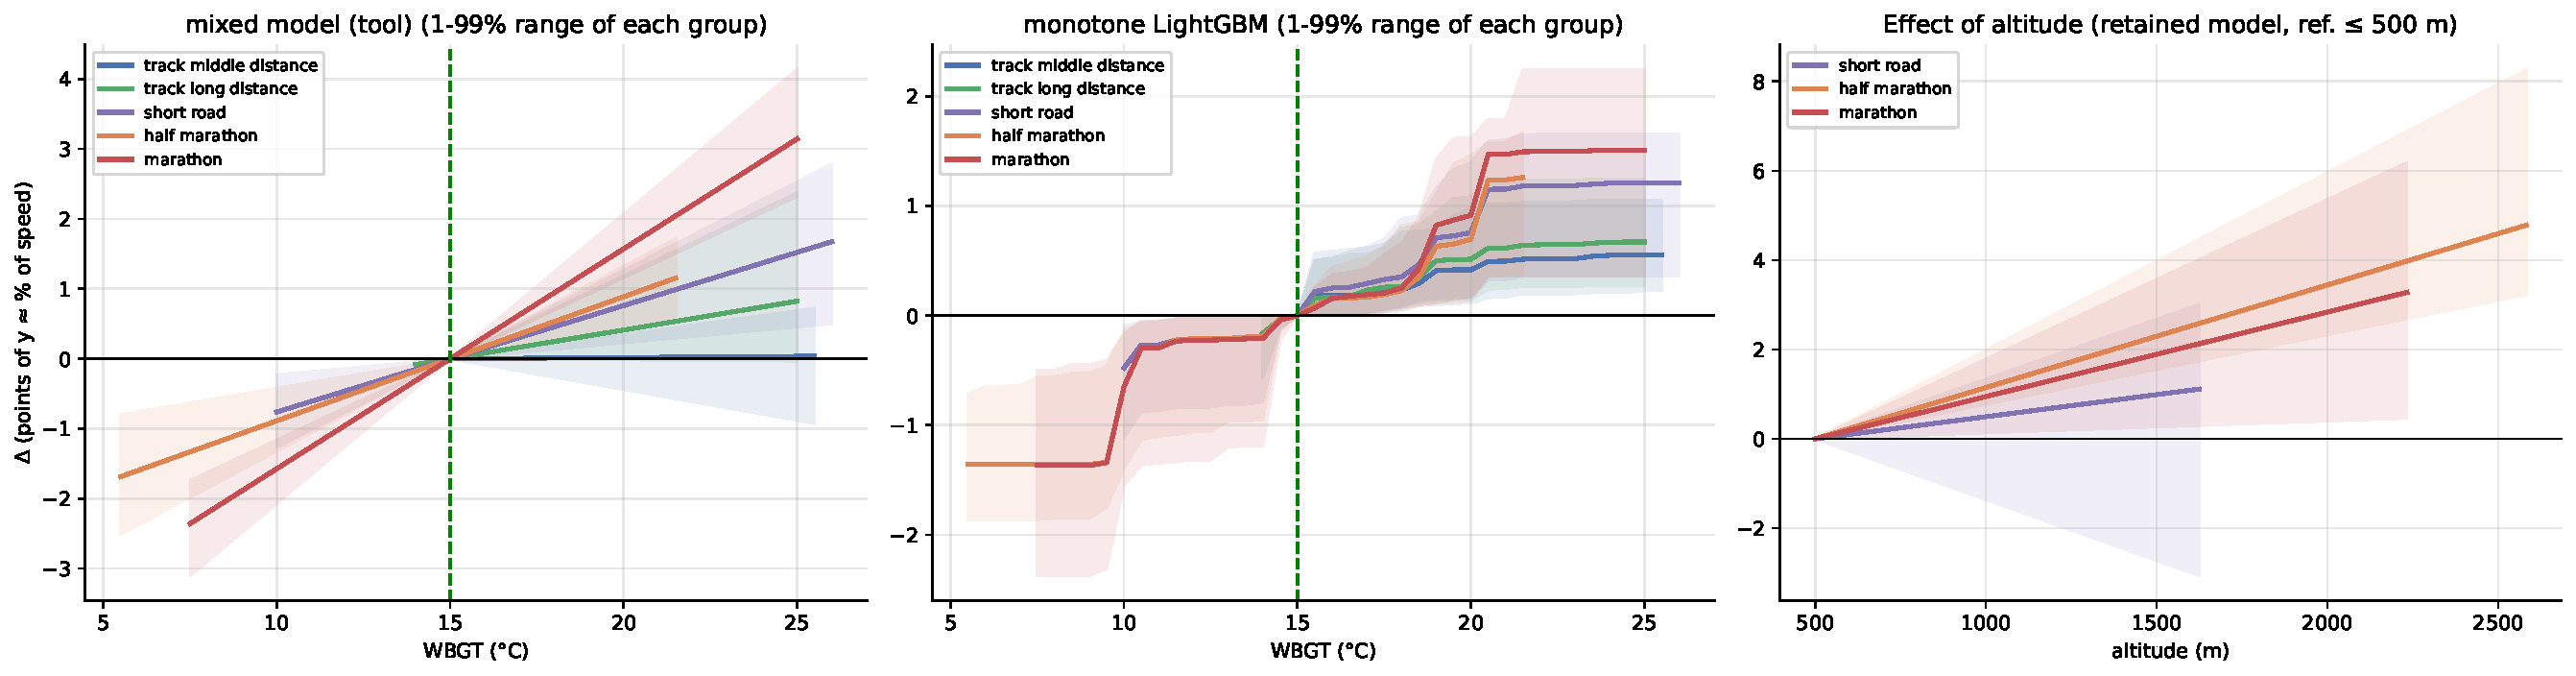
\includegraphics[width=\textwidth]{final_curves}
\caption{Degradation curves by event group, over the range from the 1st to the 99th percentile of the WBGT of each
group, with pointwise 95\% confidence bands from a venue bootstrap: tool's model (left, 300 replicates) and monotone
boosting (center, 50 replicates). Right, effect of altitude estimated by the tool's model, relative to an altitude
below 500~m.}
\label{fig:final_curves}
\end{figure}

The effect grows with the duration of the effort, as physiology predicts: stored heat accumulates and cardiovascular
drift sets in as the effort goes on. It is zero in middle distance, where an 800~m or a 1,500~m is too short for
thermoregulation to limit performance; the interval, centered on 0, rules out an effect larger than 0.7~point at
25~°C. It is about 0.8~point in track long distance, with an interval that touches 0, then about 1.5~points in short
road races. It reaches about 3~points in the marathon between 15 and 25~°C, that is, about 4~min~45~s for a 2:30
marathon, the order of magnitude reported by \citet{ely2007}. The half marathon at 25~°C is an extrapolation, since no
race was observed above 22~°C. The effects being linear, the effect at 25~°C is twice that at 20~°C; yet the class means
suggested an acceleration beyond 20~°C in the marathon, so that the model may slightly underestimate the effect around
25~°C and overestimate it around 18 to 20~°C. Weighted by the group sizes, the effect of a 10~°C increase is about
1.7~points, slightly less than the estimates of section~\ref{sec:which_estimator} (1.9 to 2.4~points), obtained on the
training venues only with an effect common to all events, but of the same order of magnitude.

The other terms complete the picture. Wind costs $0.36$~point for 2~m/s more at 10~m (interval $[0.08, 0.63]$), at equal
WBGT: its cooling effect already goes through the WBGT, and what remains is the mechanical effect, a headwind not being
compensated by a tailwind. Rain, too rare, does not allow a conclusion ($+0.34$ for 1~mm/h, interval
$[-0.53, 2.00]$). The difference between slow and fast runners predicted by \citet{ely2007} is not detected in the
marathon: for a 10~°C increase, a runner of level $+10$ loses $0.17$~point less than a runner of level $-10$, with an
interval $[-1.24, 0.86]$; our data contain only good runners, over a narrow range of levels. Altitude, finally, costs
about 1.9~points in the marathon at 1,500~m (interval $[0.05, 3.65]$) and 2.3~points in the half marathon
($[1.55, 4.48]$), and remains undetermined in short road races ($+0.99$, interval $[-2.95, 2.80]$). These effects rest
on 3 to 6 venues per group, hence the width of the intervals, and may also reflect the specific courses of these
cities.

The monotone boosting, kept as a point of comparison, gives the same ranking of events and close values up to 20~°C,
but it levels off beyond: about $+1.5$~points in the marathon at 25~°C, against 3.1 for the mixed model. The
monotonicity constraint has another effect, visible in middle distance: its curve cannot fall below 0 above 15~°C, and
rises to about $+0.5$~point with an interval that excludes 0, whereas the mixed model finds a zero effect. This is the
announced bias: when the true effect is zero, a curve constrained to rise can only overestimate it. The two models agree,
on the other hand, on the cool side: in the marathon, running at 7 or 8~°C rather than at 15~°C saves 1.4 to
2.4~points.

\section{Prediction uncertainty}\label{sec:uncertainty}

Two kinds of uncertainty must not be confused. The \emph{confidence interval} concerns a parameter or a mean effect,
here the degradation curve $\Delta(W)$: it reflects the imprecision due to the finite sample size, and would shrink to
zero with more venues and races. The \emph{prediction interval}
$\hat I(x) = [\hat q_{\text{low}}(x), \hat q_{\text{high}}(x)]$ concerns a future observation: it must contain an
athlete's performance $y$ with probability $1 - \alpha$. Even with a perfect model, known without error, it remains as
wide as the individual noise, and does not shrink with more data. An honest tool must be able to state both; we sought
to build 90\% prediction intervals ($\alpha = 0.1$).

\subsection{Quantile regression and the pinball loss}\label{sec:pinball}

The mean minimizes the squared loss and the median the absolute loss. More generally, the quantile of order $\alpha$ of
a variable $Y$, the value $q$ such that $\mathbb{P}(Y \leq q) = \alpha$, minimizes the expectation of the
\emph{pinball loss}
\[
\rho_\alpha(y, q) = \max\big(\alpha\,(y - q),\ (\alpha - 1)(y - q)\big) =
\begin{cases} \alpha\,(y - q) & \text{if } y \geq q, \\ (1 - \alpha)\,(q - y) & \text{if } y < q. \end{cases}
\]
Indeed, for a variable $Y$ with continuous cumulative distribution function $F$,
\[
\E[\rho_\alpha(Y, q)] = \alpha\int_{q}^{+\infty}(y - q)\,\dd F(y) + (1 - \alpha)\int_{-\infty}^{q}(q - y)\,\dd F(y),
\]
whose derivative with respect to $q$ is $-\alpha\,\big(1 - F(q)\big) + (1 - \alpha)\,F(q) = F(q) - \alpha$. It vanishes
when $F(q) = \alpha$, and the function is convex: the minimum is reached at the quantile of order $\alpha$. A
prediction that is too low costs $\alpha$ per unit and one that is too high $1 - \alpha$: for $\alpha = 0.95$, being too
low costs 19 times more than being too high, and $q$ is placed high enough for 95\% of the observations to fall below
it. For $\alpha = 0.5$, we recover the absolute loss and the median.

By minimizing the mean pinball loss on the data instead of the squared error, a model estimates a conditional quantile
$\hat q_\alpha(x)$: this is \emph{quantile regression} \citep{koenker1978}. Two boostings, for the orders $0.05$ and
$0.95$, give a ``raw'' 90\% prediction interval, whose width adapts to $x$. Nothing, however, guarantees its coverage:
learned on the training data, these quantiles ignore the estimation error of the model itself and the difference
between the training venues and a new venue.

\subsection{Conformal prediction}\label{sec:conformal}

\emph{Conformal prediction} \citep{vovk2005} corrects this flaw by calibrating the interval on a separate set of $n$
observations, not used for training. A \emph{nonconformity score} $s_i$ is computed on this set, all the larger as
observation $i$ is poorly predicted, then the threshold $\hat q$, equal to the $\lceil (n+1)(1-\alpha)\rceil$-th
smallest value of the scores (and $+\infty$ if this index exceeds $n$). The prediction interval retained is the set of
values $y$ whose score would be less than or equal to $\hat q$.

The guarantee rests on a single assumption: the scores of the $n$ calibration observations and that of a new
observation are \emph{exchangeable}, that is, their joint distribution is unchanged when they are permuted. This is the
case if they are independent and identically distributed, but the assumption is weaker. Under this assumption, and in
the absence of ties, the rank of the new score among the $n + 1$ scores is uniform on $\{1, \dots, n + 1\}$: the new
score is therefore less than or equal to the $k$-th smallest calibration value with probability at least $k/(n + 1)$.
With $k = \lceil (n+1)(1-\alpha)\rceil$, we obtain
\begin{equation}\label{eq:conformal_guarantee}
\mathbb{P}\big(y \in \hat I(x)\big) \geq \frac{\lceil (n+1)(1-\alpha)\rceil}{n + 1} \geq 1 - \alpha .
\end{equation}
The guarantee holds in finite samples, whatever the quality of the model and without any assumption on the
distribution of the data: a poor model gives wide intervals, but always well calibrated ones. The $n + 1$ correction
matters, the ordinary empirical quantile slightly undercovering, especially for a small calibration set.

We compared two scores. The simple conformal score, $s_i = |y_i - \hat y(x_i)|$, is the absolute error of a model of the
mean; the interval $\hat y(x) \pm \hat q$ has constant width, as wide for an 800~m as for a marathon. Conformalized
quantile regression \citep[CQR,][]{romano2019} starts instead from the raw quantiles, with the score
$s_i = \max\big(\hat q_{\text{low}}(x_i) - y_i,\ y_i - \hat q_{\text{high}}(x_i)\big)$, which measures by how much $y_i$
exceeds the raw interval and is negative if $y_i$ lies inside it. The interval
$[\hat q_{\text{low}}(x) - \hat q, \hat q_{\text{high}}(x) + \hat q]$ keeps the adaptive width of the raw quantiles,
widened, or narrowed if $\hat q < 0$, just enough to reach the desired coverage. In both cases, the guarantee is
\emph{marginal}: it concerns the proportion of performances covered on average, and does not guarantee coverage
\emph{conditional} on a subgroup, such as marathons. Some groups can be over-covered and others under-covered, the
average remaining correct.

We trained three boostings, the mean with the monotonicity constraint and the quantiles of orders $0.05$ and $0.95$,
on four folds of venues, calibrated on the fifth fold, and evaluated on the test venues. Calibrating on venues the
model had not seen was meant to reproduce the situation of a new venue. Exchangeability is, however, only approximate:
calibration and test concern different venues, and performances of the same race are correlated.

\subsection{A guarantee that fails, and why}\label{sec:undercoverage}

On the test venues, the raw quantiles cover 86.8\% of performances, for a mean width of 8.13~points. The simple
conformal interval ($\hat q = 3.655$) covers 83.4\% for a width of 7.31, and CQR ($\hat q = -0.211$) 84.2\% for a width
of 7.71. The pinball losses on the test set are 0.242 for the quantile of order 0.05 and 0.355 for that of order 0.95.
The calibrated intervals therefore undercover: they cover only 83 to 84\% of performances instead of the guaranteed
90\%, and even do worse than the raw quantiles.

Guarantee \eqref{eq:conformal_guarantee} is not wrong: it is its assumption that is not satisfied. The calibration fold
is fold~0, the easiest of the five: the constant model obtained an RMSE of 2.65 there, against 3.19 on the test venues.
Its performances, less dispersed, give smaller scores than those of the test venues: calibration and test scores are
not exchangeable, the threshold $\hat q$ is too small and the interval too narrow. The sign of the CQR threshold shows
it clearly: $\hat q$ is negative, which means that, on the calibration fold, the raw quantiles seemed too wide, and CQR
narrowed them even though they were already slightly too narrow for the test venues. A conformal guarantee holds only
if the calibration set is representative of the data to which it is applied. With data grouped by venue, very
heterogeneous from one venue to another, a fold of 14 venues is not enough to represent between-venue variability. Two
remedies are possible: calibrating on several folds, using the out-of-fold predictions of cross-validation, or
calibrating by event group.

CQR adapts the width to the event well: 5.0~points in middle distance, 6.3 in track long distance, 8.4 in short road
races, 9.7 in the half marathon and 10.4 in the marathon, which reflects the heteroscedasticity observed from the
exploration stage onward. Its coverage nevertheless varies from 79.6\% in middle distance to 88.6\% in the half
marathon, with 86.8\% in track long distance, 85.1\% in short road races and 85.8\% in the marathon: the guarantee,
already approximate on average, does not hold group by group.

These prediction intervals, of about $\pm 4$~points, are much wider than the confidence interval of the degradation
curve, from $\pm 0.4$ to $\pm 1$~point. The former concerns the time of an individual performance and includes form on
the day, tactics and the age of the personal best, a noise with a standard deviation close to 2.8~points that does not
decrease with sample size; the latter concerns the mean effect of the conditions, which becomes more precise with more
data. To set a pace, it is $\Delta$ and its confidence interval that matter: the question is ``by how much should I
slow down to produce the same effort'', not ``what time will I run''. The upper bound of the confidence interval gives
a cautious pace. The prediction interval, for its part, is a reminder that an individual race time remains very
uncertain, whatever the conditions.

\section{The tool: equal-effort speed}\label{sec:tool}

\subsection{From the model to the equivalent speed}\label{sec:conversion_steps}

The tool takes as input the target speed $Y$ in reference conditions, the conditions of the day $\mathcal{C}$
(temperature, humidity, wind at 10~m, global radiation, rain, altitude, as well as the date, time and place, which set
the position of the sun), the event and the sex. The reference conditions $\mathcal{C}_{\text{ref}}$ are a WBGT of
15~°C, a wind of 2~m/s at 10~m, no rain and an altitude of at most 500~m. The computation follows five steps.

The WBGT of the day is first computed with the Liljegren model. Pressure is derived from the altitude $z$, in meters,
with the barometric formula of the standard atmosphere,
\[
p(z) = 1013.25\,\big(1 - 2.2557\cdot 10^{-5}\,z\big)^{5.2559}\ \text{hPa},
\]
which follows from the hydrostatic equilibrium of an atmosphere whose temperature decreases linearly with altitude:
$2.2557\cdot10^{-5} = L/T_0$, with a lapse rate $L = 0.0065$~K/m and a ground temperature $T_0 = 288.15$~K, and
$5.2559 = g_0 M/(R L)$, where $g_0$ is the gravitational acceleration, $M$ the molar mass of air and $R$ the gas
constant. At 1,000~m, pressure is 11\% lower than at sea level.

The athlete's implicit profile is then built. Their speed $Y$ corresponds, over the distance $d$, to a time
$t_Y = d/Y$, which is treated as their personal best: their level is $100\ln(t_Y/t^{\PB}_{\text{med}})$, where
$t^{\PB}_{\text{med}}$ is the median personal best for the sex and event, and their expected duration is $t_Y/60$
minutes.

The degradation $\Delta = f(\mathcal{C}) - f(\mathcal{C}_{\text{ref}})$ is then computed on a set of actual
performances of the same event and sex, up to 200: they are given the athlete's profile, the conditions $\mathcal{C}$
are imposed, then the reference conditions (WBGT, wind, rain \emph{and} altitude), and the difference of the
predictions is averaged. This is a mean of ICE curves, which integrates over the other variables (age, form, time of
day) observed for this type of race. The reference conditions must fix all the meteorological variables: otherwise,
$\Delta$ would mix the effect of the conditions of the day with that of the conditions observed in the reference
population.

The equivalent speed is finally $X = Y\,e^{-\Delta/100}$, from \eqref{eq:conversion}. Its confidence interval comes from
the 300 bootstrap models: with $\Delta_{0.025}$ and $\Delta_{0.975}$ the quantiles of the bootstrap degradations,
$X_{\text{low}} = Y\,e^{-\Delta_{0.975}/100}$ and $X_{\text{high}} = Y\,e^{-\Delta_{0.025}/100}$. The function
$\Delta \mapsto Y e^{-\Delta/100}$ being decreasing, the lower bound of the speed corresponds to the upper bound of the
degradation, and the quantiles carry over without approximation. The first-order approximation
$X \approx Y(1 - \Delta/100)$ would be all the worse as $\Delta$ is large, $\Delta$ being expressed in logarithmic
percent.

The last step is a safeguard: if the WBGT of the day falls outside the range observed for the event group (between its
1st and 99th percentiles), or if the altitude exceeds that observed for this group, the tool does not answer. These
ranges go from 16.0 to 25.6~°C in middle distance, from 13.5 to 25.2~°C in track long distance, from 9.8 to 27.4~°C in
short road races, from 5.2 to 21.8~°C in the half marathon and from 7.3 to 25.1~°C in the marathon. A linear model
would obediently extend its line beyond the data; we preferred a tool that does not answer to a tool that answers
wrongly.

\subsection{Inversion: from the speed run to the reference speed}\label{sec:inversion}

The inverse problem is the following: ``I ran at speed $X$ in conditions $\mathcal{C}$; what speed is it worth in
reference conditions?'' One must find the root $Y$ of
\[
r(Y) = Y\,e^{-\Delta(\mathcal{C};\,Y)/100} - X .
\]
Since $\Delta$ depends on $Y$, through the athlete's level and expected duration, there is no closed form, and we solve
numerically with Brent's method \citep{brent1973}. The root is first bracketed, $r(0.8\,X) < 0 < r(1.25\,X)$, since the
degradation remains of a few percent. Bisection then guarantees convergence: the interval is cut in two and the half
where $r$ changes sign is kept, so that the width is halved at each iteration and a precision of $10^{-7}$ is reached in
about thirty iterations. Brent's method combines this safety with two faster methods, the secant method, which
replaces $r$ by the line through two points, and inverse quadratic interpolation, which uses a parabola through three
points. It uses the fast method when it makes progress, and falls back on bisection otherwise: convergence is
guaranteed as soon as $r(a)\,r(b) < 0$, and fast when $r$ is smooth.

\subsection{A few examples}\label{sec:examples}

The WBGT computation was first checked in two situations: 20~°C and 50\% humidity in the shade give a WBGT of 15.2~°C,
close to the reference, and 30~°C, 70\% humidity and a sun of 600~W/m² give 31.0~°C, beyond the ACSM black flag. A
marathon runner running at $Y = 4.80$~m/s in reference conditions (2:26:30), at 22~°C and 60\% humidity in the shade
(WBGT of 18.1~°C), loses $\Delta = +0.93$~point: the tool advises $X = 4.7554$~m/s, with a confidence interval from
4.7365 to 4.7734~m/s, and the inversion recovers the starting speed exactly, $Y = 4.80000$~m/s.

Take a 2:30 marathon runner in reference conditions. In cool weather, 15~°C in the shade and 70\% humidity (WBGT of
12.4~°C, below the reference), the tool advises them to run faster: 2:28:49 (interval from 2:28:17 to 2:29:20). At
22~°C, 70\% humidity and a sun of 300~W/m² (WBGT of 21.9~°C), their reference marathon is worth 2:33:10, with an
interval from 2:31:47 to 2:34:38. The effect is almost identical for a 2:50 female marathon runner in the same
conditions ($+2.12$\%, that is, 2:53:38): the model does not distinguish the sexes in the effect of heat. At 27~°C and
80\% in the sun, the WBGT (27.5~°C) exceeds the 99th percentile observed in the marathon, and the tool refuses to
answer. At an altitude of 1,500~m and 15~°C, the marathon loses about 1\% (2:31:35), but the interval, from 2:28:44 to
2:34:35, contains the reference: the effect of altitude remains very uncertain. Over 10~km, a female runner of 35:00 in
reference conditions is worth 35:31 at 25~°C, 75\% humidity and 300~W/m² (WBGT of 25.2~°C). On the track, finally,
even at 28~°C (WBGT of 22.4~°C), the pace does not change: a 3:50 1,500~m remains at 3:50, with an interval that does
not exceed one or two seconds on either side.

\subsection{A temperature--humidity chart}\label{sec:chart}

A runner reasons in terms of temperature and humidity, not WBGT. The chart translates the tool into these terms: for
an event, a sex, a reference speed, a wind and a radiation, the WBGT is computed on a grid of temperatures (5 to 40~°C)
and humidities (10 to 100\%), then the degradation $\Delta$ in each cell. With wind, rain and altitude fixed, the model
depends on the weather only through the WBGT: it is therefore enough to evaluate $\Delta$ and its bootstrap quantiles on
a grid of WBGT values covering the range of the group, then to interpolate for each cell. Each situation is represented
by two panels: the central estimate of $\Delta$, and the upper bound of its 95\% confidence interval, that is, the
strongest slowdown compatible with the data, the cautious bound for setting a pace (figure~\ref{fig:chart}).

\begin{figure}[htbp]
\centering
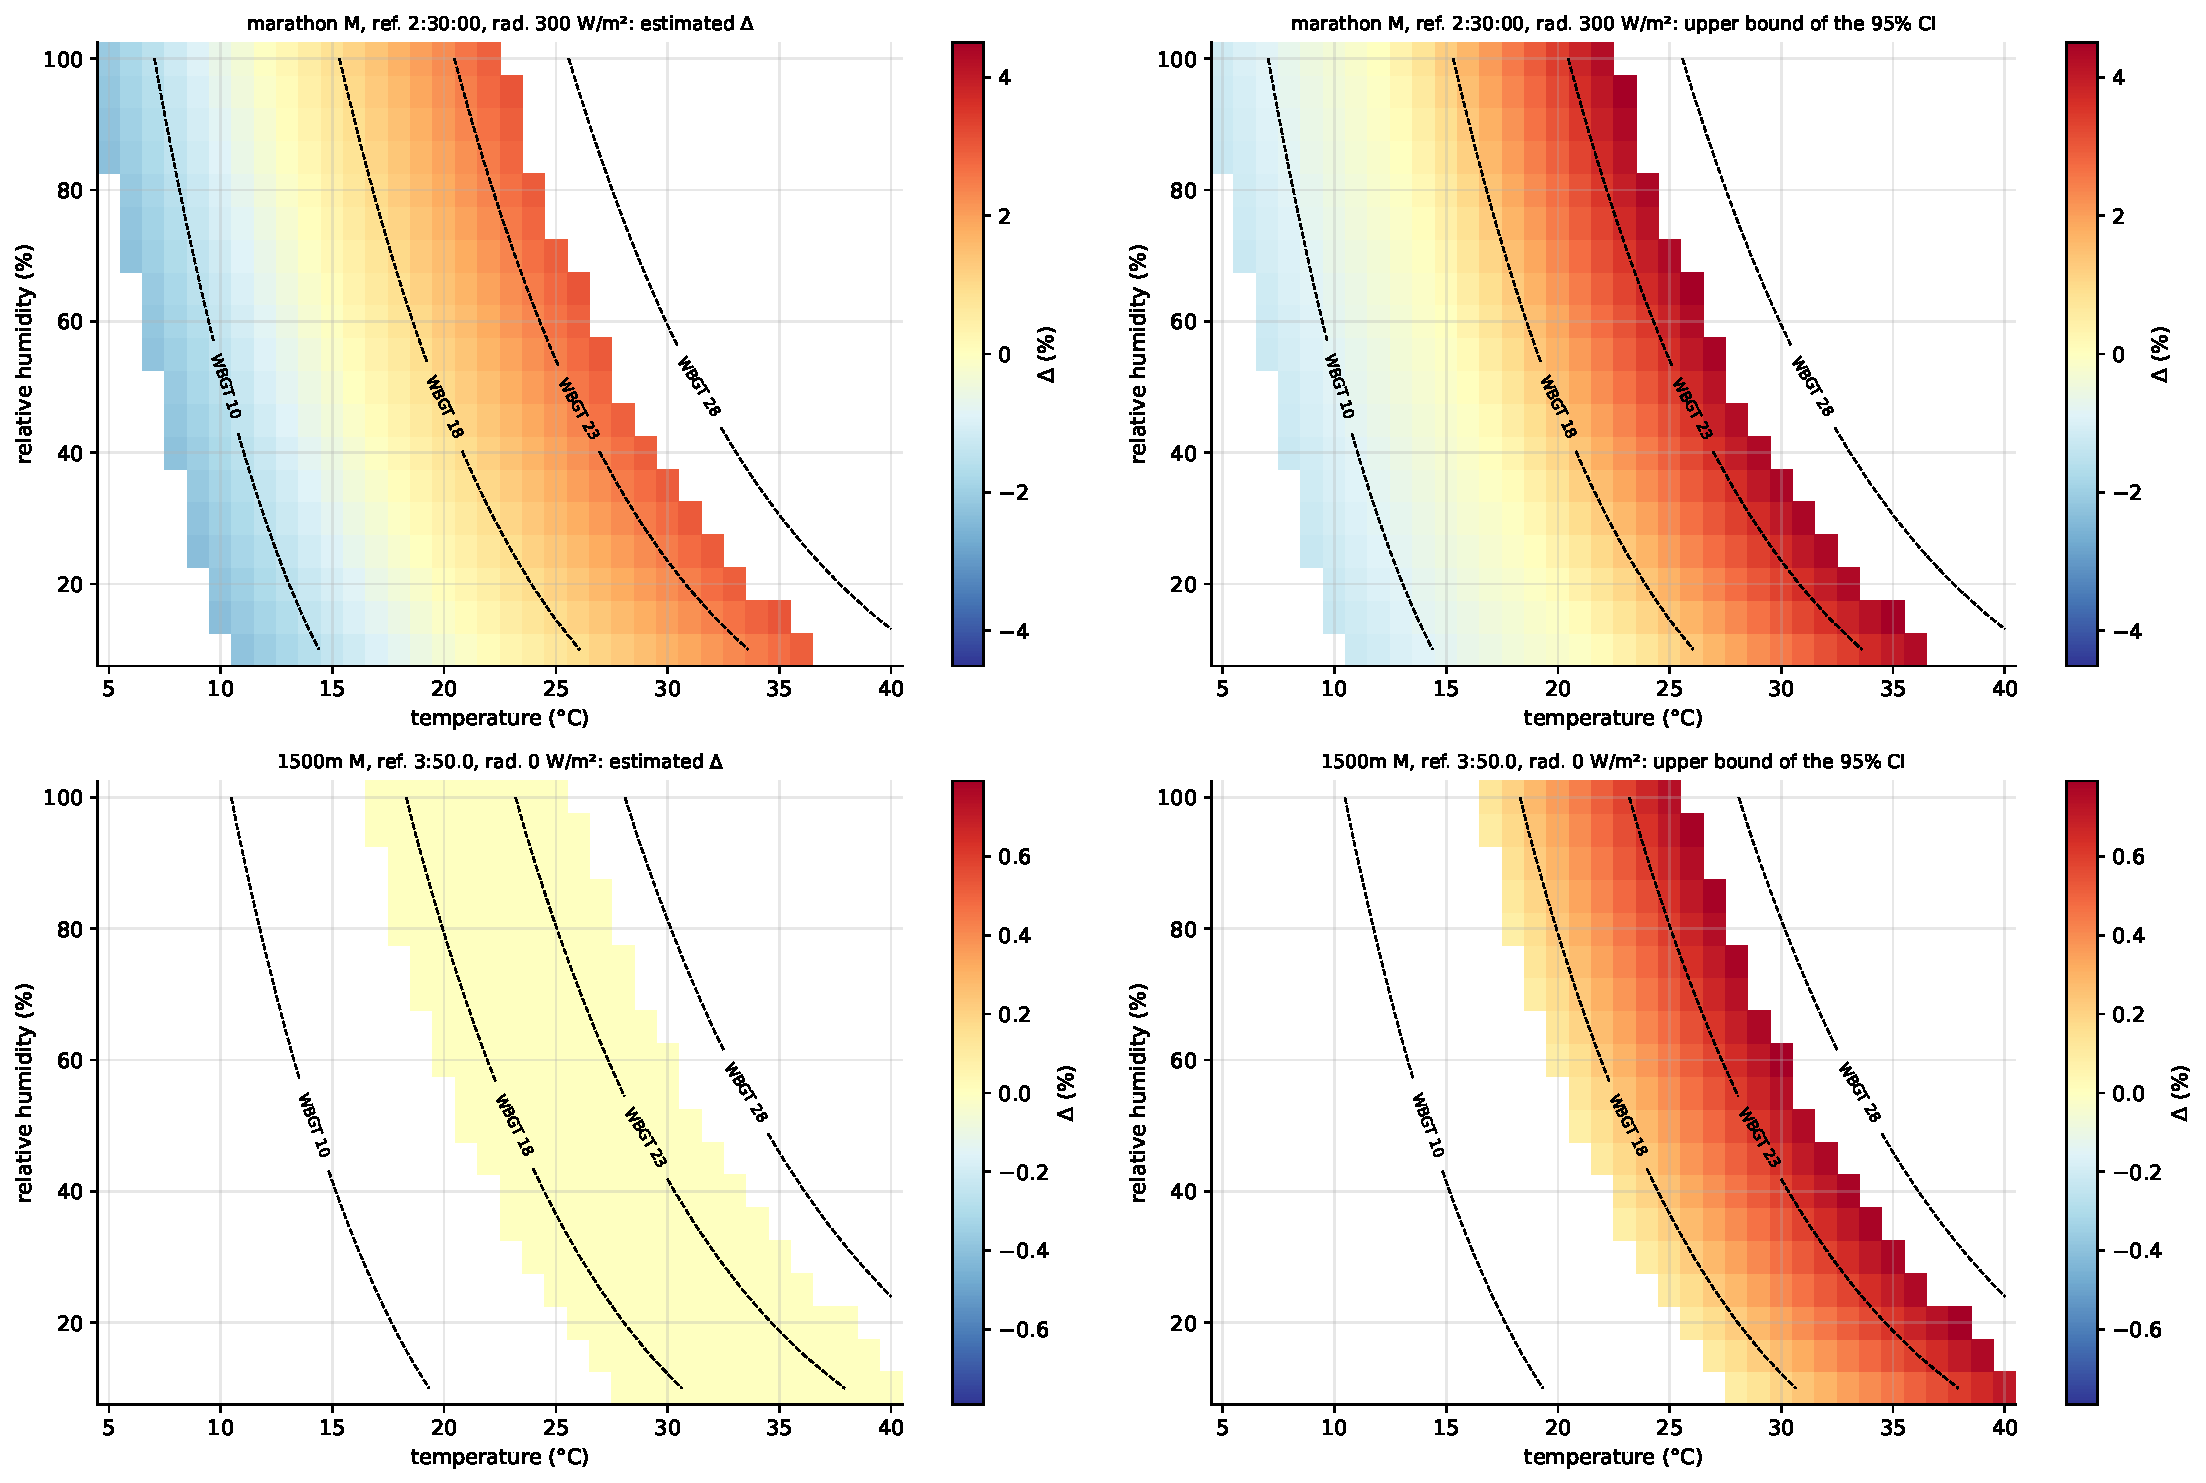
\includegraphics[width=\textwidth]{chart}
\caption{Chart of the degradation $\Delta$ as a function of temperature and relative humidity, for a men's 2:30
marathon in reference conditions, with a sun of 300~W/m² (top), and a men's 3:50 1,500~m, run in the evening without
sun (bottom). Left, central estimate; right, upper bound of the 95\% confidence interval. The WBGT isolines 10, 18, 23
and 28~°C correspond to the ACSM thresholds; white cells fall outside the range observed for the event group.}
\label{fig:chart}
\end{figure}

In the marathon, the WBGT isolines go down from left to right: at equal temperature, humidity increases the heat load,
and the sun alone adds several degrees of WBGT compared with the shade. The degradation ranges from $-2.3$\% for a WBGT
of 8 to 10~°C, where one runs faster than in reference conditions, to $+3.0$\% around 25~°C; the cautious bound ranges
from $-1.3$ to $+4.5$\%. At 22~°C, 70\% humidity and in the sun, the tool advises 2:33:10, that is, about 3:38 per
kilometer instead of 3:33. Table~\ref{tab:chart} gives the equivalent times for a few combinations. Overall, 41\% of the
cells are white, in humid heat as well as in dry cold: the tool refuses to answer rather than extrapolate a straight
line. Over 1,500~m, the degradation is zero (less than 0.01~point in absolute value) over the whole covered range, from
16 to 25.6~°C, and the upper bound stays below 0.8\%, less than two seconds over 3:50. But 70\% of the grid is white:
our data contain no cool track meeting, and the tool says nothing about a 1,500~m in cool weather.

\begin{table}[htbp]
\centering
\small
\caption{Times equivalent to a men's 2:30 marathon in reference conditions, by temperature and relative humidity, with
a sun of 300~W/m² and a wind of 2~m/s: central estimate, then cautious time (bound of the 95\% confidence interval). A
dash marks a combination outside the observed range.}
\label{tab:chart}
\begin{tabular}{@{}lccccc@{}}
\toprule
& 10~°C & 15~°C & 20~°C & 25~°C & 30~°C \\
\midrule
RH 30\% & 2:27:03 / 2:28:20 & 2:28:48 / 2:29:20 & 2:30:34 / 2:30:51 & 2:32:21 / 2:33:30 & 2:34:09 / 2:36:11 \\
RH 50\% & 2:27:40 / 2:28:41 & 2:29:34 / 2:29:45 & 2:31:30 / 2:32:14 & 2:33:27 / 2:35:09 & -- \\
RH 70\% & 2:28:14 / 2:29:00 & 2:30:16 / 2:30:24 & 2:32:20 / 2:33:28 & 2:34:27 / 2:36:38 & -- \\
RH 90\% & 2:28:46 / 2:29:18 & 2:30:55 / 2:31:21 & 2:33:06 / 2:34:37 & -- & -- \\
\bottomrule
\end{tabular}
\end{table}

The pacing advice that follows is simple. Over 1,500~m, no adjustment is justified. In the marathon, one should slow
down by 1 to 1.5\% per 5~°C of WBGT above 15~°C, and aim for the cautious bound if one does not know one's heat
tolerance. These figures are averages for good runners, acclimatized or not, without distinction; individual
tolerance, acclimatization and hydration can weigh much more. Beyond 23~°C of WBGT, the threshold of the ACSM red flag,
the issue becomes safety rather than the race time.

\section{Discussion}\label{sec:discussion}

\subsection{Truncation, revisited with the final model}\label{sec:sensitivity}

Exploration had shown that the truncation of the lists attenuates the raw slope of heat, and we had retained a minimum
margin of 5\% as a compromise. It remained to check that our conclusions do not depend on it. We re-estimated the
tool's model for several minimum margins $M$, on the valid performances with a margin of at least $M$, and computed in
each event group the effect of a WBGT increase from 15 to 25~°C (table~\ref{tab:margins}). If truncation attenuates the
effect of heat, this effect must increase with $M$.

\begin{table}[htbp]
\centering
\small
\caption{Effect of a WBGT increase from 15 to 25~°C, in points of $y$, estimated by the tool's model according to the
minimum truncation margin $M$ required.}
\label{tab:margins}
\begin{tabular}{@{}rrccccc@{}}
\toprule
$M$ & Performances & Track middle dist. & Track long dist. & Short road & Half marathon & Marathon \\
\midrule
0\% & 14,221 & $-0.06$ & 0.50 & 1.08 & 1.74 & 3.36 \\
3\% & 12,275 & 0.01 & 0.53 & 1.30 & 1.71 & 3.23 \\
5\% & 10,398 & 0.04 & 0.82 & 1.52 & 1.78 & 3.14 \\
8\% & 7,637 & $-0.02$ & 0.79 & 1.62 & 1.88 & 3.16 \\
12\% & 4,514 & $-0.34$ & 1.86 & 1.72 & 1.44 & 3.02 \\
\bottomrule
\end{tabular}
\end{table}

The effect of truncation is bounded. In the marathon, the effect stays between 3.0 and 3.4~points when $M$ varies from
0 to 12\%: the main result is robust to the choice of the margin. In short road races, it goes from 1.1 to 1.7~points as
$M$ increases, in the direction of an attenuation by truncation. Middle distance stays close to 0 whatever $M$. The
values at $M = 12$\% rest on samples reduced by half, and track long distance becomes unstable there. In the marathon,
the effect even decreases slightly as $M$ increases, unlike the raw slope: once the controls are introduced, truncation
no longer biases the effect in a detectable way there, and these differences remain within the uncertainty of the
estimates.

\subsection{Validity of the target}\label{sec:target_validity}

The target $y = 100\ln(t/t^{\PB})$ assumes a maximal effort and a personal best representative of the level on the day.
The personal best may be old: $y$ increases strongly with age, and age, form and level only correct for this on
average. Our data do not follow athletes, so the comparison is made between similar runners, not within the same
runner; a within-athlete design, observing the same runner in different conditions, would be more convincing. Finally,
the 6,222 performances without a published personal best, beginners over the distance or missing data, were excluded:
the sample overrepresents experienced runners.

\subsection{Possible biases and their direction}\label{sec:biases}

Several biases remain, and most of them pull the estimated effect toward zero. Measurement error in the weather is the
first of them. Our weather comes from a reanalysis with a resolution of 9 to 30~km, without microclimate (urban heat
island, stands); on the track, the time is that of the start of the meeting and not of the race. If one observes
$W^{\text{obs}} = W + \epsilon_W$ instead of the true WBGT $W$, with an error $\epsilon_W$ independent of $W$ and $y$,
then $\Cov(W^{\text{obs}}, y) = \beta_W \Var(W)$ and $\Var(W^{\text{obs}}) = \Var(W) + \Var(\epsilon_W)$, so that the
estimated slope tends to
\[
\beta_W\,\frac{\Var(W)}{\Var(W) + \Var(\epsilon_W)} < \beta_W .
\]
This is \emph{attenuation bias}: random measurement error always pulls the effect toward zero, all the more so as the
useful variation of the WBGT is small, which is the case for within-course variation. Selection also underestimates the
effect: in strong heat, dropouts are not listed, and some runners give up or manage their race. The effect is then
underestimated for the maximal race time, but this is partly what a runner wants to know: by how much to slow down in
order to finish.

Confounding between venues remains possible. Heat is mostly observed between venues, with a within-course standard
deviation of only about 1~°C, and country, field and course profile are only imperfectly controlled, even though fixed
effects and the Mundlak term agree with random effects. Heteroscedasticity, next, is only worked around: the
within-race standard deviation of $y$ doubles between the track and the marathon, and the mixed model with a common
$\sigma^2$ has a bimodal likelihood, worked around by fixing $\gamma$ but not corrected. Prediction intervals, finally,
depend on exchangeability, and an unrepresentative calibration fold makes them lose the guaranteed coverage.

\subsection{Generalization and avenues for improvement}\label{sec:generalization}

Our data cover good-level runners, a WBGT of 5 to 28~°C, the track only between 13.5 and 26~°C in the evening, and
altitude only on the road. Nothing allows extrapolation to recreational runners, more affected according to
\citet{ely2007}, to heatwaves, to championships in tropical climates or to middle distance in cold weather. For training
at submaximal pace, ``same effort'' refers rather to heart rate or perceived exertion, and the tool does not transfer
directly to it.

Several avenues would allow us to go further. Complete result lists, dropouts included, would remove truncation, and
athlete identifiers would allow a within-athlete design. Actual start times, nearby weather stations and course
profiles would reduce measurement error and confounding between venues. On the statistical side, a heteroscedastic
mixed model, with a $\sigma^2$ specific to each event group, would address the bimodality at its source; crossed random
effects athlete $\times$ race, or a hierarchical Bayesian model that would shrink the effect of heat of one event group
toward that of the others, would make it possible to estimate a common curvature. Conformal calibration on several
folds, or by event group, would restore the coverage of prediction intervals. A joint model of dropout and performance
would handle selection, and heart rate data would make it possible to transfer the tool to training.

\section{Conclusion}\label{sec:conclusion}

At equal effort, when the WBGT goes from 15 to 25~°C, heat costs nothing measurable over 800~m and 1,500~m, about 1.5\%
over 5 and 10~km and about 3\% in the marathon. Wind costs about 0.2\% per m/s at equal WBGT, and altitude weighs on
road races, with large uncertainty. In prediction, the four model families are on a par, and about one sixth of the
variance of performances is predictable on a new venue; the rest is a matter of form on the day.

The path that led there is perhaps as interesting as the result. Each difficulty encountered called for a specific
tool: the truncation of the lists, the truncated normal distribution and a minimum margin; confounding, controls,
interactions and the Mundlak decomposition; the dependence between runners of the same race, cross-validation by
venue, generalized least squares and the venue bootstrap; the disagreement between models of equal accuracy, an
interpretable model chosen on physiological criteria; the bimodality of the likelihood, a working covariance; the
undercoverage of conformal intervals, an examination of the exchangeability assumption. Four methodological lessons
emerge: validate by groups when the data are structured; estimate uncertainty with a bootstrap of the same groups;
distinguish predicting from estimating an effect; and prefer a tool that gives an honest interval and refuses to
extrapolate.

\begin{thebibliography}{99}

\bibitem[Aitken(1935)]{aitken1935}
Aitken A. C. (1935). On least squares and linear combination of observations. \emph{Proceedings of the Royal Society
of Edinburgh} 55, 42--48.

\bibitem[Armstrong et~al.(2007)]{armstrong2007}
Armstrong L. E. et~al. (2007). American College of Sports Medicine position stand. Exertional heat illness during
training and competition. \emph{Medicine \& Science in Sports \& Exercise} 39(3), 556--572.

\bibitem[Bergstra and Bengio(2012)]{bergstra2012}
Bergstra J., Bengio Y. (2012). Random search for hyper-parameter optimization. \emph{Journal of Machine Learning
Research} 13, 281--305.

\bibitem[Breiman et~al.(1984)]{breiman1984}
Breiman L., Friedman J., Olshen R., Stone C. (1984). \emph{Classification and Regression Trees}. Wadsworth.

\bibitem[Brent(1973)]{brent1973}
Brent R. P. (1973). \emph{Algorithms for Minimization without Derivatives}. Prentice-Hall.

\bibitem[Chen and Guestrin(2016)]{chen2016}
Chen T., Guestrin C. (2016). XGBoost: a scalable tree boosting system. \emph{Proceedings of the 22nd ACM SIGKDD
International Conference on Knowledge Discovery and Data Mining}, 785--794.

\bibitem[Cybenko(1989)]{cybenko1989}
Cybenko G. (1989). Approximation by superpositions of a sigmoidal function. \emph{Mathematics of Control, Signals and
Systems} 2(4), 303--314.

\bibitem[Efron(1979)]{efron1979}
Efron B. (1979). Bootstrap methods: another look at the jackknife. \emph{The Annals of Statistics} 7(1), 1--26.

\bibitem[Ely et~al.(2007)]{ely2007}
Ely M. R., Cheuvront S. N., Roberts W. O., Montain S. J. (2007). Impact of weather on marathon-running performance.
\emph{Medicine \& Science in Sports \& Exercise} 39(3), 487--493.

\bibitem[Friedman(2001)]{friedman2001}
Friedman J. H. (2001). Greedy function approximation: a gradient boosting machine. \emph{The Annals of Statistics}
29(5), 1189--1232.

\bibitem[Goldstein et~al.(2015)]{goldstein2015}
Goldstein A., Kapelner A., Bleich J., Pitkin E. (2015). Peeking inside the black box: visualizing statistical learning
with plots of individual conditional expectation. \emph{Journal of Computational and Graphical Statistics} 24(1),
44--65.

\bibitem[Grinsztajn et~al.(2022)]{grinsztajn2022}
Grinsztajn L., Oyallon E., Varoquaux G. (2022). Why do tree-based models still outperform deep learning on typical
tabular data? \emph{Advances in Neural Information Processing Systems 35, Datasets and Benchmarks Track}.

\bibitem[Hastie et~al.(2009)]{hastie2009}
Hastie T., Tibshirani R., Friedman J. (2009). \emph{The Elements of Statistical Learning}, 2nd edition. Springer.

\bibitem[Hersbach et~al.(2020)]{hersbach2020}
Hersbach H. et~al. (2020). The ERA5 global reanalysis. \emph{Quarterly Journal of the Royal Meteorological Society}
146, 1999--2049.

\bibitem[Hornik(1991)]{hornik1991}
Hornik K. (1991). Approximation capabilities of multilayer feedforward networks. \emph{Neural Networks} 4(2),
251--257.

\bibitem[Ke et~al.(2017)]{ke2017}
Ke G., Meng Q., Finley T., Wang T., Chen W., Ma W., Ye Q., Liu T.-Y. (2017). LightGBM: a highly efficient gradient
boosting decision tree. \emph{Advances in Neural Information Processing Systems} 30.

\bibitem[Kingma and Ba(2015)]{kingma2015}
Kingma D. P., Ba J. (2015). Adam: a method for stochastic optimization. \emph{International Conference on Learning
Representations}.

\bibitem[Kish(1965)]{kish1965}
Kish L. (1965). \emph{Survey Sampling}. Wiley.

\bibitem[Koenker and Bassett(1978)]{koenker1978}
Koenker R., Bassett G. (1978). Regression quantiles. \emph{Econometrica} 46(1), 33--50.

\bibitem[Leshno et~al.(1993)]{leshno1993}
Leshno M., Lin V. Y., Pinkus A., Schocken S. (1993). Multilayer feedforward networks with a nonpolynomial activation
function can approximate any function. \emph{Neural Networks} 6(6), 861--867.

\bibitem[Liang and Zeger(1986)]{liang1986}
Liang K.-Y., Zeger S. L. (1986). Longitudinal data analysis using generalized linear models. \emph{Biometrika} 73(1),
13--22.

\bibitem[Liljegren et~al.(2008)]{liljegren2008}
Liljegren J. C., Carhart R. A., Lawday P., Tschopp S., Sharp R. (2008). Modeling the wet bulb globe temperature using
standard meteorological measurements. \emph{Journal of Occupational and Environmental Hygiene} 5(10), 645--655.

\bibitem[Lorenzo et~al.(2010)]{lorenzo2010}
Lorenzo S., Halliwill J. R., Sawka M. N., Minson C. T. (2010). Heat acclimation improves exercise performance.
\emph{Journal of Applied Physiology} 109(4), 1140--1147.

\bibitem[Loshchilov and Hutter(2019)]{loshchilov2019}
Loshchilov I., Hutter F. (2019). Decoupled weight decay regularization. \emph{International Conference on Learning
Representations}.

\bibitem[Lundberg and Lee(2017)]{lundberg2017}
Lundberg S. M., Lee S.-I. (2017). A unified approach to interpreting model predictions. \emph{Advances in Neural
Information Processing Systems} 30.

\bibitem[Lundberg et~al.(2020)]{lundberg2020}
Lundberg S. M., Erion G., Chen H., DeGrave A., Prutkin J. M., Nair B., Katz R., Himmelfarb J., Bansal N., Lee S.-I.
(2020). From local explanations to global understanding with explainable AI for trees. \emph{Nature Machine
Intelligence} 2(1), 56--67.

\bibitem[Mantzios et~al.(2022)]{mantzios2022}
Mantzios K. et~al. (2022). Effects of weather parameters on endurance running performance: discipline-specific
analysis of 1258 races. \emph{Medicine \& Science in Sports \& Exercise} 54(1), 153--161.

\bibitem[Mundlak(1978)]{mundlak1978}
Mundlak Y. (1978). On the pooling of time series and cross section data. \emph{Econometrica} 46(1), 69--85.

\bibitem[Patterson and Thompson(1971)]{patterson1971}
Patterson H. D., Thompson R. (1971). Recovery of inter-block information when block sizes are unequal.
\emph{Biometrika} 58(3), 545--554.

\bibitem[Racinais et~al.(2015)]{racinais2015}
Racinais S. et~al. (2015). Consensus recommendations on training and competing in the heat. \emph{British Journal of
Sports Medicine} 49(18), 1164--1173.

\bibitem[Romano et~al.(2019)]{romano2019}
Romano Y., Patterson E., Candès E. (2019). Conformalized quantile regression. \emph{Advances in Neural Information
Processing Systems} 32.

\bibitem[Rønnestad et~al.(2022)]{ronnestad2022}
Rønnestad B. R. et~al. (2022). Heat suit training increases hemoglobin mass in elite cross-country skiers.
\emph{Scandinavian Journal of Medicine \& Science in Sports} 32(7), 1089--1098.

\bibitem[Shapley(1953)]{shapley1953}
Shapley L. S. (1953). A value for n-person games. In \emph{Contributions to the Theory of Games}, vol. II, 307--317.
Princeton University Press.

\bibitem[Srivastava et~al.(2014)]{srivastava2014}
Srivastava N., Hinton G., Krizhevsky A., Sutskever I., Salakhutdinov R. (2014). Dropout: a simple way to prevent
neural networks from overfitting. \emph{Journal of Machine Learning Research} 15, 1929--1958.

\bibitem[Telgarsky(2016)]{telgarsky2016}
Telgarsky M. (2016). Benefits of depth in neural networks. \emph{Conference on Learning Theory}, 1517--1539.

\bibitem[Vovk et~al.(2005)]{vovk2005}
Vovk V., Gammerman A., Shafer G. (2005). \emph{Algorithmic Learning in a Random World}. Springer.

\bibitem[Zippenfenig(2023)]{zippenfenig2023}
Zippenfenig P. (2023). Open-Meteo.com Weather API. Zenodo, doi:10.5281/zenodo.7970649.

\end{thebibliography}

\end{document}
